\documentclass[12pt, a4paper]{article}

\usepackage{physics} 
\usepackage{siunitx}
\usepackage{enumerate} 
\usepackage{pgfplots}
\usepackage{booktabs}
\usepackage{hyperref}
\usepackage{tabulary}
\usepackage{amsmath}%I added this so that you can use the align tool for equations!
\usepackage{amssymb}
\usepackage{microtype}%to improve typography in the document
\pgfplotsset{compat=1.14}
\usepackage{geometry}
 \geometry{
 a4paper,
 total={170mm,257mm},
 left=20mm,
 top=20mm,
 }

\begin{document}

\title{Cosmologia}
\author{Luca Pezzini \\ Laurea Magistrale in Astrofisica \\ Universit\`{a} degli Studi di Torino, Italy}
\date{\today}

\maketitle
\newpage
\tableofcontents
\newpage
\section{Universo omogeneo ed isotropo}
L'equazione di Einstein contiene al suo interno 10 eq. diff. non lin. al second'ordine funzione del tensore metrico; data la complessità ci si mette in condizione di semplificare il sistema.\\ 
\textbf{Principio Cosmologico}: L'universo a larga scala (100 Mpc) è omogeneo ed isotropo, quindi abbiamo invarianza per traslazioni e  rotazioni spaziali (confermato da CMB), ma non per traslazioni temporali senn\'{o} avremmo il principio cosmologico perfetto con \textbf{universo  statico}.
\subsection{Risolvo equazioni di Einstein}
Risolviamo l'equazione di Einstein sotto queste prop., ricavo dunque il tensore metrico.
\begin{itemize}
    \item \textbf{Metrica O-I 4D}: superfice sferica immersa in ${\rm I\!R^3}$.
    \item \textbf{Coordinate Coomoventi}: la coord. spaziale varia in funzione del tempo risp. ad un arbitrario SR \textbf{uniformemente}, dunque una volta  nota la variazione temporale del \textbf{fattore di scala} $a(t)$ e la posizione della griglia a $t_0$ la conosco ad ogni $t$.
    \item \textbf{Metrica di F-R-W}: metrica di un fluido O-I in espansione uniforme. Funzione della curvatura dello spazio tempo $k(t)= R(t)^{-1}$, che espandendosi varia mantenendo costante il segno.
\end{itemize}
\begin{equation}
    ds^2 = c^2 dt^2 - a(t)[dr^2 - k^{-1} S_k^2(\tau \sqrt{\abs{k}})(d\theta^2 + sin^2\theta d\phi^2)] 
\end{equation}
In dipendenza da $k$ avremo differenti geometrie dell'universo:
\begin{itemize}
    \item $k=0$: Metrica di Minkowsky (parte spaziale Euclidea) ($k^{-1} S_k^2(\tau \sqrt{\abs{k}}) \rightarrow r^2$)
    \item $k=1$: Geometria Sferica ($k^{-1} S_k^2(\tau \sqrt{\abs{k}}) \rightarrow sin^2 r$)
    \item $k=-1$: Geometria iperbolica ($k^{-1} S_k^2(\tau \sqrt{\abs{k}}) \rightarrow sinh^2r$)
\end{itemize}
Dunque otteniamo una metrica diagonale: $g_{ii} = -a(t)^2 G_{ii}$ con 4 termini non nulli, dunque l'equazione di Einstein si riduce a due equazioni con incognita il \textbf{fattore di scala} derivato che prendono il nome di \textbf{eq. di Friedmann}:
\begin{equation}
    \begin{cases}
        \ddot{a} = - \frac{4\pi G}{3}(\rho + \frac{3}{c^2p}) a + \frac{1}{3} \Lambda a\\
        \dot{a} = - \frac{8\pi G}{3}\rho a^2 - kc^2 + \frac{1}{3}\Lambda a^2
    \end{cases}
\end{equation}
Quindi nel caso di universo O-I risolvere le eq. di Friedmann corrispondere a riolvere le eq. di Einstein. Per risolvere completamente il sistema serve aggiungere l'\textbf{eq. di Stato} per legare densit\`{a} e pressione:
\begin{equation}
    p = w \rho c^2,\quad 0 \leq w \leq 1
\end{equation}
\begin{itemize}
    \item $w=0$: Universo dom. da \textbf{Polvere}, radiaz. trascurab, non relat.
    \item $w=\frac{1}{3}$:Universo dom. da \textbf{Radiazione}, fluido ultra rel.
    \item $w=-1$: Universo dom. da \textbf{Costante Cosmologica}, fluido non ordinario a pressione negativa
\end{itemize}
Abbiamo Bisogno di una quarta equazione che ricaviamo dalla \textbf{Conservazione del tensore Energia Impulso}:
\begin{equation}
    T^{\mu\nu}_{;\mu} = \frac{\partial T^{\mu\nu}}{\partial x^\mu}+\Gamma^\mu_{\mu \lambda} T^{\lambda\nu}+\Gamma^\nu_{\mu\lambda} T^{\mu\lambda}=0
\end{equation}
\begin{equation}
  \begin{cases}
         \Gamma^\mu_{\mu \lambda}=\frac{1}{\sqrt{g}} \frac{\partial}{\partial x^\lambda} \sqrt{g}
         \\
        T^{\mu \nu}=(p+\rho c^2)u^\mu u^\nu-pg^{\mu\nu}
    \end{cases}
\end{equation}
Sotto queste ipotesi la componente spaziale non ci d\'{a} informazioni mentre da quella temporale otteniamo:
\begin{equation}
    a^3(t) \frac{dp}{dt}=\frac{d}{dt}[a^3(t)(p+\rho c^2)]
\end{equation}
Passo alla notazione tilde di p e $\rho$ quindi tengo conto di $\Lambda$ ottenendo
\begin{equation}
    \rho \propto a^{-3(w+1)}
\end{equation}
\begin{itemize}
    \item $w=0$: conservazione materia
    \item $w=\frac{1}{3}$:conservazione densit\'{a} di energia
\end{itemize}
\subsection{Risolvo equazioni di Friedmann: Einstein - de Sitter}
\begin{equation}
    \dot{a}^2 = \frac{8 \pi G}{3} \rho a^2 - kc^2 + \frac{\Lambda}{3} a^2
\end{equation}
Mi metto nel caso pi\'{u} semplice quindi:
\begin{itemize}
    \item Metrica Euclidea ($k=0$)
    \item Costante Cosmologica  nulla ($\Lambda=0$)
\end{itemize}
Esplicito la densità e metto in evidenza la costante di Hubble ($H(t)=\frac{\dot{a}}{a}$), ottengo la \textbf{densit\'{a} critica} che è l'equazione di Friedmann per universo di EdS:
\begin{equation}
   \rho_c=\frac{3 H^2(t)}{8 \pi G}
\end{equation}
In cosmologia la densit\'{a} si misura rispetto a $\rho_c$, dunque si definisce la \textbf{Densit\'{a} in massa} dell'universo:
\begin{equation}
   \Omega=\frac{\rho(t))}{\rho_c(t)},\quad \Omega_0=1
\end{equation}
\begin{equation}
  \begin{cases}
         \Omega_0(t)>1 \rightarrow k>0
         \\
         \Omega_0(t)=1 \rightarrow k=0
         \\
         \Omega_0(t)<1 \rightarrow k<0
    \end{cases}
\end{equation}
\subsection{Risolvo equazioni di Friedmann: caso generico}
\begin{equation}
    \dot{a}^2 = \frac{8 \pi G}{3} \rho a^2 - kc^2 + \frac{\Lambda}{3} a^2
\end{equation}
Inserisco le relazioni della denist\'{a} trovate in precedenza ed esplicito $kc^2$:
\begin{itemize}
    \item Tempo attuale $t=t_0$ dunque $a_0=1$
    \item Densit\'{a} critica: $\frac{8 \pi G}{3}=\frac{H_0^2 \Omega^2}{\rho_0}$ (possiamo prendere al tempo attuale poich\'{e} è una costante)
    \item Tensore E-I: $\rho=\rho_0 a^{-3(w+1)}$
\end{itemize}
Ottengo:
\begin{equation}
    kc^2=H_0^2(\Omega - 1)-\frac{\Lambda}{3}
\end{equation}
Definisco $\Omega_{\lambda}=\frac{\Lambda}{3 H^2}$ adimensionale, e dividendo per $a^2$ ottengo una nuova forma per l'\textbf{Equazione di Friedmann}:
\begin{equation}
    H^2(t)=\frac{H_0^2}{a^{3(w+1)}}E(a,w,\Omega_0, \Omega_{\lambda_0}), \quad E=\Omega_0+(1-\Omega_0-\Omega_{\lambda_0})a^{3w+1}+\Omega_{\lambda_0}a^{3(w+1)}
\end{equation}
Definendo $\Omega_k(t)=\Omega_{\lambda_0} + \Omega_0 -1=\Omega_{k_0}=\frac{kc^2}{H_0^2}$ curvatura della parte spaziale dell'universo, ho tre casi:
\begin{equation}
  \begin{cases}
         \Omega_k(t)>0 \rightarrow k>0
         \\
         \Omega_k(t)=0 \rightarrow k=0
         \\
         \Omega_k(t)<0 \rightarrow k<0
    \end{cases}
\end{equation}
Osservo che ho $M4$ non solo con $\Omega_0=0$ ma anche con $\Omega_0+\Omega_{\lambda_0}=1$.
\subsection{Redshift cosmologico}
In un universo \textbf{omogeneo} e \textbf{isotropo} \footnote{Considerare l'universo om. e isotr. è una approssimazione valida solo su larga scala che implica che il tempo è lo stesso in tutto l'universo (tutta la metrica) \textbf{tempo cosmologico} che è diverso dal tempo che misura un orologio in un generico punto nell'universo su piccola scala, in quanto lo scorrere del tempo è influenzato dalla curvatura dello spazio-tempo.} con \textbf{espansione uniforme} ho una relazione biunivoca tra $a(t)$ e $t$ (e dunque tra $z$ e $t$) che pu\'{o} essere ottenuta risolvendo l'equazione di Friedmann. 
Definisco la relazione tra \textbf{a} e \textbf{z} attraverso il moto di un quanto di luce (coordinate coomoventi).
\begin{equation}
    ds^2=0 \rightarrow \frac{c}{a(t)}dt=\frac{dx}{\sqrt{1-k x^2}}
\end{equation}
La parte \textbf{spaziale} mi da $f_k(r)$:
\begin{equation}
    \begin{cases}
         \arcsin{r} \rightarrow k=1
         \\
         r \rightarrow k=0
         \\
         \arcsin{r} \rightarrow k=-1
    \end{cases}
\end{equation}
La parte \textbf{temporale} mi da:
\begin{equation}
    a(t)=\frac{1}{1+z}
\end{equation}
Se l'universo si espande c'\'{e} una dilatazione temporale dovuta all'espansione della metrica di conseguenza abbiamo che la lunghezza d'onda aumenta dello stesso fattore con cui aumenta $\frac{a_0}{a_1}=\frac{\lambda_0}{\lambda_1}$.
Misurare il red shift vuole dire:
\begin{itemize}
    \item Misurare il rapporto dei fattori di scala all'epoca in cui viene emesso e poi rivelato il fotone.
    \item Misurare a quale epoca è stato emesso il fotone (\textbf{fotone come orologio}).
\end{itemize}
\'{E} sbagliato pensare alla legge di Hubble come \textbf{effetto doppler} in quanto RG non esiste uno spazio in cui le galassie si muovono ma solo perch\'{e} alcuni oggetti mi permettono di def. un SR, si parla dunque di espansione della metrica. 
\subsection{Soluzioni eq. di Friedmann:}
\begin{equation}
    \dot{a}^2(t)=\frac{H_0^2}{a^{3w+1}}\left\{\Omega_0+(1-\Omega_0-\Omega_{\lambda_0})a^{3w+1}+\Omega_{\lambda_0}a^{3(w+1)}\right\}
\end{equation}
\subsubsection{Soluzione in EdS}
Le condizioni:
\begin{equation}
    \begin{cases}
         k=0 \rightarrow \Omega_0=1
         \\
         \Lambda=0 \rightarrow \Omega_{\lambda_0}=0
         \\
         w \neq -1
    \end{cases}
\end{equation}
L'ultima condizione evita di ottenere $\Lambda > 0$.\\
Risolvo l'equazione imponendo la condizione che al tempo iniziale l'espansione era nulla:
\begin{equation}
    a(t)= \left\{\frac{3(w+1)}{2}H_0 t\right\}^{\frac{2}{3w+1}}
\end{equation}
Da cui posso ricavare il valore del tempo dell'universo nella metrica $t_0= \frac{2}{3(w+1)}H_0^{-1}$ (dato da $a(t_0)=1$). 
\begin{equation}
    \begin{cases}
         a(t)= \left\{\frac{t}{t_0}\right\}^{\frac{2}{3(w+1)}}
         \\
         H(t)=\frac{2}{3(w+1)}t^{-1}
         \\
         \rho(t)= \frac{1}{6 \pi G (w+1)^2}t^{-2}
    \end{cases}
\end{equation}
Controllo per i vari casi che ci sia consistenza con $\rho \propto a^{-3(w+1)}$.\\
\textbf{Universo di Polvere} ($w=0$):
 \begin{equation}
     \begin{cases}
         a\propto t^{\frac{2}{3}}
         \\
         t \propto (1+z)^{-\frac{3}{2}}
         \\
         H\propto t^{-1}
     \end{cases}
 \end{equation}
\textbf{Universo di Radiazione} ($w=\frac{1}{3}$):
 \begin{equation}
     \begin{cases}
         a\propto t^{\frac{1}{2}}
         \\
         t \propto (1+z)^{-2}
         \\
         H\propto t^{-1}
     \end{cases}
 \end{equation}
\subsubsection{Soluzione a cost. cosm. Nulla}
\textbf{Universo di Polvere} ($\Omega_{\lambda_0}=0,\quad \Omega_0<1,\quad w=0$)\footnote{Geom. iperbolica aperta a espansione infinita.}:
 \begin{equation}
     \begin{cases}
         t=\frac{\Omega_0}{2H_0(1-\Omega_0)^{\frac{3}{2}}}(\sinh{\theta}-\theta)
         \\
         a=\frac{\Omega_0}{2(1-\Omega_0)}(\cosh{\theta}-1)
     \end{cases}
 \end{equation}
\textbf{Universo di Radiazione} ($\Omega_{\lambda_0}=0,\quad \Omega_0>1,\quad w=0$)\footnote{Geom. sferica chiusa a espansione finita. Basta sostituire $\theta \rightarrow i\theta$.}:
 \begin{equation}
     \begin{cases}
         t=\frac{\Omega_0}{2H_0(1-\Omega_0)^{\frac{3}{2}}}(\sin{\theta}-\theta)
         \\
         a=\frac{\Omega_0}{2(1-\Omega_0)}(\cos{\theta}-1)
     \end{cases}
 \end{equation}
\subsubsection{Parametro di Accelerazione}
Dopo che Baade scoprì l'esistenza di due categorie di stelle differenti (POP I e POP II), che port\'{o} a correggere la costante di Hubble e dunque la stima dell'et\'{a} dell'universo, non era pi\'{u} necessario porre la costante cosmologica a zero per avere universo piatto. Infatti posso l'ipotesi di universo piatto è contenuta sia in $\Omega_0=1$ e sia in $\Omega_0 + \Omega_{\lambda_0}=1$ che fa crescere l'et\'{a} dell'universo in funzione di $\Omega_{\lambda_0}$.
\begin{itemize}
    \item Poich\'{e} oggi misuriamo $\dot{a}>0$ siamo nella parte di curva crescente.
    \item Quando $\Lambda<0$ allora la concavit\'{a} e verso il basso $\ddot{a}<0$
\end{itemize}
Adimensionale e $q>0$
\begin{equation}
    q=-\frac{\ddot{a}}{\dot{a}^2}a=(1+3w)\frac{\Omega}{2}-\Omega_{\lambda}
\end{equation}
\begin{itemize}
    \item \textbf{Espansione Decelerata}: $q_0<0$
    \item \textbf{Espansione Accelerata}: $q_0>0$
\end{itemize}{}
\subsubsection{Soluzione a Parametri Arbitrari}
Il modello di \textbf{Lemetre} (1927) è la generalizzazione dell'equazione di Friedmann che considerava solo il caso particolare a $P=0$, quindi universo di polvere.
\begin{equation}
     \begin{cases}
          \dot{a}^2 = \frac{8 \pi G}{3} \rho a^2 - kc^2 + \frac{\Lambda}{3} a^2
         \\
         \dot{\rho}=-3(\rho+\frac{P}{c^2})\frac{\dot{a}}{a}
     \end{cases}
\end{equation}
Studio i vari casi dell'equazione seguente:
\begin{equation}
    \dot{a}^2=\frac{H_0^2}{2}(\Omega-\Omega_{k0}a-\Omega_{\lambda0}a^3
    =\frac{H_0^2}{2}g(a)
\end{equation}
Per $a=0$ allora $g(a)=\Omega_0$.\\
\textbf{Caso $\Lambda<0$:}\\
\begin{equation}
     \begin{cases}
          \Delta=(\frac{\Omega_0}{2\Omega_{\lambda0}})^2-(\frac{\Omega_{k0}}{3\Omega_{\lambda0}})^3
         \\
         a_c=2(\frac{\Omega_{k0}}{3\Omega_{\lambda0}})^2 \cos{\left\{\frac{1}{3}\cos^{-1}{(-\frac{\Omega_0}{2\Omega_{\lambda0}}|\frac{3\Omega_{\lambda0}}{\Omega_{k0}}|^\frac{3}{2})}\right\}}
     \end{cases}
\end{equation}
L'universo si espande in modo decelerato: a raggiunge il massimo e poi collassa \textbf{indipendentemente} da $\Omega_0$, non ha bisogno dunque di una densit\'{a} sovra critica per avere il collasso.\\
\textbf{Caso $\Lambda>0$ (Universo Statico di E.):}\\
L'universo di E. \'{e} \textbf{statico} quindi $\ddot{a}=\dot{a}=0$. Imponendo tali propriet\'{a} otteniamo:
\begin{equation}
     \begin{cases}
          \rho_E=\frac{\Lambda}{4\pi G}
         \\
         a_E=(\frac{kc^2}{\Lambda})^\frac{1}{2}
     \end{cases}
\end{equation}
Per l'universo vuoto di de Sitter ($P=\rho=k=0$) è in espansione esponenziale: $a\propto \exp{(\frac{\Lambda}{3})^\frac{1}{2}t}$.
Genericamente abbiamo:
\begin{equation}
     \begin{cases}
          \dot{a}^2=\frac{H_0^2}{a}(\alpha\beta-\Omega_{k0}a+\Omega_{\Lambda0})
         \\
         \ddot{a}^2=\frac{H_0^2}{2}(-\frac{\alpha\beta}{a^2}+2\Omega_{\Lambda0}a)
     \end{cases}
\end{equation}
Troviamo $\alpha$ dalla conservazione della massa: $\alpha=(-\frac{3\Omega_0}{2}\frac{3\Omega_{\Lambda0}}{2\Omega_{k0}}^\frac{1}{2})$ tale che:
\begin{itemize}
    \item $\alpha>0$: espansione infinita
    \item $\alpha=0$: (EdS) il flesso si allunga indefinitamente
    \item $\alpha<0$: collassa o rimbalza
\end{itemize}
\begin{figure}[htp]
    \centering
    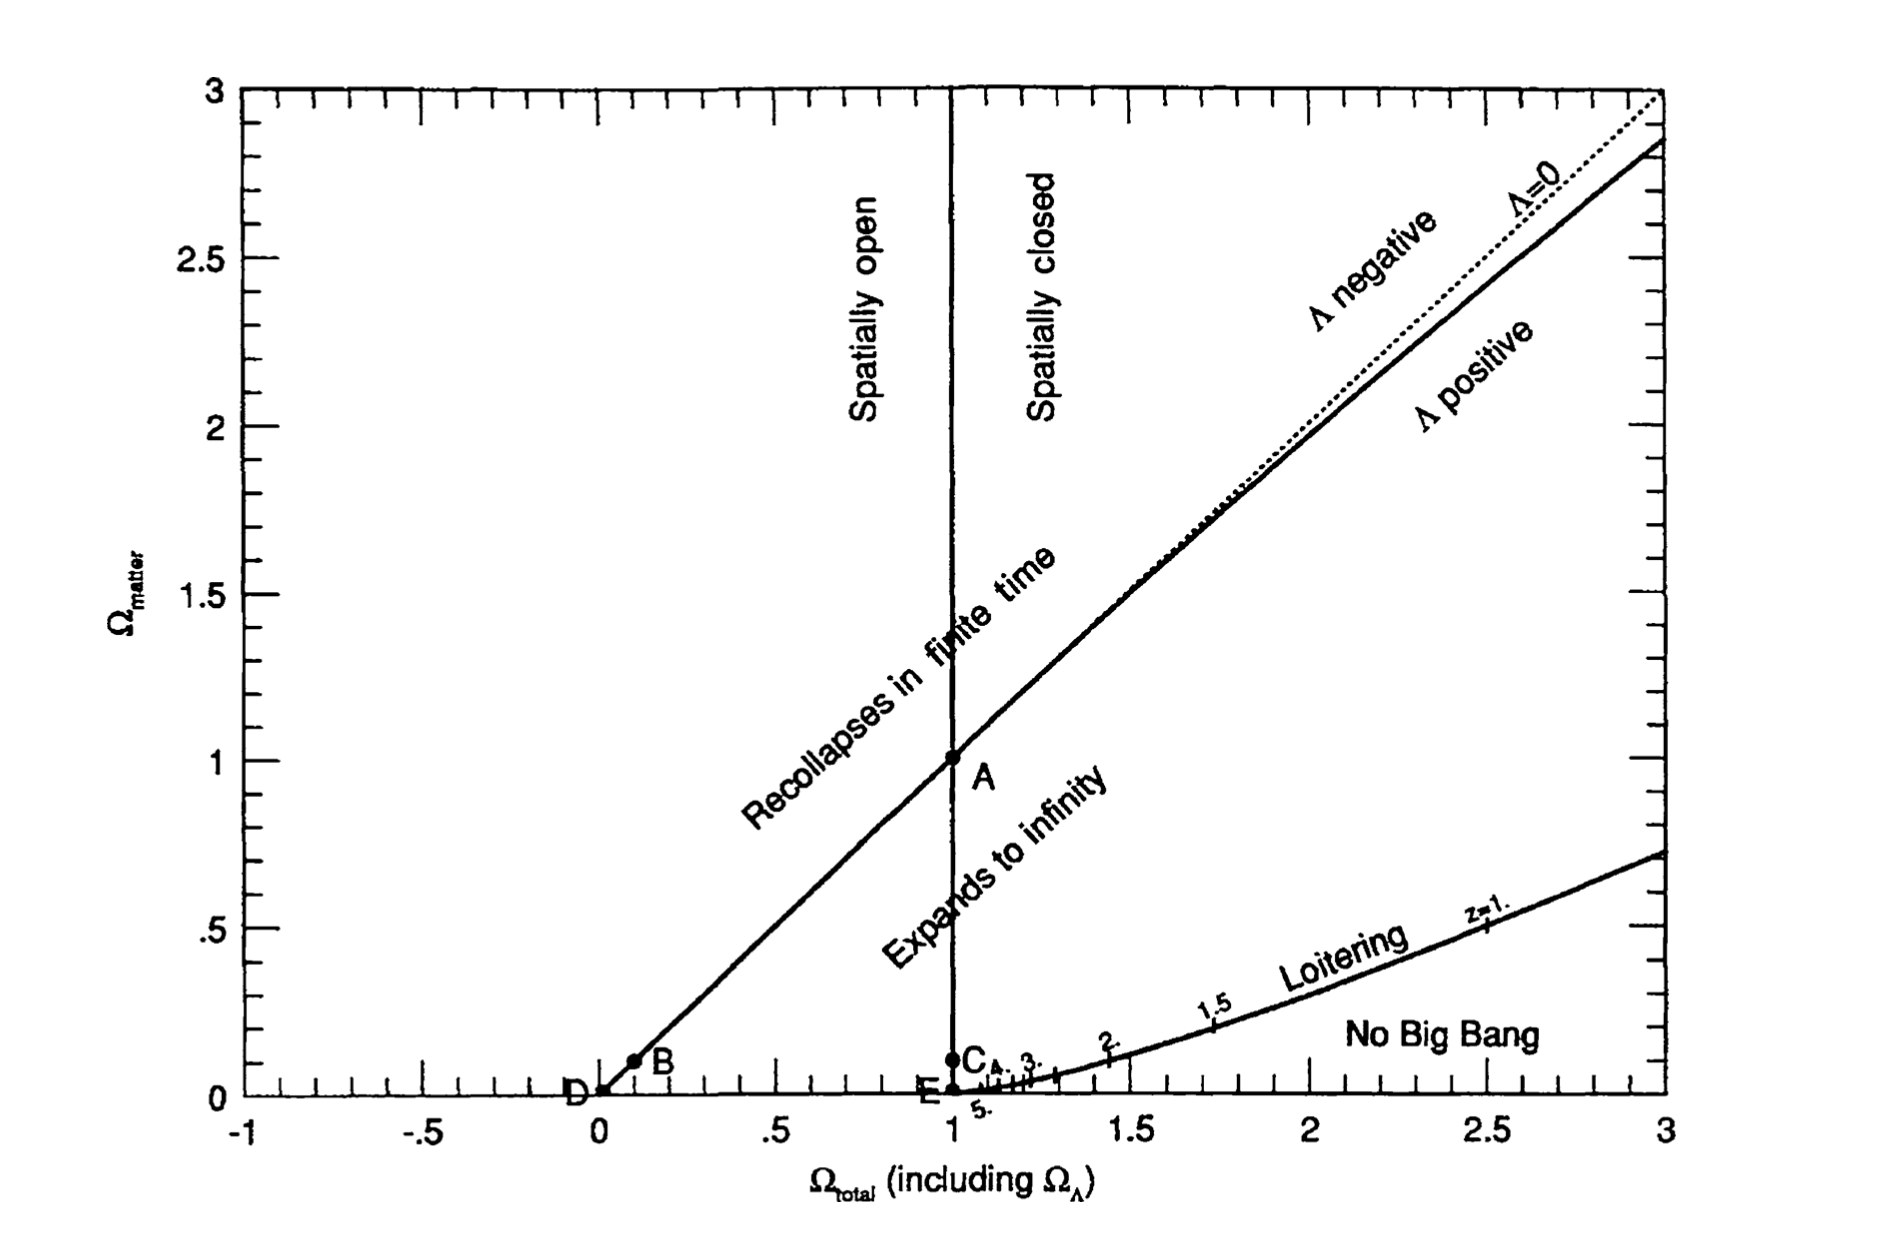
\includegraphics[width=16cm, height=11cm]{images/friedmann.png}
    \caption{Modelli di Friedmann}
    \label{fig:modelli}
\end{figure}
Nel ramo “A” l’universo si espande a partire da un’origine (big bang) nel passato e raggiunger\'{a} (eventualmente) uno stato stazionario nel futuro infinito. Nel ramo “B” l’universo si espande a partire da un valore definito di a nel passato infinito. Lo stato stazionario del modello di Eddington-Lemaitre \'{e} indicato da “C” ed \'{e} instabile perch\'{e} l’universo, se perturbato, si muove sul ramo B o A. Un modello “quasi” stazionario pu\'{o} essere quello in cui siamo nella fase asintotica $a(t)$ costante e quindi siamo partiti da un big bang ad un tempo infinito nel passato, ovvero il ramo A.\\
Parametri attuali:
\begin{equation}
     \begin{cases}
          q_0<0
         \\
         \Omega_0=0.3
         \\
         \Omega_{\Lambda 0}=0.7
     \end{cases}
\end{equation}
\subsubsection{Instabilit\'{a} del Modello di Einstein}
La regione piatta più essere simulata da un universo che rimbalza o da uno che si espande e poi collassa. Non \'{e} possibile sapere se ci si trova in un universo statico perch\'{e} potremmo essere in tutti quei punti. Gli stati stazionari appena visti sono instabili e richiedono un preciso fine tuning: cio\'{e} piccole variazioni di $\Omega_0$ e $\Omega_{\Lambda}$ portano alle soluzioni $\alpha<0$ oppure $\alpha>0$.
\subsubsection{Redshift per Modello di Universo senza Big Bang}
Se vivessimo in un universo che rimbalza non dovremmo vedere oggetti a $z>1.2$ ma dato che vediamo a $z=10$ allora non siamo in questa situazione.
\subsection{Distanza in cosmologia}
Riprendiamo il discorso fatto nella sezione "Redshift Cosmologico". Passo dalla variabile temporale a $z$ derivando la def. $1+z=\frac{1}{a}$. Sotto le ipotesi:
\begin{itemize}
    \item $w=0$
    \item $\Omega_{\Lambda0}=0$ ($\forall \Omega_0$ per ogni modello di Friedmann)
\end{itemize}
Ottengo:
\begin{equation}
    \int_{z}^{0}\frac{c dz'}{H_0 E^{\frac{1}{2}}}=f_k(r)
\end{equation}
Quindi dalla misura di $z$ posso stimare $r$ e viceversa dalla misura di $r$ posso stimare le costanti cosmologiche $\Omega_0$ e $\Omega_{\Lambda0}$.\\
Facendo le dovute sostituzioni ottengo la \textbf{formula di Mattig} \footnote{Che è la Legge di Hubble su larga scala, sono delle correzioni relativistiche}:
\begin{equation}
    r=\frac{2c}{H_0\Omega_0^2(1+z)}\left\{\Omega_0 z+(\Omega_0-2)[(\Omega_0 z+1)^{\frac{1}{2}}-1]\right\}
\end{equation}
Per determinare le costanti cosmologiche bisogna avere un indicatore di distanza e stare su grandi z.
\subsection{Relazione tipi distanza: coomovente vs angolare}
Voglio misurare la distanza coomovente $r$ (che non cambia), al tempo attuale $t_0$, di una sorgente a redshift $z$. L'emissione corrisponder\'{a} ad un tempo precente $t$, di conseguenza $d$ sar\'{a} cambiata.
\begin{equation}
     \begin{cases}
         D_A=\frac{r}{1+z}=ar
         \\
         D_A=\frac{d}{\theta}
     \end{cases}
\end{equation}
Dunque devo trovare una classe di oggetti di cui conosco le dimensioni $d$. Furono proposte le \textbf{Radiogalassie} poich\'{e} si pensava che la $d$ non variasse (Sbagliato!). Un altro problema \'{e} che $D_A$ a grandi z varia da col modello di Friedmann utilizzato (\textbf{decresce all'aumentare del parametro di densit\'{a}, dunque l'oggetto avr\'{a} un'apertura angolare maggiore}). Posso ricavare una misura di distanza da:
\begin{itemize}
    \item \textbf{CMB}: $D_A \sim \Omega_{k0}$ (err 1$\%$) \footnote{All'epoca del disaccoppiamento tra radiazione e materia le perturbazioni di densità che tendono ad oscillare (sotto la pressione di radiazione e l'instabilit\'{a} grav.), si congelano creando la mappo della CMB, le anisotropie hanno dimensioni diverse a seconda del momento in cui si sono formate. Dallo studio delle anisotropie si stima $\Omega_{k0}\sim 0$}
    \item \textbf{BAO}\footnote{Lo stesso fenomeno fisico del CMB provoca provoca una distribuzione disomogenea delle galassie su scale molto grandi, la Barionic Acoustic Oscillation}
    \item \textbf{Flusso}
\end{itemize}
\subsection{Flusso}
Ipotizzando \textbf{sorgente isotropa} e \textbf{universo in espansione}, la definizione di flusso deve cambiare, definiamo la \textbf{distanza di luminosit\'{a}}:
\begin{equation}
     \begin{cases}
         f=\frac{L(\nu_1)}{4 \pi D_L^2}
         \\
         D_L=(1+z)r=\frac{r}{a}
     \end{cases}
\end{equation}
L'andamento di $D_L(z)$ dipende dal modello di Friedmann che utilizziamo: diminuisce all'aumentare di $\Omega_0$. Osservo che con misure di $D_A$ e $D_L$ riusciamo ad avere una stima di $\Omega_0$ e $\Omega_\Lambda$.
\subsection{Brillanza buperficiale}
Ipotizzando \textbf{sorgente isotropa} e \textbf{universo in espansione}, la definizione di \textbf{Brillanza Superficiale} diventa:
\begin{equation}
    S_{oss}=\frac{S_{sorg}}{(1+z)^4}
\end{equation}
Ho dunque una diminuzione della Brillanza superficiale a  causa dell'espansione dell'universo. In magnitudini abbiamo invece l'opposto.
\begin{equation}
     \begin{cases}
        \mu=-2.5\log_{10}{S}+k
         \\
        \mu_{oss}=\mu_{sorg}+10\log_{10}{1+z}
     \end{cases}
\end{equation}
\subsubsection{Paradosso di Olbers}
Presupposti:
\begin{itemize}
    \item Universo infinito spazialmente e temporalmente
    \item Stelle disposte omogeneamente
\end{itemize}
Ipotesi che risolvono il paradosso:
\begin{itemize}
    \item L'universo esiste da un tempo finito
    \item L'universo è in espansione
\end{itemize}
Il fatto che il flusso sia $f \propto D^{-2}$ è compensato dal fatto che la densit\'{a} numerica di stelle cresca con $L= h \nu n V\propto D^2$, quindi il flusso osservato è costante. Perch\'{e} vediamo il cielo nero? La soluzione fu proposta da Edgar A. Poe che ipotizzo che sia finito, dunque ho delle los in cui posso non intercetto stelle, e in espansione, quindi la brillanza diminuisce in funzione di z.
Definiamo la \textbf{Correzione k}:
\begin{equation}
    f(\nu_0) \Delta\nu_0=\frac{L(\nu_1)\Delta\nu_1}{4\pi D_L^2}=\frac{L(\nu_0)\Delta\nu_0}{4\pi D_L^2}\frac{L(\nu_1)\Delta\nu_1}{L(\nu_0)\Delta\nu_0}\Delta_0
\end{equation}
Passando alle \textbf{Magnitudini Apparenti}:
\begin{equation}
    m_{\nu_0}=-2.5\log_{10}{\left\{\frac{L(\nu_1)\Delta\nu_1}{4\pi D_L^2}\Delta\nu_0\right\}}-2.5\log_{10}{\left\{\frac{L(\nu_1)}{L(\nu_0)}(1+z)\right\}}
\end{equation}
Definisco $k=\log_{10}{\left\{\frac{L(\nu_1)}{L(\nu_0)}(1+z)\right\}}$.
\subsection{Misura della distanza di luminosit\'{a}}
\begin{equation}
     \begin{cases}
        D_L=r(z)(1+z)=\frac{cz}{H_0}\left\{1+\frac{1}{2}(1-q_0)z\right\}
         \\
        m-M=5\log{\left\{ \frac{D_L}{10^{-6}}\right\}-5}
     \end{cases}
\end{equation}
La variabile $r$ la trovo dal calcolo di redshift con $ds^2=0$ sotituendo si ottiene il \textbf{Modulo di Distanza} in funzione di z. Osservo che aumentando la distanza della \textbf{candela standard} aumenta $m$ quindi \'{e} pi\'{u} debole il flusso, in modo opposto se sono in un universo con densit\'{a} critica minore allora il flusso diventa maggiore. A grandi $z$ entra in gioco il fattore $q_0$ che fa separare le curve:
\begin{itemize}
    \item $m-M$ e $\Omega_0$ sono inversamente proporzionali
    \item $m-M$ d al crescere di $\Omega_\Lambda0$ sono direttamente proporzionali
\end{itemize}
Il parametro $q_0$ allora lo stimo dalle SNIac\footnote{Stelle appartenenti a sistemi binari che esplodono con la massa costante di Chandrasekar ($M_{CH}=1.44 M_S$) raggiungendo il picco massimo di luminosit\'{a} a $10^{10} L_S$, la luminosit\'a equivalente ad una galassia.} misurando $z$ dagli spettri $m$ misurato da terra.\\
Ho due  problemi:
\begin{itemize}
    \item Vedere la SN al picco: monitoro il cielo a frequenza della settimana cerco le diff. di L.
    \item Non sono candele standard.
\end{itemize}
Tali oggetti non sono candele standard in quanto la luminosit\'{a} di picco dipende dalla metallicit\'{a} (quindi dal colore: rosse e metalliche, blu e poco metalliche) secondo la \textbf{relazione di Philips}. Risolvo il problema statisticamente attraverso \textbf{rinormalizzazione}, che mi porta ad avere le \textbf{curve di luce} sovrapponibili.
\subsubsection{Energia Oscura}
Alcuni cosmologi non credono che $q_0<0 \rightarrow \Omega_{\Lambda0}>0$, ma credono che esista un fluido chiamato \textbf{Energia Oscura} con densit\'{a} di energia positiva ma pressione negativa .
\begin{equation}
     \begin{cases}
        \rho_{\Lambda}=\frac{\Lambda}{4 \pi G}
        \\
        P_{\Lambda}=w\rho_{\Lambda}c^2; \quad w=-1
     \end{cases}
\end{equation}
\newpage
\section{Storia termica dell'universo }
L'universo primordiale è approssimabile ad un plasma di particelle \footnote{Protoni, elettroni, neutrini e fotoni.} libere\footnote{Trascuro le interazioni perch\'{e} l'Univ. non \'{e} cos\'{i} caldo.} estremamente caldo; dunque per  $t=0$ equazione di Einstein \'{e} singolare: temp. e densit\'{a} sono infinite. Ipotizzo valga il \textbf{limite termodinamico} \footnote{Considero additive le quantit\'{a} estensive, in quanto cio\'{e} la densit\'{a} non \'{e} cos\'{i} alta}. Definisco una \textbf{funzione di distribuzione} \footnote{Non ho dip. dalla posizione perch\'{e} considero U. omogeneo e isotropo} che all'\textbf{equilibrio cinetico} sar\'{a} una Fermi-Dirac o Bose-Einstein in base alle particelle in questione.
\begin{equation}
     \begin{cases}
        f(\textbf{p})=\frac{1}{\exp{\frac{E-\mu}{T}}\pm 1}
        \\
        \rho=\frac{g}{(2\pi)^3}\int E(\textbf{p}) f(\textbf{p})d\textbf{p}
        \\
        P=\frac{g}{(2\pi)^3}\int \frac{|\textbf{p}|^2}{3E} f(\textbf{p})d\textbf{p}
     \end{cases}
\end{equation}
\subsection{Asimmetria tra materia e antimateria}
Considero il \textbf{limite relativistico} $T >> m$, dunque i fotoni della CMB.
\begin{equation}
     \begin{cases}
        \rho_{BE}=\frac{\pi^2}{30}gT^4
        \\
        \rho_{FD}=\frac{7}{8}\frac{\pi^2}{30}gT^4
     \end{cases}
\end{equation}
\begin{equation}
    P=\frac{\rho}{3}
\end{equation}
\textbf{Teoricamnte}: abbiamo un miliardo di fotoni per ogni barione ($\eta=\frac{n_{b,0}}{n_{\gamma,0}}\sim 10^{-8}$). Dunque nell'universo primordiale \'{e} avvenuta la \textbf{rottura di simmetria}, di carica o parit\'{a}\footnote{Si studia attraverso la teoria dei campi}, si ha quindi materia in surplus rispetto ad antimateria. Dunque queste si annullano formando la CMB, ma rimane un po' di materia che costituisce l'univ. che vediamo.\\
\textbf{Osservativamente}: il rapporto tra barioni e fotoni non rispecchia i calcoli, infatti $\eta^{-1}\sim 10^{18}$. Lo possiamo anche vedere dall'entropia per barione. Questo \'{e} un problema aperto della cosmologia.
\subsection{Dipendenza delle grandezze termodinamiche delle specie}
Tramite normalizzazione per la $T_i$ delle grandezze termodinamiche, posso esprimere le variabili di riferimento attraverso una funzione della temperatura contenente il contributo di tutte le specie di particelle.
\begin{itemize}
    \item $u=\frac{E}{T_i}$
    \item $x_i=\frac{m_i}{T_i}$
    \item $y_i=\frac{\mu_i}{T_i}$
\end{itemize}
\begin{equation}
    g_*(T)=\sum_i \left\{\frac{T_i}{T}\right\}^4 g_i+\frac{7}{8}\sum_i \left\{\frac{T_i}{T}\right\}^4 g_i
\end{equation}
\subsubsection{Caso relativistico:}
\begin{equation}
     \begin{cases}
        \rho_{R}=\frac{\pi^2}{30}T^4 g_*(T)
        \\
        P_R=\frac{\rho_{R}}{3}
        \\
        S_{R}=\frac{4}{3}\frac{\pi^2}{30}T^3 g_*^S(T)
     \end{cases}
\end{equation}
\begin{equation}
    g_*^S(T)=\sum_i \left\{\frac{T_i}{T}\right\}^3 g_i+\frac{7}{8}\sum_i \left\{\frac{T_i}{T}\right\}^3 g_i
\end{equation}
Ipotizzando il sist. univ. \textbf{chiuso} \\footnote{In quanto non scambia energia e materia con l'esterno.} dunque tale espansione \'{e} \textbf{adiabatica} allora l'entropia \'{e} conservata e scala con il fattore di scala $S\propto a^3$ che implica $T\propto(1+z)$.
\subsubsection{Caso non relativistico:}
Sfruttando il \textbf{$1^o$ Principio della termodinamica} e la conservazione del tensore E-I si ha $T\propto(1+z)^2$.
\subsection{Disaccoppiamento}
La condizione per avere disaccoppiamento  tra due specie di particelle \footnote{Ovvero quando non hanno l'energia sufficiente per interagire.} si ha quanto il tempo scala di espansione supera quello di collisione $\tau_H < \tau_{coll}$.
\begin{equation}
    \begin{cases}
    \tau_{coll}\sim \Gamma^{-1}, \quad \Gamma=n\sigma|\textbf{v}|
    \\
    \tau_{H}\sim H^{-1}
    \end{cases}
\end{equation}
\subsubsection{Disaccoppiamento di neutrini}
(\'{E} di aiuto pensare al disaccoppiamento come all'istante in cui non ho pi\'{u} interazione tra alcune specie di particelle.)\\
\begin{equation}
    \begin{cases}
    e^{+} + e^{-}  \rightleftarrows \bar{\nu_e} + \nu_e 
    \\
    \nu_{e} + e^- \rightleftarrows \nu_{e} + e^-
    \\
    \nu_{e} + e^+ \rightleftarrows \nu_{\mu} + \mu^+
    \end{cases}
\end{equation}
I neutrini interagiscono \textbf{debolmente} con particelle relativistiche ad alte energie. Usiamo la \textbf{sezione d'urto di Fermi} ($\sigma \sim G_F^2T^2$) per determinare il \textbf{rapporto tra tasso di collisione ed espansione}. Siccome $n\propto T^3$ e $H \propto T^2 $\footnote{Considerando il modello EdS in cui impongo conservazione del T. E-I.} allora ottengo $\frac{\Gamma}{H}\propto \left\{\frac{T}{1 MeV}\right\}^3$. Nel momento in cui $T<1MeV$ allora i neutrini si disaccoppiano dalla materia relativistica iniziando una \textbf{fase di espansione libera} in cui $T\propto a^{-1}$, sono i \textbf{neutrini rielici} che costituiscono il \textbf{CNB} (Cosmic Neutrino Background\footnote{Come la CMB ora la loro energia \'{e} del ordine di $eV$.}).\\
Stimo ora la $T_{\nu 0}$ in funzione di $T_{\gamma 0}$. I fotoni raffreddandosi arrivano a $E<MeV$ non riusciranno pi\'{u} a creare coppie. Si perde l'equilibrio cinematico e la reazione sar\'{a} spostata verso \textbf{l'annichilazione} delle coppie e per conservazione dell'entropia\footnote{Poich\'{e} l'univ. si espande adiabaticamente.} questa si trasferir\'{a} ai fotoni incrementandone la temperatura. Dalla conservazione dell'entropia si ottiene $T_{\nu 0}=1.95K$. Tale risultato spiega perch\'{e} i neutrini rielici non siano ancora stati osservati, gli esperimenti sui neutrini astrofisici sono settati sul $MeV$. La densit\'{a} numerica è $n_{\nu}\simeq 110 N_{\nu} cm^{-3}$ dove $N_{\nu}=3$ sono i tipi di neutrini.
\begin{figure}[htp]
    \centering
    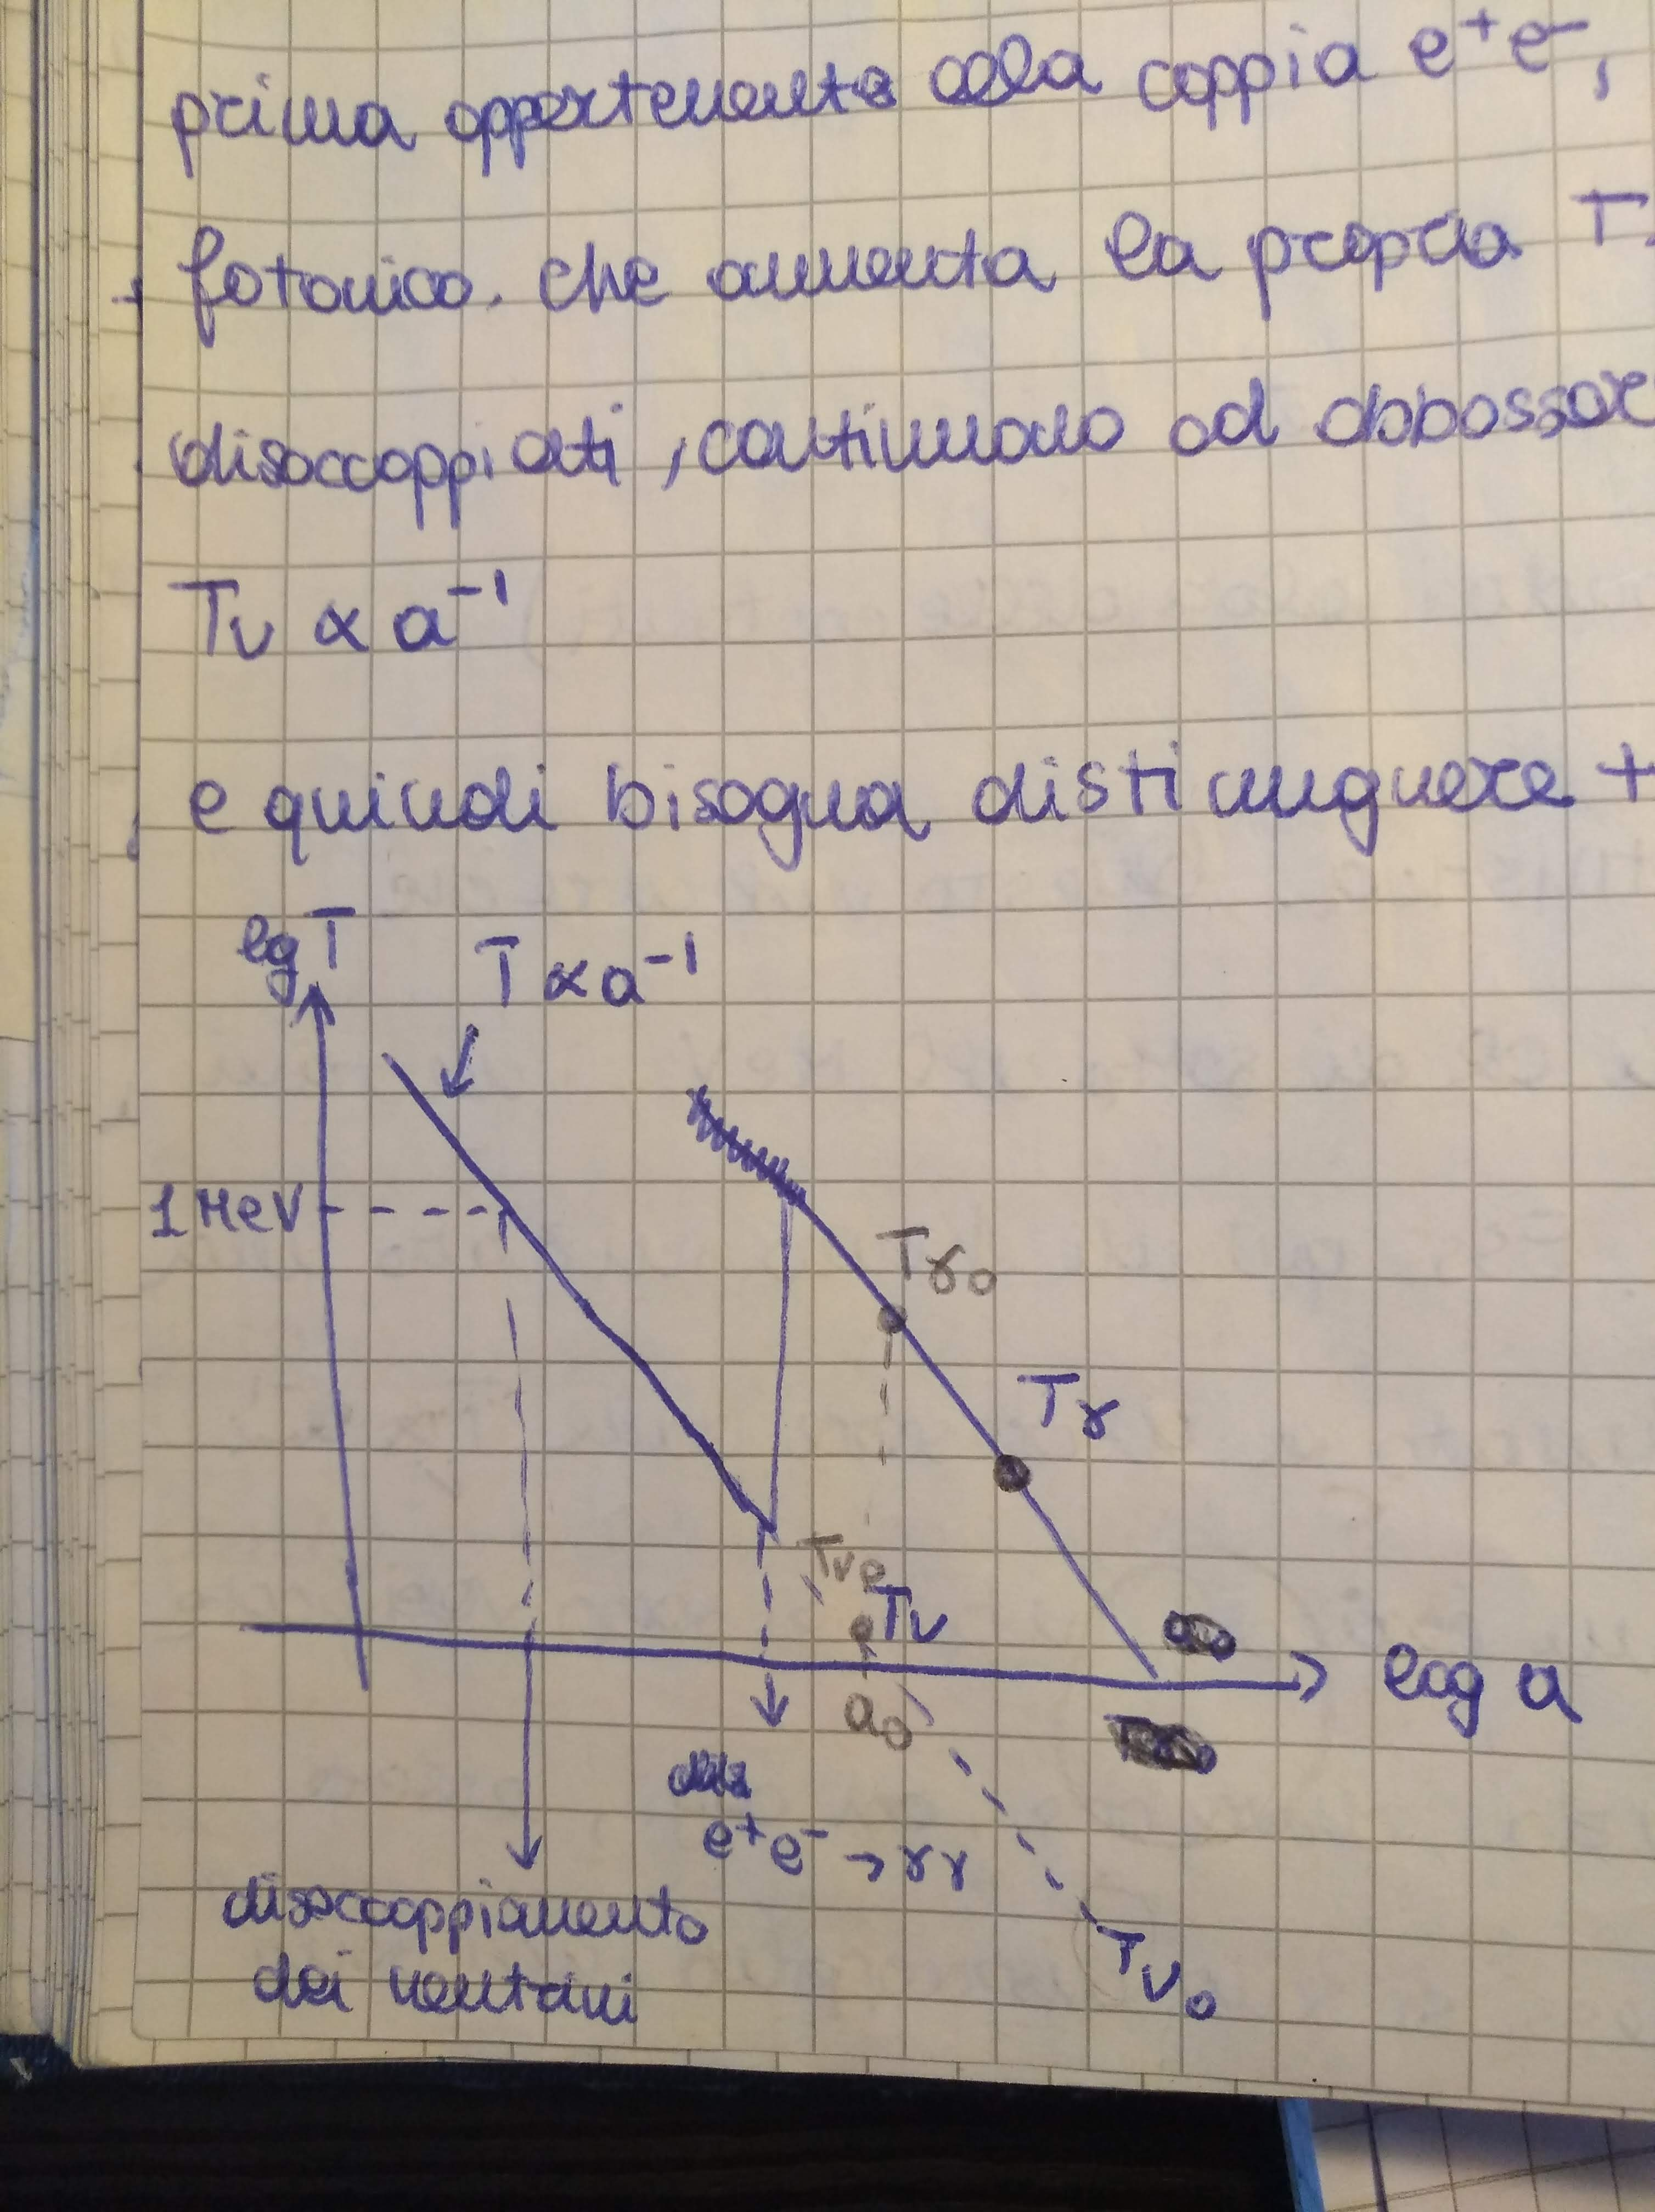
\includegraphics[width=10cm, height=7cm]{images/disaccoppiamento.jpg}
    \caption{Disaccoppiamento dei Neutrini.}
    \label{fig:neutrini}
\end{figure}
\subsection{Densit\'{a} energetica del fluido relativistico}
Dalle relazioni precedentemente trovate si ottiene che $\rho_{\nu}=68\% \rho_{\gamma}$ dunque non trascurabile nel parametro di denit\'{a} che risulta essere $\Omega_{\nu0}\sim 10^{-1}$ stimando $m_{\nu}=10eV$. Ma essendo la massa del neutrino $m_{\nu}=0.05eV$ risulta che non sia possibile che questi costituiscano la \textbf{materia oscura}.
\subsection{Epoca dell'equivalenza}
Questa fase \'{e} l'istante in cui la densit\'{a} della materia ordinaria eguaglia quella relativistica. Prima dominava la radiazione e poi da materia. Dalla cons. del T. E-I avevamo:
\begin{itemize}
    \item M. Ordinaria: $\rho a^3=k$
    \item M. Relativistica: $\rho a^4=k$
\end{itemize}
\subsection{Nucleosintesi cosmologica}
Uno dei motivi per cui il Big Bang \'{e} universalmente accettato come modello dominante \'{e} perch\'{e} riesce a spiegare le abbondanze di \textbf{elementi leggeri} con un elevata precisione.
\subsubsection{Premesse}
\begin{itemize}
    \item Osservazioni evidenziano che le abbondanze relative sono costanti per tutti gli oggetti astrofisici
    \item '20 Composizione solare: $74\% H, \quad 23\% He$
    \item '30 Scopro che le reazioni termonucleari producono elementi chimici.
    \item '40 Gamov-Bethe-Alpher ipotizzano che il Big Bang produce elementi leggeri e le stelle quelli pesanti.
    \item '50 Scopro che le stelle producono elementi pesanti attraverso le reazione termonucleari.
    \item PB: Mancanza di elio e deuterio.
\end{itemize}
\subsubsection{Aspetti quantitativi}
Per descrivere la Nucleosintesi \'{e} necessario capire l'accoppiamento tra radiazione e materia in presenza di interazioni che variano il numero di particelle che ne prendono parte. Considero l'epoca in cui $1MeV<E<1GeV$ (limite non relativistico) in cui abbiamo processi di \textbf{interazione debole}:
\begin{equation}
    \begin{cases}
    n \rightleftarrows p + e^{-} + \bar{\nu_e}
    \\
    \nu_{e}+n \rightleftarrows p +e^{-}
    \\
    e^{+} + n\rightleftarrows p + \bar{\nu_e}
    \end{cases}
\end{equation}
E i \textbf{processi di scattering}:
\begin{equation}
    \begin{cases}
    e^{-} + \gamma \rightleftarrows e^{-} + \gamma
    \\
    e^{+} + \gamma \rightleftarrows e^{+} + \gamma
    \end{cases}
\end{equation}
Stiamo considerando queste reazioni all'\textbf{eq. cinematico} e \textbf{termodinamico} quindi a densit\'{a} e temperature tali da garantire reversibilit\'{a}. Considerando particelle non relativistiche la loro funzione di distribuzione sar\'{a} una Maxwell-Boltzmann. Dalla prima interazione debole si ottiene $\frac{n_n}{n_p} = \exp{-\frac{Q + \mu_n -\mu_p}{T}}$ tale che:\\
\begin{equation}
    \begin{cases}
    T \sim 1MeV \rightarrow \frac{n}{p}=1
    \\
    T < 1MeV \rightarrow \frac{n}{p}<1
    \end{cases}
\end{equation}
Per $T < 1MeV$ abbiamo il disaccoppiamento dei neutrini allora l'interazione sar\'{a} spostata verso la protonizzazione. Considerando la seconda interazione debole avremo $\frac{n}{p} \simeq \exp{-\frac{Q }{T}}$. All'epoca in cui i neutrini si disaccoppia anche i protoni e i neutroni escono dall'equilibrio, la frazione si congela a $\frac{n}{p} \simeq 0.27$, dunque si hanno 4 neutroni per protone. La maggior parte dei neutroni si lega formando elio mentre gli altri decadono ($\tau_n\sim 15$ min.) diminuendo il rappoto $\frac{n}{p}$.\\
\begin{figure}[htp]
    \centering
    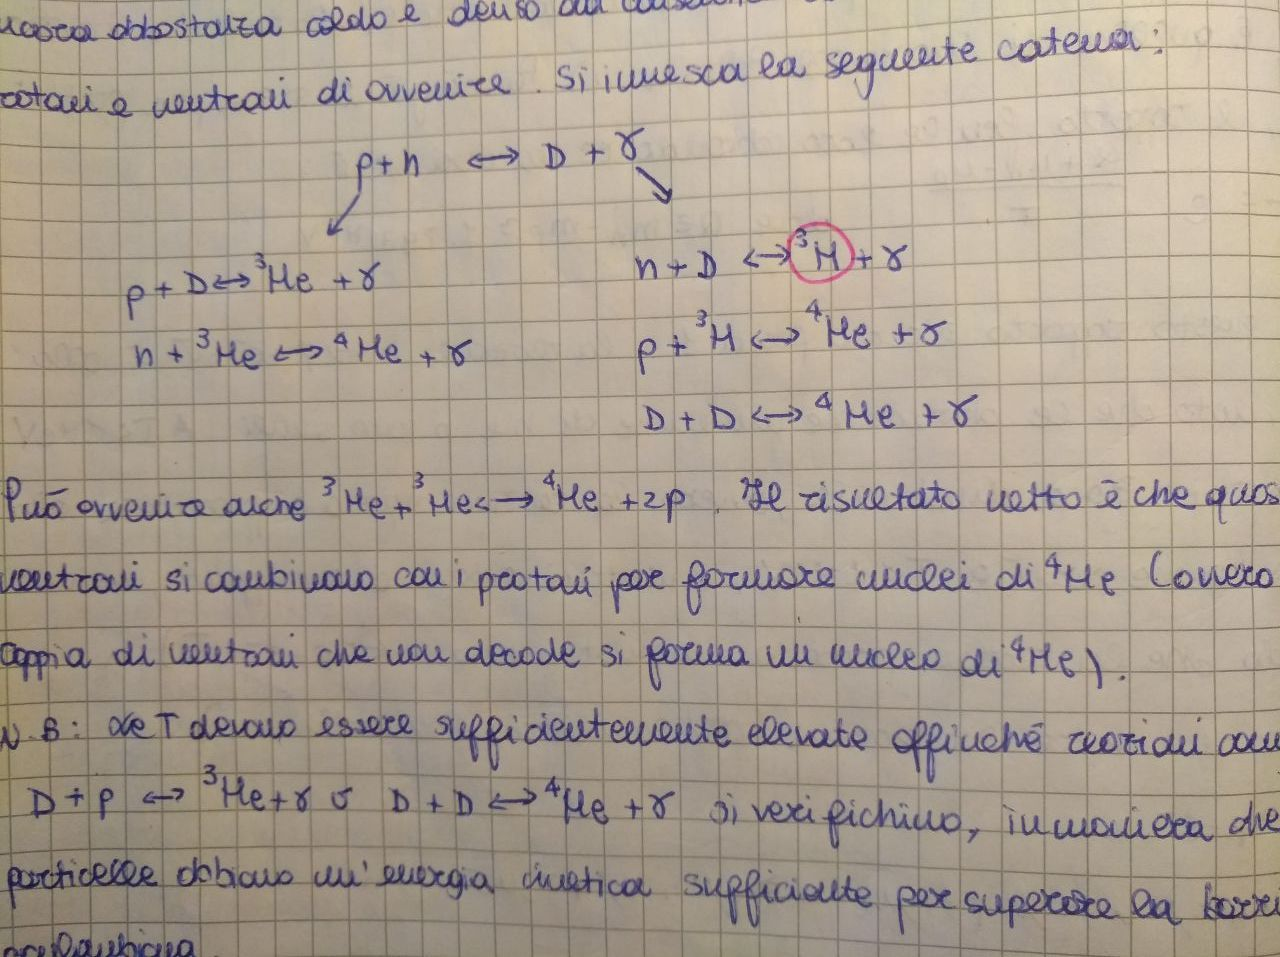
\includegraphics[width=10cm, height=7cm]{images/catena.jpeg}
    \caption{Catena di Interazioni.}
    \label{fig:Int}
\end{figure}
Per arrivare alla sintesi dell'elio bisogna passare dalla sintesi del deuterio $E_D=2.23$ che a $T \sim 1MeV \sim 10^9 K$ per il gas di fotoni viene completamente distrutto \footnote{La Planckiana associata alla $T \sim 1MeV$ ha una coda che contiene fotoni a temperatura sufficiente per scindere tutta la popolazione di deuterio presente.}; dunque per avere elio bisogna aspettare che la temperatura dell'universo si abbassi di un fattore $10K$ per permettere al deuterio di sopravvivere. Sfruttando le relazioni $t \propto a^2 \propto T^2$, in ipotesi di EdS in universo dominato dalla radiazione, stimiamo l'istante di tempo in cui si verificano queste interazioni $t\simeq 100 s$. Mentre la durata della nucleosintesi \'{e} $Delta_{BBN}\sim 15 min$, si nota che nel tempo la temperatura e il numero di neutroni scendono progressivamente \footnote{La BBN \'{e} influenzata dall'espansione e dalla densit\'{a} dell'universo.}.
\subsection{Abbondanza di elio}
Considerando che:
\begin{itemize}
    \item Il tempo di inizio della BBN $t_s\simeq 400 s$ \footnote{Che corrisponde a $T\sim0.1 MeV$ mentre dovremmo utilizzare $t\sim 6.25 s$ che corrisponde a $T\sim0.8 MeV$, ma va bene perch\'{e} \'{e} una differenza trascurabile.}
    \item All'inizio della nucleosintesi $\frac{n}{p}=0.1265$.
    \item Il $\tau_n = 614s$ \footnote{Fosse minore si avrebbero meno neutroni e dunque elio.}
\end{itemize}
Allora stimiamo l'abbondanza di elio essere $Y=\frac{m_{He}}{m_H+m_{He}}=0.23$. La fisica che determina l'abbondanza di elio \'{e} diversa dagli altri elementi in quanto \'{e} termodinamica e determinata da $\frac{n}{p}$ al tempo del disaccoppiamento dei $\nu$. In aggiunta all'elio vengo prodotti altri elementi leggeri come He3 H3 e Li7, le cui abbondanze dipendono dalla rapidit\'{a} delle reazioni di interazione per formare i nuclei.\\
Differenze tra BBN:
\begin{itemize}
    \item BBN: esplosiva e rapida
    \item SN: a eq. termodinamico su tempi scala molto lunghi
\end{itemize}
\subsection{Abbondanza elementi leggeri}
Grafico le abbondanze di elemeneti leggeri in funzione di $\eta$ densit\'{a} numerica barionica per unit\'{a} di densit\'{a} numerica fotonica.\\
\begin{figure}[htp]
    \centering
    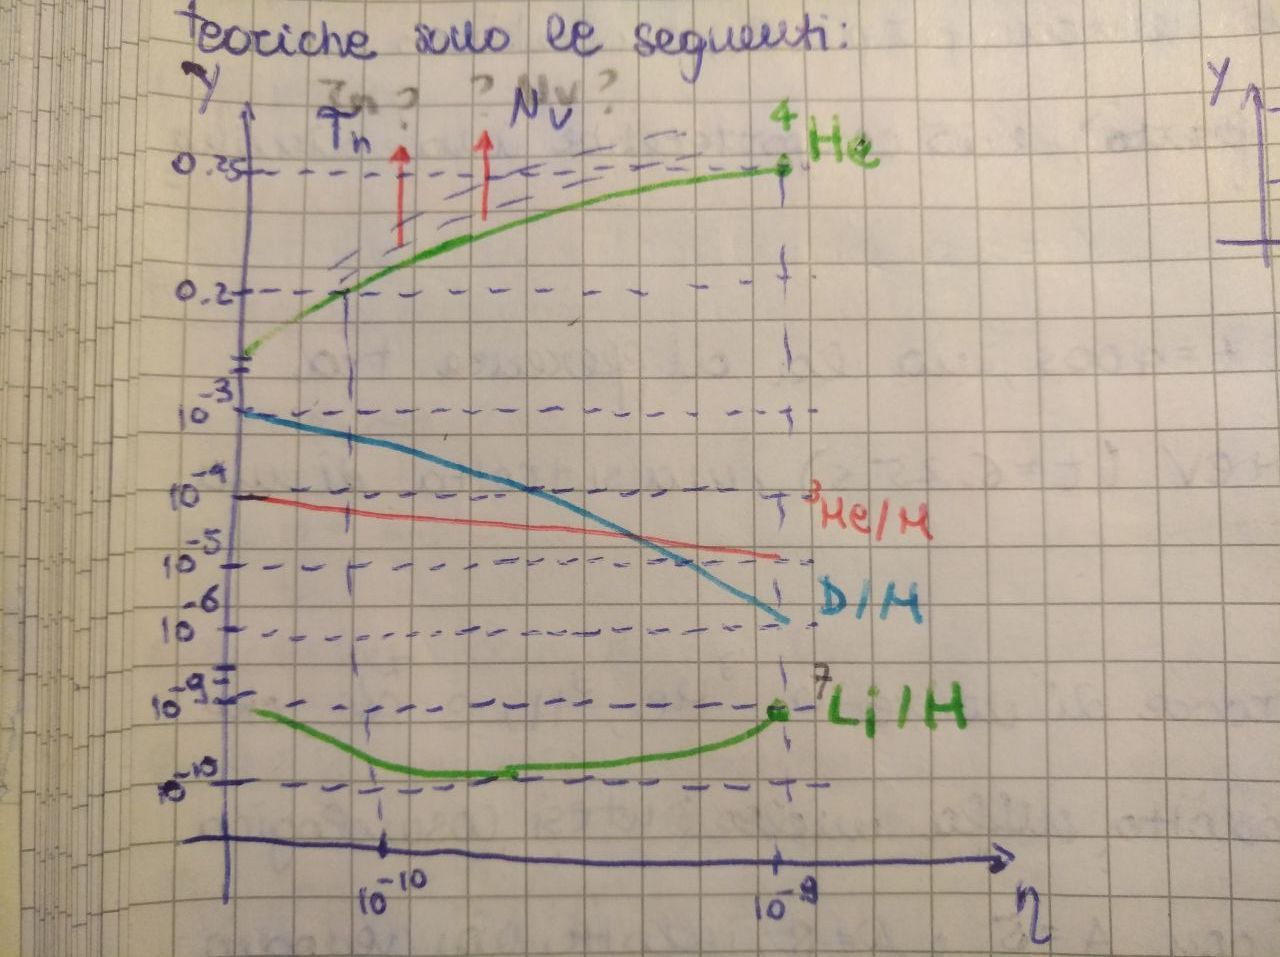
\includegraphics[width=9cm, height=6cm]{images/leggeri.jpeg}
    \caption{Abbondanza di Elementi Leggeri.}
    \label{fig:leggeri}
\end{figure}
\textbf{Oss1:}  L'abbondanza di \textbf{elio} pu\'{o} aumentare \footnote{L'aumento \'{e} esiguo dell'ordine del 5$\%$} due motivi:\\
\begin{enumerate}
\item  Aumentando i $\nu$ aumenta la densit\'{a} di energia dell'universo dunque rallentiamo l'espansione.
\item Aumentando il tempo di decadimento $\tau_n$.
\end{enumerate}
\textbf{Oss2:} L'abbondanza di \textbf{deuterio} decresce di 3 ordini di grandezza.\\
\textbf{Oss3:} L'abbondanza di \textbf{litio} decresce nella prima parte perch\'{e} funge da catalizzatore per la sintesi di elio e poi aumenta poich\'{e} viene sintetizzato.\\
Fissando degli estremi per il parametro $\eta$ fisso un intervallo per  $\Omega_b$ da cui ricavo il limite superiore $\Omega_b<0.03$: dunque la densit\'{a} di barioni \'{e} circa il $3\%$ della densit\'{a} critica. Il risultato \'{e} coerente con la stima di $\Omega_0$ ottenuta attraverso metodo dinamico sugli ammassi di galassie \footnote{ $3\%$ materia ordinari, $15\%$ plasma e il restante \'{e} materia non luminosa}, quindi se la stima \'{e} corretta, allora il modello di Big Bang caldo \'{e} valido e dobbiamo ammettere l'esistenza di una materia non barionica non luminosa. L'unica particella nota che potrebbe costituire la materia oscura sarebbe il \textbf{neutrino} \footnote{ Dato che si \'{e} disaccoppiato non viene considerato come materia barionica.}, ma in tal caso le strutture cosmiche avrebbero un altra forma rispetto a quella attuale.
\subsection{Misura delle abbondanze degli elementi leggeri}
Le abbondanze dei leggeri dipendono dal parametro cosmologico $\Omega_b$, per stimarlo correttamente devo eliminare la contaminazione da processi astrofisici.
\subsubsection{Stima dell'abbondanza di He4 primordiale}
\begin{itemize}
\item L'elio  \'{e} prodotto nel nucleo di stelle nella MS
\item Attraverso gli spettri possiamo determinare l'elio presente nella fotosfera che per\'{o} deriva dall'inquinamento della nube protostellare da stelle ormai morte
\end{itemize}

Dall'analisi delle \textbf{fotosfere di stelle di Pop II} ($Z\propto 10^{-4}-10^{-3}$) si studia l'andamento di Y in funzione di Z , e successivamente facendo l'estrapolazione a $Z=0$.\footnote{Sarebbe pi\'{u} preciso studiare direttamente le stelle di PopIII ($Z=0$) ma essendo gi\'{a} morte non \'{e} possibile.}
\subsubsection{Stima dell'abbondanza di D primordiale}
\begin{itemize}
\item L'abbondanza di deuterio \'{e} estremamente sensibile alla variazione di $\Omega_b$
\item Viene distrutto nella nucleosintesi stellare in quanto catalizzatore per elio, dunque quello che vediamo ha origine primordiale
\end{itemize}
Esistono due modi per stimare l'abbondanza di deuterio:
\begin{enumerate}
\item \textbf{ISM}: da cui misuriamo $\frac{D}{H}\sim (3-4)10^{-5}$ \footnote{Non \'{e} detto che il mezzo interstellare non sia stato affatto inquinato.}
\item \textbf{IGM}: dallo studio l'intensit\'{a} degli spettri dei quasar\footnote{Li scelgo perch\'{e} sono lontani quindi attraversano molto IGM.} (la cui densit\'{a} picca $z\sim 2$ ) determino,  in base alla profondit\'{a} della riga di assorbimento (Li$\alpha$), l'abbondanza di deuterio.
\end{enumerate}
I due metodi presentano risultati in accordo e inoltre la distribuzione di deuterio ha un alto grado di isotropia, questo fa pensare che sia di origine cosmologica.
\subsubsection{Stima dell'abbondanza di He3 primordiale}
Anche He3 \'{e} prodotto e distrutto nelle stelle dunque meno affidabile per la stima di $\Omega_b$. Pu\'{o} essere misurato nelle regioni HII (idrogeno ionizzato) $\frac{He3}{H}\sim (1-2)10^{-5}$.
\textbf{Stima dell'abbondanza di Li7 primordiale}
Il Li7 \'{e} un elemento fragile sintetizzato nelle stelle e distrutto da molto fenomeni astrofisici:
\begin{itemize}
\item Dalle stelle in quanto \textbf{catalizzatore} di He4
\item Per \textbf{spallazione} : collisione coi raggi cosmici
\item Per collisione col \textbf{ISM freddo}
\end{itemize}
L'abbondanza di Li7 primordiale si stima dalle stelle di \textbf{Pop II massicce} \footnote{Non uso stelle di massa inferiore a quella del sole perch\'{e} hanno inviluppo convettivo che porta il Li7 in profondit\'{a} ad alimentare le reazioni del nucleo alterandone le quantit\'{a}.} e risulta essere $\frac{Li7}{H}\sim 1.10 \cdot 10^{-10}$. Risulta non essere completamente in accordo con le previsioni del modello HBB: \'{e} circa 3 volte pi\'{u} basso. Questo si pensa essere dovuto a ragioni astrofisiche:
\begin{enumerate}
\item Difficolt\'{a} delle misure sperimentali
\item Parte del Li7 potrebbe essere stato distrutto dalle \textbf{novae} in sistemi binari dalle \textbf{reazioni picnonucleari} \footnote{La temperatura non \'{e} cos\'{i} alta da far avvenire reazioni termonucleari.} causate dall' aumento repentino della densit\'{a} nel violento scambio di materia tra le compagne
\end{enumerate}
Una ragione cosmologica invece:
\begin{enumerate}
\item Il modello di Universo usato \'{e} omogeneo e isotropo mentre le piccole disomogeneit\'{a} potrebbero spiegare questa discrepanza
\end{enumerate}
\subsubsection{Conclusioni}
Le abbondanze osservate di elementi leggeri primordiali risultano essere in buon accordo con le previsioni della nucleosintesi cosmologica. Questo fornisce un limite a $\Omega_b=0.03$ contro  $\Omega_0=0.3$; quindi gran parte della materia deve essere non barionica.
\subsection{Epoca della ricombinazione}
Siamo in un ambiente dove $\frac{H}{He}\sim 12$ ($X\sim 74\%, \quad
Y\sim 25\%$) a $T=(0.04 - 0.05)MeV$, per cui \'{e} possibile che avrei la seguente interaz.:
\begin{equation}
       e^{-} + p \rightleftarrows H + \gamma
\end{equation}
La reazioine \'{e} all'equilibrio per $E_{\gamma}=13.6 eV$, l'energia di prima ionizzazione di H, mentre per $E_{\gamma}<13.6 eV$ si ha \textbf{ricombinazione}. L'\textbf{eq. di Saha} determina il grado di ionizzazione dell'epoca di ricombinazione:
\begin{equation}
\frac{1-X_e}{X_e^2}=\frac{4\sqrt{2} \zeta(3)}{\sqrt{\pi}}\eta \left\{ \frac{T}{m_e}\right\}^{\frac{3}{2}} \exp{\frac{B}{T}}
\end{equation}

Dove $B=m_p+m_e-m_H$ energia di legame e $X_e=\frac{n_p}{n_b}$: se $X_e=0$ ho \textbf{ric. totale}, se $X_e=1$ ho \textbf{ionizzaz. totale}. Siccome $T \propto 1+z$ anche  $X_e \propto z$. Considero la distrib. di \textbf{ MB non collisionale}.
\begin{figure}[htp]
    \centering
    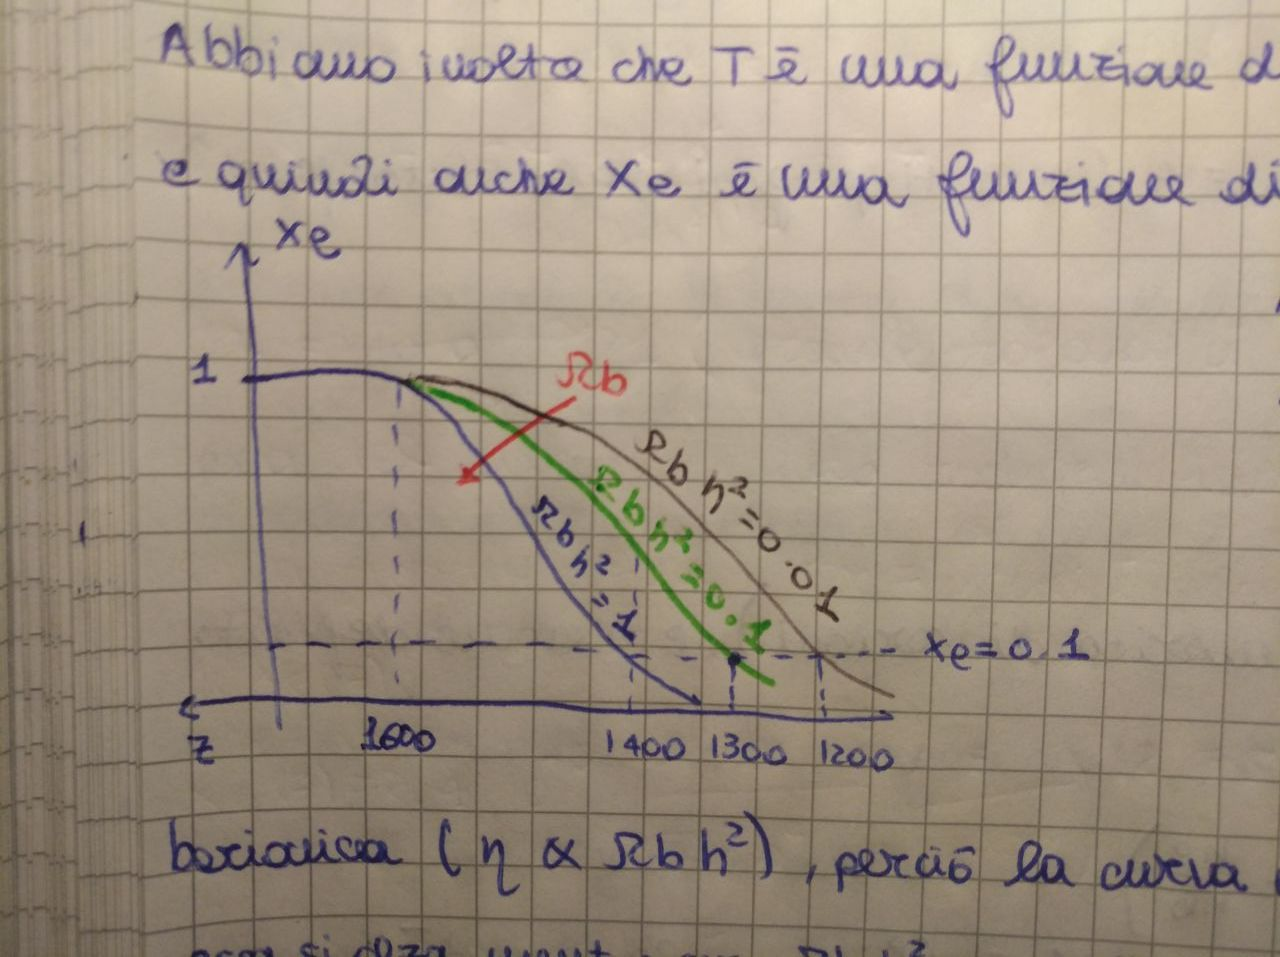
\includegraphics[width=9cm, height=6cm]{images/ric1.jpeg}
    \caption{Saha Non Collisionale}
    \label{fig:ric1}
\end{figure}
Osservazioni:
\begin{enumerate}
\item  $z \uparrow \rightarrow X_e=1; \quad z \downarrow \rightarrow X_e=0 $
\item $X_e$ e $\Omega_b$ sono inversamente prop. ($\eta \propto \Omega_b h^2$): la quantit\'{a} di materia decelera l'espansione favorendo la ricombinaz.
\item Se per $ X_e<0.1$ H \'{e} totalmente ric. allora $T_{ric}=3276 K$ 
\end{enumerate}
Invece, considerando lo \textbf{scatterning Thomson}\footnote{Lo scattering T. diminuisce coll'espansione dell'univ., fino ad arrivare al disaccoppiamento tra radiazione e materia.}, che porterebbe a ionizzaz. di H, avrei una \textbf{distrib. MB collisionale}:
\begin{figure}[htp]
    \centering
    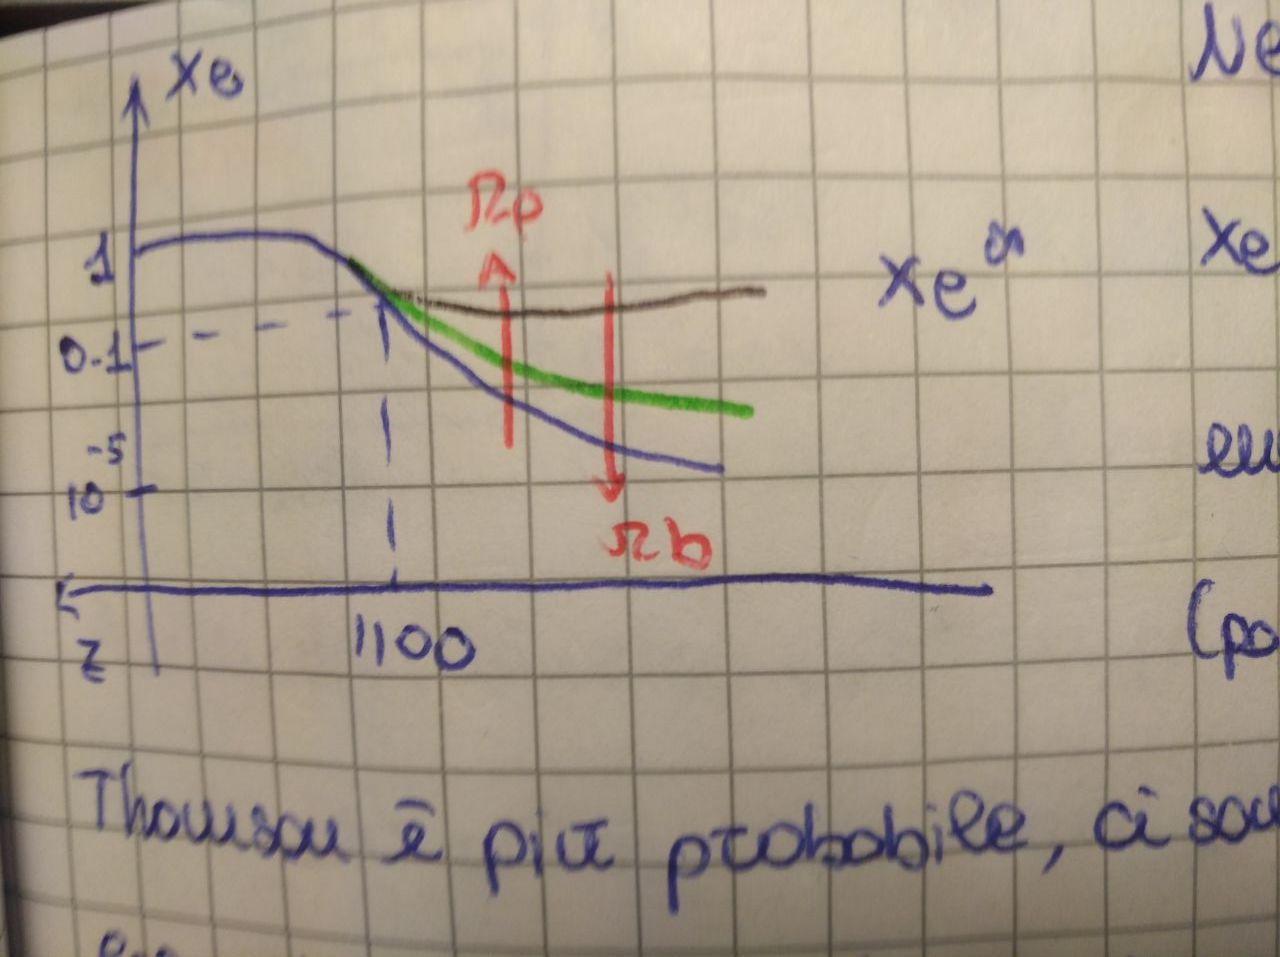
\includegraphics[width=9cm, height=6cm]{images/ric2.jpeg}
    \caption{Saha Collisionale.}
    \label{fig:ric2}
\end{figure}
Osservazioni:
\begin{enumerate}
\item \textbf{Freeze-Out}: congelamento della Fraz. di Ioniz., le curve non vanno a zero a causa dell'espansione il fmp diverge., la probabilit\'{a} di ricomb. diminuisce
\item Nella regione asintotica $X_e$ e $\Omega_0$ sono direttamente pro. in quanto l'espansione lenta aumenta la prob. di avere scattering T.
\end{enumerate}
Calcoli pi\'{u} approssimati ci danno la $X_e$ di \textbf{freeze-out}: $X_e^{\infty}=2.7\cdot 10^{-5} \frac{(\Omega_0 h^2)^{\frac{1}{2}}}{\Omega_0 h^2}$.
\subsection{Disaccoppiamento radiazione-materia}
A grandi z l'universo \'{e} \textbf{otticamente spesso} $\tau \simeq 0.37(\frac{z}{1000}^{14.25})$ dunque non lo possiamo indagare attraverso onde EM in quanto elettroni e fotoni fanno scattering Thomson. L'interazione diminuisce con l'espandersi dell'univ. e a $z=1070$ abbiamo la \textbf{superficie di ultimo scatternig} che libera i fotoni delle CMB: abbiamo una \textbf{barriera di fotoni} che non ci permette di vedere a z pi\'{u} grandi.\\
Considerando l'univ. come fluido relat. $T\propto a ^{-1}$ definiamo le seguenti epoche:
\begin{figure}[htp]
    \centering
    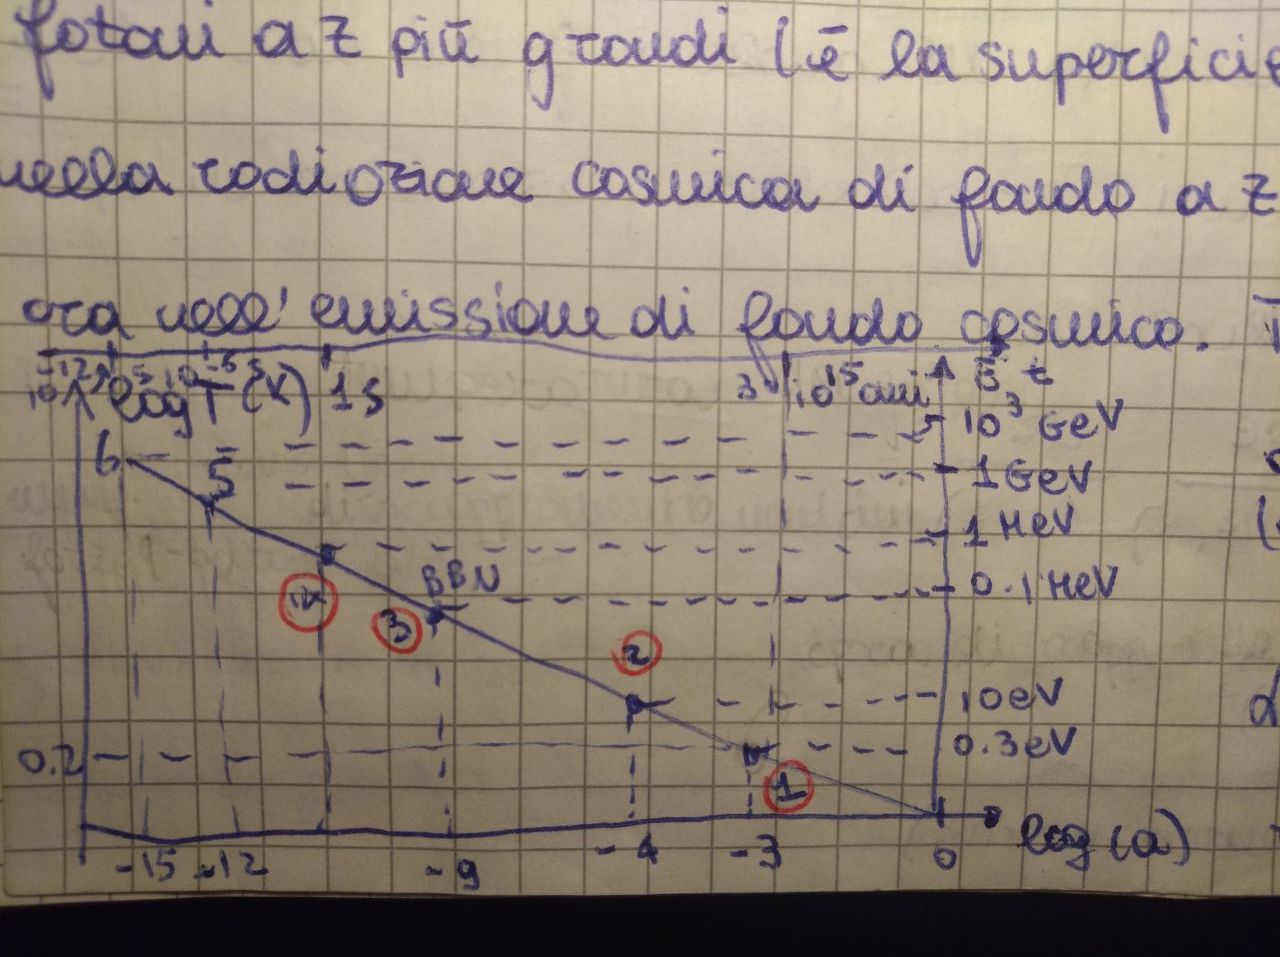
\includegraphics[width=9cm, height=6cm]{images/storia.jpeg}
    \caption{Storia termica dell'universo primordiale.}
    \label{fig:storia}
\end{figure}
\begin{enumerate}
\item Disaccoppiamento radiazione-materia ($T=0.3 eV$)
\item Eq. radiazione materia ($T=10 eV$)
\item BBN ($T=0.1 MeV$)
\item Annichilazione positroni-elettroni ($T=0.5 MeV$)
\item Disaccoppiamento neutrini  ($T=1 MeV$)
\item Transizione quark-adroni  ($T=1 GeV$)
\item Unificazione forse elettrodeboli  ($T=10^3 GeV$)
\item GUT: \textbf{periodo del deserto} le forze elettrodeboli e forti si unificano  ($T=10^{14}-10^{15} GeV$)
\item Inflazione ($t<t_P=10^{-43}s$\footnote{Le particelle iniziano ad auto gravitare. Per calcolare il tempo di Planck metto insieme il collasso in caduta libera e il principio di indeterminazione. }, $T_P\approx 10^{32}$, $E_P\sim 10^{19}GeV$)
\end{enumerate}
Osservazioni:
\begin{itemize}
\item Per $E =1-10 TeV$ studio la fisica con LHC
\item  Per $E >10 TeV$ non esistono esperimenti, ma ho la QFT come teoria
\item Se voglio studiare l'inflazione necessito di una teoria quantistica della gravit\'{a}
\item Da 1 a 4 \textbf{era radiativo}
\item Da 6 e 7 \textbf{era leptonica}
\end{itemize}
\subsection{Epoca inflattiva}
Dopo il \textbf{periodo del deserto cosmico}, in cui non identifichiamo particelle note, abbiamo l'epoca inflattiva che si estende per un arco di tempo $10^{-34}s<t<10^{-32} s$. Nella suddetta si introducono delle \textbf{transizione di fase} con cui possiamo risolvere i problemi del modello HBB. Basta traslare il concetto di energia libera dalla termodinamica alla QFT: qui si ha il potenziale di interazione in funzione del campo scalare \footnote{Che ha come componente fisica il bosone di Higgs.}. Teniamo sempre presente che il sistema fisico tende alla configurazione a energia minima.
\begin{figure}[htp]
    \centering
    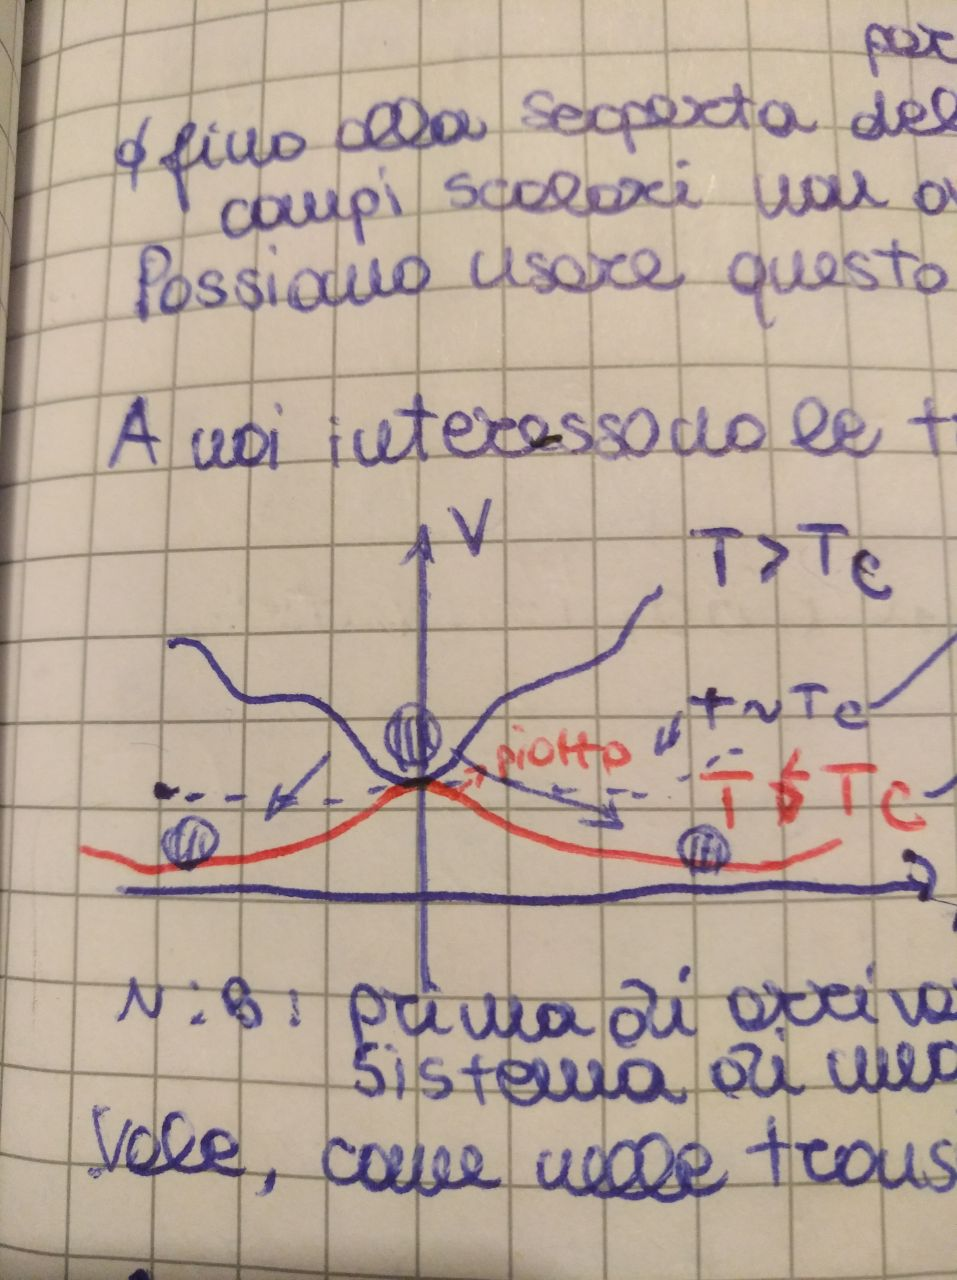
\includegraphics[width=9cm, height=9cm]{images/sombrero.jpeg}
    \caption{Potenziale di interazione a sombrero.}
    \label{fig:sombrero}
\end{figure}
Il potenziale effettivo varia in funzione della temperatura. Dunque analizziamo i casi:
\begin{enumerate}
\item $T>T_c$ il potenziale ha un minimo assoluto in $\phi=0$
\item $T \sim T_c$  il sistema permette di assumere valori di $\phi$ pi\'{u} grandi (transizione di fase del $1^°$ ordine)
\item $T<T_c$ in cui il minimo iniziale si trasforma in un massimo relativo, il sistema tende a due nuovi minimi (transizione di fase del $2^°$ ordine)
\end{enumerate}
Si verifica una \textbf{rottura di simmetria} che in QFT si esprime tramite una transizione di fase del $2^°$ ordine (GUT). Durante la transizione di fase abbiamo una perdita di energia che pu\'{o} interpretarsi come \textbf{calore latente} che fluisce nel sistema circostante.
\subsection{Problemi del modello HBB}
Il modello di big Bang caldo risultava avere delle criticit\'{a} prima del tempo di Planck, che verranno risolte dall'introduzione delle transizioni di fase nell'epoca inflattiva negli inizi degli anni '80.
\subsubsection{Problema dell'orizzonte}
Confrontando gli spettri di regioni dell'universo, sulle scale del CMB, si nota che regioni dell'universo che non dovrebbero essere mai entrate in contatto, causalmente non connesse \footnote{A causa di una distanza tra esse superiore a quella che ha potuto percorrere la luce nel tempo stimato dall'evento iniziale del Big Bang.}, hanno la stessa temperatura $T=2.7K$. Anche se l'universo non ha avuto il tempo di \textbf{termalizzare}.
\begin{figure}[htp]
    \centering
    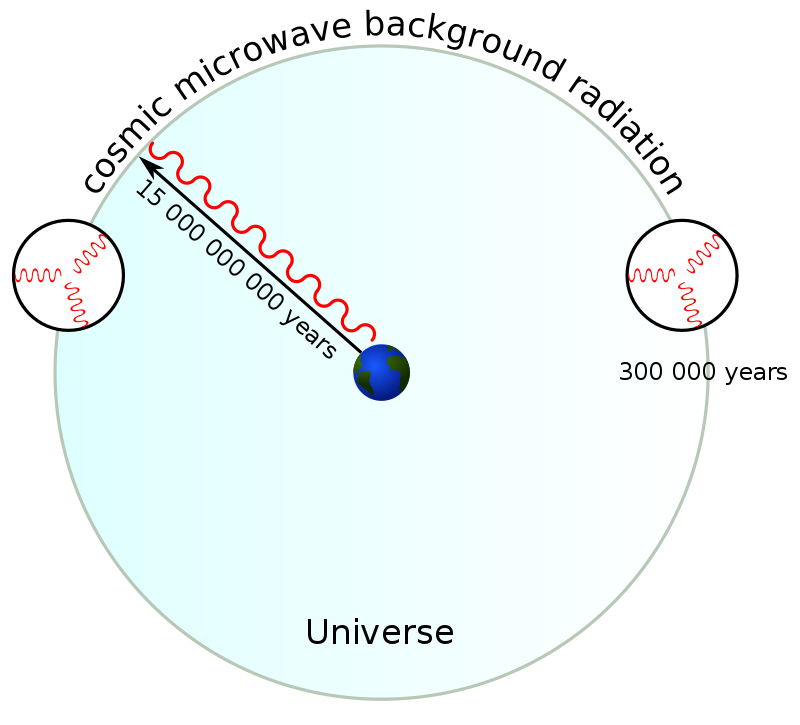
\includegraphics[width=7cm, height=7cm]{images/orizzonte.png}
    \caption{Problema dell'orizzonte cosmologico.}
    \label{fig:orizzonte}
\end{figure}
\begin{equation}
    \begin{cases}
   r_H\sim \frac{2c}{H_0 \Omega_0^{\frac{1}{2}} (1+z)^{\frac{1}{3}}}
    \\
   \theta_H=\frac{r_H}{\frac{r}{1+z}}
    \end{cases}
\end{equation}
Stimo l'angolo sotteso dell'orizzonte cosmologico, all'epoca del disaccoppiamento, essere $\theta_H\sim 2^°$ che significa che gli unici punti che si possono "parlare" al tempo del disaccoppiamento erano racchiusi in un angolo di apertura $\theta_H$. Questo \'{e} in contraddizione con le misurazioni che rivelano equilibrio termodinamico.
\subsubsection{Problema dei monopoli magnetici}
La GUT negli anni '70 prevedeva che all'epoca del disaccoppiamento di forza forte e forza elettrodebole venissero prodotti dei difetti topologici:
\begin{enumerate}
\item 0-d \textbf{monopoli magnetici}
\item 1-d stringhe
\item 2-d pareti
\end{enumerate}
La massa dei monopoli \'{e} enorme $m_M \simeq 10^{16} m_p$  e la densit\'{a} numerica $n_M \gtrsim n_b $. Calcolando la densit\'{a} in monopoli nell'universo abbiamo un assurdo $\Omega_M\simeq10^{14}$, quindi o la GUT \'{e} sbagliata o c'\'{e} qualcosa che fa sparire i monopoli nell'universo.
\subsubsection{Problema della piattezza}
\begin{equation}
(\Omega^{-1}-1)=(\Omega_0^{-1}-1)10^{-60}\left\{\frac{T_P}{T}\right\}^2
\end{equation}
Dunque per $\Omega_0 \sim 0.3 $ allora $\Omega_P$ sar\'{a} diverso da 1 per una parte su $10^{60}$ per $z>>1$. Pertanto, all'epoca di Planck il "tuning" del valore di $\Omega^{-1}$ rispetto a 1 deve essere stato fatto con una precisione di $10^{60}$. \'{E} problematico avere un numero calibrato cos\'{i} bene vicino ad 1, in quanto si parla di densit\'{a} critica. In conclusione, ad altissimi z, $\Omega_P $ deve essere estremamente prossimo ad 1, richiedendo un “fine tuning” molto forte.
\subsection{Modello inflattivo}
Nel 1981 Alan Guth ha cercato di risolvere questi problemi proponendo che ci sia stata una fase nell’universo primordiale in cui la densit\'{a} di energia fosse dominata da una componente di energia del vuoto con pressione negativa, in modo del tutto analogo alla dark energy che abbiamo gi\'{a} visto. Pertanto in quella fase, in cui la dinamica era guidata da una componente con propriet\'{a} simili a quelle della dark energy, si \'{e} avuta una espansione di tipo esponenziale, ovvero durante quella fase $a\sim \exp{\frac{t}{\tau}}$. L’inizio e la durata della fase inflattiva dipendono dalle propriet\'{a} del potenziale del campo scalare $\phi$\footnote{Inflatone.} che da origine alla componente di energia del vuoto che guida l’inflazione; perci\'{o} esistono vari modelli inflazionari.
\begin{figure}[htp]
    \centering
    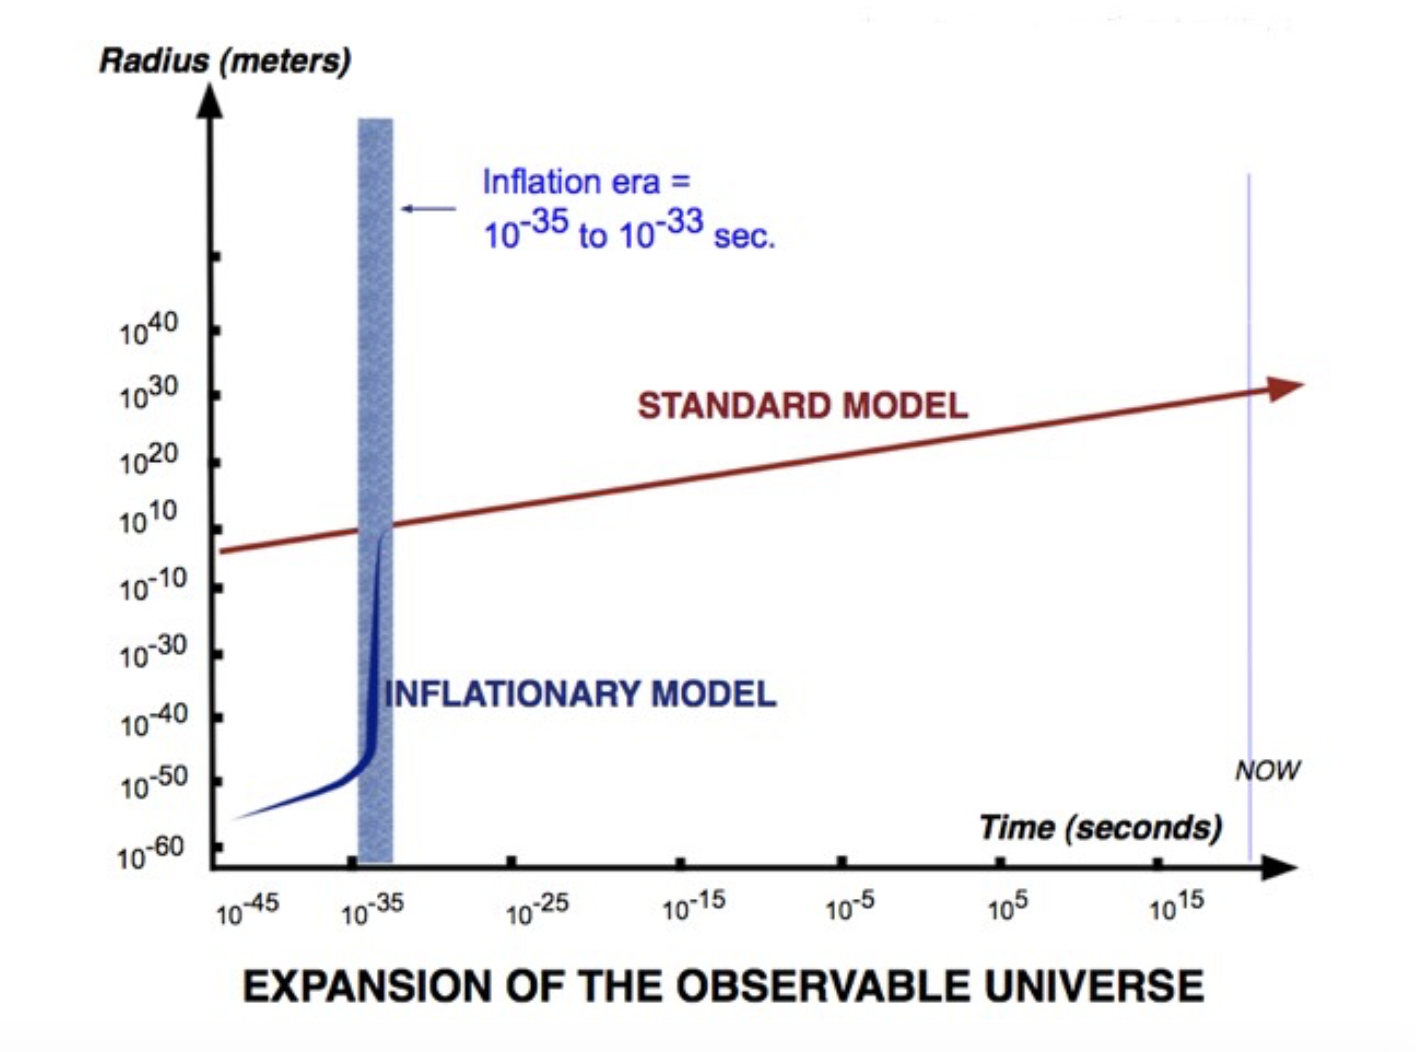
\includegraphics[width=7cm, height=7cm]{images/inflation.png}
    \caption{Modelli a confronto.}
    \label{fig:inflazione}
\end{figure}
\begin{equation}
\mathcal{L}_{\phi}=\frac{1}{2}\dot{\phi}^2-V(\phi,T)
\end{equation}
\begin{equation}
\begin{cases}
\rho_{\phi}=\frac{1}{2}\dot{\phi}^2+V(\phi,T)
\\
P=\frac{1}{2}\dot{\phi}^2-V(\phi,T)
\end{cases}
\end{equation}
Per studiare la transizione di fase \'{e} utile studiare l'equazione di Eulero-Lagrange:
\begin{equation}
\ddot{\phi}+3\frac{\dot{a}}{a}\dot{\phi}+\frac{\partial V}{\partial \phi}=0
\end{equation}
Inoltre l'equazione di Friedmann si modifica tenendo conto anche di $\rho_{\phi}$ che \'{e} anch'esso funzione di $V(\phi,T)$ e sotto l'ipotesi $\rho_{\phi}>>\frac{kc^2}{a^2}$ abbiamo $(\frac{\dot{a}}{a})^2\simeq \frac{8\pi G}{3}\rho_{\phi}$. 
\begin{enumerate}
\item $T>T_c$
\item $T\sim T_c \Rightarrow \dot{\phi} <<V_{\phi}$ "rotolamento lento" $\Rightarrow \rho_{\phi}\sim V_{\phi}\sim k$ inizia la transizione di fase dell'inflatone
\item $T<T_c$ l'inflatone oscilla attorno al suo nuovo equilibrio e si conclude la transizione
\end{enumerate}
\begin{figure}[htp]
    \centering
    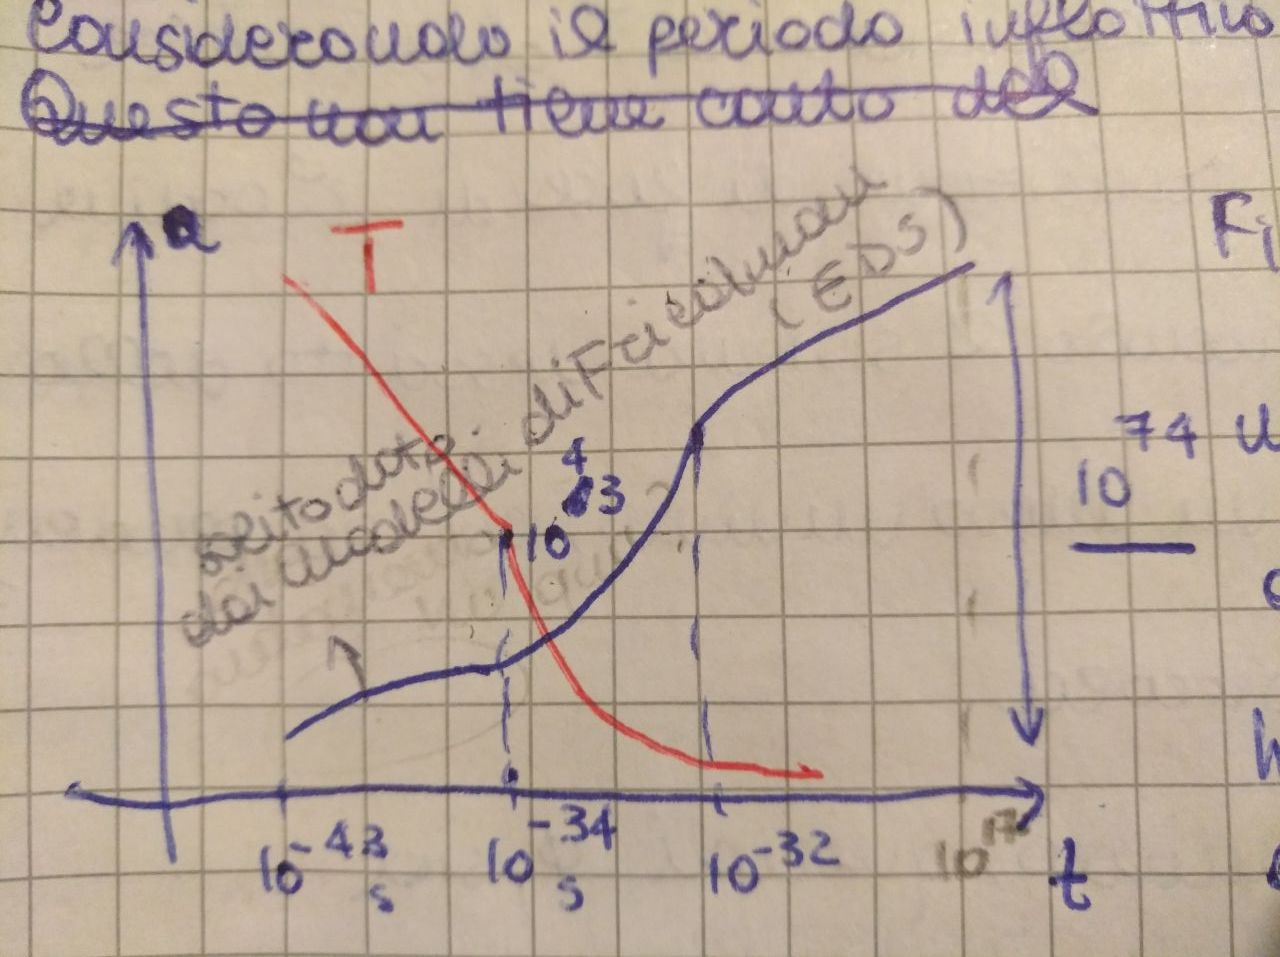
\includegraphics[width=7cm, height=7cm]{images/scala.jpeg}
    \caption{Andamento del fattore di scala.}
    \label{fig:scala}
\end{figure}
\begin{enumerate}
\item $t<10^{-34}$ a segue l'andamento del modello standard del BB
\item $10^{-34}<t<10^{-32}$ si ha un espansione esponenziale, $a(t)\propto \exp{\frac{t}{\tau}}$ con $\tau=10^{-34}$ , l'universo aumenta di 43 ordini di grandezza $\frac{a_f}{a_i}=10^{43}$.
\item $t>10^{-32}$ si conclude la transizione di fase
\end{enumerate}
In conseguenza ad una espansione adiabatica la T dovrebbe diminuire di 43 ordini di grandezza come la $T_{CMB}$, ma cos\'{i} non \'{e} in quanto la transizione di fase rilasci il \textbf{calore latente}\footnote{L'energia del calore latente viene usata per produrre nuove particelle durante tutta la fase del rotolamento lento.} nell'universo, rappresentato dal termine di smorzamento $3\frac{\dot{a}}{a}\dot{\phi}$ , la temperatura risale di 43 ordini di grandezza questo fenomeno prende il nome di \textbf{re-heating}.
\subsection{Risoluzione dei problemi di HBB}
\subsubsection{Risoluzione Monopoli}
Si fa partire l'inflazione dopo la formazione dei monopoli magnetici che vengono prodotti a $t=10^{-35}s$ (con una transizione di fase del periodo di GUT), si ha dunque un solo monopolo per universo visibile che ha probabilit\'{a} trascurabile di essere osservato da terra.
\subsubsection{Risoluzione l'orizzonte}
Prima dell'inflazione le regioni che ora consideriamo separate causalmente erano connesse.
\begin{equation}
\begin{cases}
\rho_{\phi}=k
\\
P=\frac{1}{2}\dot{\phi}^2-V(\phi,T), \quad \phi<< V(\phi)
\end{cases}
\end{equation}
Dalla conservazione del tensore energia impulso ottengo una condizione sugli orizzonti cosmologici $(\frac{a_f}{a_i})^{-3(w+1)}>>\frac{T_f}{T_i}\cdot 10^{59}$ da cui conseguono:
\begin{enumerate}
\item Universo vuoto dominato da una costante cosmologica quindi $w=-1$
\item  $\frac{a_f}{a_i}>>\frac{T_f}{T_i}\cdot 10^{30}$ in cui $T_f$ dipendendo dal \textbf{re-heating}\footnote{Dunque dal modello inflazionario usato ha un possibile fluttuazione.}
\item $\frac{T_f}{T_i}\in [10^{-5}, 1]$ considerando il limite inferiore produce $T_f > 10^{14} GeV$ che \'{e} concorde con un modello di inflazione con $10^{-34}<t<10^{-32}$ che implica $\frac{a_f}{a_i}\sim 10^{43}$
\end{enumerate}
\subsubsection{Risoluzione della Piattezza}
L'universo all'epoca di Planck pu\'{o} avere un valore di $\Omega_0$ arbitrario, ma poi questo verra\'{a} spinto a $\Omega_0=1$ dall'inflazione, indipendentemente dal valore iniziale di questo. Dalla conservazione del tensore E-I otteniamo $\frac{a_f}{a_i}>>(\frac{\Omega_i^{-1}-1}{\Omega_0^{-1}-1})^{\frac{1}{2}}\frac{T_f}{T_i}\cdot 10^{30}$  che per mette a $\Omega_0 \rightarrow 1$.
\subsection{Problema della costante cosmologica}
Il modello standard del Big Bang non riesce a spiegare il problema di \textbf{fine tuning} della costante cosmologica, inserita nei modelli di Friedmann come componente aggiuntiva. Secondo QFT l'universo nasce con una certa energia iniziale $\Lambda$ interpretata come l'energia del livello fondamentale, a cui \'{e} associato il campo scalare $\phi_{\Lambda}$ con il suo potenziale $V(\phi,T)$. Durante le \textbf{transizione di fase} parte di questa energia viene liberata tramite calore specifico, pu\'{o} essere stimata come $\Delta\rho_{V,i}\sim m_i^4$:
\begin{enumerate}
\item GUT: $m\sim10^{15} GeV$
\item SUSY: $m\sim10^{3} GeV$
\item E-W: $m\sim10^{2} GeV$
\item Q-H: $m\sim10^{-1} GeV$
\end{enumerate}
Poich\'{e} l'energia del vuoto si conserva si stima essere $\rho_V(t_P)= \Delta \rho_V+\rho_V(t_0)$ con  $\Delta\rho_V\sim \sum_i \Delta\rho_{V,i} \sim 10^{60} GeV$ somma dell'energia liberata durante le transizioni e la densit\'{a} oggi a cui \'{e} associata la costante cosmologica. Stiamo mettendo insieme QFT e GR, allora $\rho_V(t_0)c^2=\Omega_{\Lambda0}\rho_{c0}c^2$ che troviamo mettendo assieme informazioni sull'espansione dell'universo (SNIa) e la piattezza (CMB):
\begin{itemize}
\item $\Omega_0-\Omega_{\Lambda0}=-0.53$ (SNIa)
\item $\Omega_{\Lambda0}+\Omega_0=1$ (CMB)
\item $\Omega_0=0.3$ (LSS)
\end{itemize}
Da cui $\rho_V(t_0)\simeq10^{-46} GeV^4$ e quindi $\rho_V(t_P)= \Delta \rho_V(1+ 10^{-106})$, quindi la densit\'{a} di energia del livello fondamentale associata al vuoto deve coincidere con la somma della densit\'{a} di energia di tutte le transizioni di fase che sarebbero avvenute successivamente a meno di una parte su $10^{106}$. Quindi o scopriremo una nuova transizione con $\Delta\rho_{V}\sim 10^{-46} GeV^{4}$ oppure resteremo con una costante cosmologica problematica.
\subsection{Risoluzione del problema della costante Cosmologica}
Facciamo un breve escursus sulle identit\'{a} delle costanti in fisica:
\begin{itemize}
\item Costanti di \textbf{accoppiamento}: si determinano sperimentalmente (ex. \textbf{G})
\item Costanti \textbf{additive}: associate a quantit\'{a} di cui mi interessa la differenza (ex. ddp)
\end{itemize}
Mentre la $\Lambda$ \'{e} una costante anomala in quanto non riconducibile a nessuana delle due categorie.
\begin{itemize}
\item GR: assume un ruolo geometrico o di sorgente a seconda di dove compare nell'equazione di E.
\item QFT: assume significato di \textbf{densit\'{a} di energia del vuoto} produce un problema di fine tuning.
\end{itemize}
L'ipotetica soluzione sarebbe quella di associare ad essa un campo scalare  indicato come \textbf{energia oscura} \footnote{A pressione negativa e contenente il $70\%$ della densit\'{a} dell'universo ($\Omega_0+ \Omega_{\Lambda 0}=0.7$).}. Se si dimostrasse che $w=w(z)$, da osservazioni sull'evoluzione temporale delle strutture cosmiche, potremmo dimostrare l'esistenza del campo scalare energia oscura. Ma questo ci riporterebbe ad una visione Aristotelica dell'universo costituito prevalentemente dalla \textbf{quinta essenza}, che non posso vedere\footnote{Modelli di quinta essenza.}.\\ In conclusione ci comportiamo come se l'universo oggi avesse costante cosmologica, che introduciamo ad Hoc in modo da riporre i dati osservativi. Questo approccio ci da informazioni sulla validit\'{a} del modello.
\subsection{Big Bang nucleosynthesis}
Gamow, Alpher and Herman proposed the hot Big Bang as a means to produce all of the elements. However, the lack of stable nuclei with atomic weights of 5 or 8 limited the Big Bang to producing hydrogen and helium. Burbidge, Burbidge, Fowler and Hoyle worked out the nucleosynthesis processes that go on in stars, where the much greater density and longer time scales allow the triple-alpha process (He+He+He = C) to proceed and make the elements heavier than helium. But BBFH could not produce enough helium. Now we know that both processes occur: most helium is produced in the Big Bang but carbon and everything heavier is produced in stars. Most lithium and beryllium is produced by cosmic ray collisions breaking up some of the carbon produced in stars.
\subsection{Stages of the early universe}
The following stages occur during the first few minutes of the Universe:
\begin{itemize}
\item Less than 1 second after the Big Bang, the reactions shown at right maintain the neutron:proton ratio in thermal equilibrium. About 1 second after the Big Bang, the temperature is slightly less than the neutron-proton mass difference, these weak reactions become slower than the expansion rate of the Universe, and the neutron:proton ratio freezes out at about 1:6.
\item After 1 second, the only reaction that appreciably changes the number of neutrons is neutron decay, shown at right. The half-life of the neutron is 615 seconds. Without further reactions to preserve neutrons within stable nuclei, the Universe would be pure hydrogen.
\item The reaction that preserves the neutrons is deuteron formation. The deuteron is the nucleus of deuterium, which is the heavy form of hydrogen (H2). This reaction is exothermic with an energy difference of 2.2 MeV, but since photons are a billion times more numerous than protons, the reaction does not proceed until the temperature of the Universe falls to 1 billion K or kT = 0.1 MeV, about 100 seconds after the Big Bang. At this time, the neutron:proton ratio is about 1:7.
\item Once deuteron formation has occurred, further reactions proceed to make helium nuclei. Both light helium (He3) and normal helium (He4) are made, along with the radioactive form of hydrogen (H3). These reactions can be photoreactions as shown here. Because the helium nucleus is 28 MeV more bound than the deuterons, and the temperature has already fallen so far that kT = 0.1 MeV, these reactions only go one way.
\item The reactions at right also produce helium and usually go faster since they do not involve the relatively slow process of photon emission.
\item The net effect is shown at right. Eventually the temperature gets so low that the electrostatic repulsion of the deuterons causes the reaction to stop. The deuteron:proton ratio when the reactions stop is quite small, and essentially inversely proportional to the total density in protons and neutrons. Almost all the neutrons in the Universe end up in normal helium nuclei. For a neutron:proton ratio of 1:7 at the time of deuteron formation, 25\% of the mass ends up in helium.
\end{itemize}

\subsection{Abundance of light elements depending on the density of baryons}
The deuterium, He3, He4 and Li7 abundances depend on the single parameter of the current density of ordinary matter made out of protons and neutrons: baryonic matter. The graph above shows the predicted abundance vs. baryon density for these light isotopes as curves, the observed abundances as horizontal stripes, and the derived baryon density as the vertical stripe. A single value of the baryon density fits 4 abundances simultaneously. The fit is good but not perfect. There has been a dispute about the actual primordial helium abundance in the Universe: either 23.4 or 24.4 percent by mass, with both broups claiming 0.2 percent accuracy so this is 5 sigma discrepancy between the different observational camps. And a new measurement of the free neutron lifetime is 6 sigma smaller that the previous world average, giving a new prediction of the helium abundance of 24.6 percent. The observed lithium abundance in stars is less than the predicted lithium abundance, by a factor of about 2. But stars destroy lithium so it is hard to assess the significance of this difference. 
\newpage
\section{Formazione di strutture cosmiche}
\subsection{Problemi della formazione di strutture}
L'universo \'{e} omogeneo e isotropo su larga scala ovvero per $L>100Mpc$, mentre non \'{e} cos\'{i} su piccola scala in quanto abbiamo strutture come galassie e ammassi. Definendo il \textbf{contrasto di densit\'{a}} come  $\delta_{stuct}=\frac{\rho_{struct}-\bar{\rho}}{\bar{\rho}}$ con $\bar{\rho}\sim \rho_c$ si ha uno strumento che identifica quanto la struttura in considerazione \'{e} pi\'{u} densa della densit\'{a} critica. Vediamo che quando consideriamo i super ammassi ($R\sim 10Mpc$ e $M\sim 10^{15}-10^{16} M_{\odot}$)  $\delta_{sup}\sim 1-10$. \\Le strutture cosmiche si pensa si siano originate dalle perturbazioni del campo di densit\'{a}, che attraverso l'instabilit\'{a} gravitazionale hanno aggregato materia ed evolvendo nel tempo hanno formato la struttura su larga scala. Due problemi sono:
\begin{enumerate}
\item Condizioni iniziali delle fluttuazioni: il modello inflattivo considera il \textbf{principio di indeterminazione} di Heisenberg come fenomeno alla base delle \textbf{fluttuazioni quantistiche pre-inflattive}
\item Il tempo necessario all'instablitit\'{a} per evolvere\footnote{Se l'et\'{a} dell'universo \'{e} sufficiente per far sviluppare queste strutture?}: devo studiare il campo di velocit\'{a} della materia.
\end{enumerate}
\subsection{Crescita delle perturbazioni in un universo in espansione}
Trattiamo il campo di densit\'{a} come un\textbf{fluido auto-gravitante}, le cui condizioni iniziali sono determinate dal periodo preinflattivo. Le equazioni che lo descrivono sono 4:
\begin{equation}
\begin{cases}
\frac{\partial \rho}{\partial t}+\nabla \textbf{v}=0 
\\
\frac{\partial v}{\partial t}+(\textbf{v}\cdot\nabla)\textbf{v}= -\frac{1}{\rho} \nabla P-\nabla \phi
\\
\nabla^2 \phi=4 \pi G \rho
\\
P=P(\rho)
\end{cases}
\label{eq:autog}
\end{equation}
Le equazioni \ref{eq:autog} \'{e} fornisco un approccio classico al problema, ovvero \'{e} un approccio newtoniano in quanto in limite di campo debole.($a=a_{bkg}+a_1, \quad a_1<<a_{bkg}$) trov\'{o} una soluzione .
\begin{itemize}
\item Per universo \textbf{statico} esistono solo soluzioni triviali a $\rho=0$
\item Per universo in \textbf{espansione} esistono soluzioni a $\rho \neq 0$
\end{itemize}
 Di questo se ne occup\'{o} \textbf{Jeans}, da cui l'instabilit\'{a} gravitazionale prende il nome, il quale facendo uno sviluppo perturbativo al primo ordine dei campi in gioco trov\'{o} l'equazione che regola lo sviluppo temporale delle \textbf{perturbazioni di densit\'{a} $\delta$}in presenza di forze autograv., di pressione e variazione di coordinate proprie in ragione del fattore di scala:
 \begin{equation}
 \ddot{\delta}+2\frac{\dot{a}}{a}\dot{\delta}=\frac{1}{\rho_b a^2}\nabla_x^2P_1+\frac{1}{a^2}\nabla_x^2\phi_1
 \end{equation}
 In coordinate \textbf{proprie} avremo $\dot{\delta}=-\nabla_r \cdot \textbf{v}_1$; mentre in coordinate \textbf{comoventi} $\dot{\delta}=-\nabla_{\textbf{x}}\cdot \textbf{u}$. Inserendo l'equazione di stato nell'ipotesi di \textbf{trasformazione adiabatica} per piccole perturbazioni ($\frac{dP}{d\rho}\sim \frac{P_1}{\rho_1}\sim c_s^2$) ottengo :
 \begin{equation}
 \ddot{\delta}+2\frac{\dot{a}}{a}\dot{\delta}=\frac{c_s^2}{a^2}\nabla_x^2\delta+4\pi G\rho_b \delta
 \end{equation}
 Equazione diff. in $\delta$ spazialmente omogenea, osservo che \'{e} simile all'equazione delle onde. Allora cerco soluzioni della forma di onda piana $\delta\propto \exp{i(\textbf{k}_c\cdot\textbf{x}-\omega t)}$ dove \textbf{x} e \textbf{$k_c$} sono vettori comoventi.
\subsubsection{Instabilit\'{a} di RJ Classica}
La soluzione sar\'{a} una sovrapposizione di onde piane, per un \textbf{fluido statico e omogeneo} da $\textbf{v}_{b}=\dot{a}\textbf{x}$ imponendo staticit\'{a} $\textbf{v}_{bkg}\Rightarrow\dot{a}=0$ ottengo una relazione di dispersione:
\begin{equation}
\omega^2=c_s^2k^2-4\pi G\rho_b
\end{equation}
Con $\textbf{k}_c \cdot \textbf{x}=\textbf{k}\cdot \textbf{r}$. La soluzione varia in funzione di $\omega$:
\begin{itemize}
\item $\omega^2<0 \Rightarrow \delta \propto \exp{-i \omega t}$ (Oscilla a freq. Reale )
\item $\omega^2>0 \Rightarrow \delta \propto \exp{\omega t}$ (Esponenziale a freq. Im.)
\end{itemize}
Definiamo il numero d'onda di Jeans \'{e} $k_J^2=\frac{4\pi G\rho}{c_s^2}$ di conseguenza la \textbf{lunghezza d'onda di Jeans} $\lambda_J=\frac{2\pi}{k_J}=c_s(\frac{\pi}{G\rho_b})^{\frac{1}{2}}$ ci permette di esprimere $\Gamma=\pm \omega=\pm \left\{ 4\pi G\rho_b(1-\frac{\lambda_J}{\lambda})^2\right\}^{\frac{1}{2}}$ inverso del tempo scala del processo $\tau\propto (G \rho_b)^{-\frac{1}{2}}$:
\begin{itemize}
\item $\lambda<\lambda_J$ ($\Gamma \in \Re$): la perturbazione si \textbf{disperde} con un tempo scala $\tau$ in maniera esponenziale ($\exp{-\frac{t}{\tau}}$), i campi di velocit\'{a} sono spostati verso l'esterno.
\item $\lambda > \lambda_J$ ($\Gamma \in \Im$): la perturbazione fa \textbf{collassare} il sistema i cui campi di velocit\'{a} sono diretti verso il centro.
\end{itemize}
\subsubsection{Instabilit\'{a} di RJ in un mezzo in espansione}
\begin{equation}
\ddot{\delta}+2\frac{\dot{a}}{a}\dot{\delta}=-\omega^2 \delta
\label{eq:rjexp}
\end{equation}
Equazione di RJ classica. Impongo:
\begin{itemize}
\item Univ. polvere : $c_s^2k^2<<4\pi G\rho_b$
\item EdS: $\frac{\dot{a}}{a}=\frac{2}{3t}, \quad 4\pi G\rho_b=\frac{2}{3t^2}$
\end{itemize}
\begin{equation}
\ddot{\delta}+\frac{4}{3t}\dot{\delta}+ \frac{2}{3t^2}\delta=0
\end{equation}
La soluzione \'{e} del tipo $\delta \propto t^n$, sostituendo otteniamo l'equazione secolare che mi da i valori di $n=\frac{2}{3}, -1$, di cui ci interessa la soluzione crescente in quanto un EdS $\delta_+\propto a\propto (1+z)^{-1}$ qui la crescita della perturbazione \'{e} algebrica e non esponenziale come nella RJ classica. Per avere piccole perturbazioni si deve considerare un grande z, ci si aspetterebbe che le anisotropie della S\footnote{Brillanza superficiale.} del CMB siano comparabili con il contrasto di densit\'{a}  dei super ammassi in quanto risalenti allo stesso z circa. 
\begin{itemize}
\item $\delta_{SA}(z\sim 1000)\sim 10^{-3}$
\item $\delta_{CMB}\sim 10^{-5}$
\end{itemize}
I dati osservativi differiscono di alcuni ordini di grandezza. Se partiamo dalle anisotropie della CMB le faccio evolvere a $z\sim 1000$ troverei $\delta_{SA} \sim 10^{-2}$ che \'{e} pi\'{u} grande di 	quello che calcolo, ho due ipotetiche soluzioni:
\begin{itemize}
\item le perturbazioni di densit\'{a} si sono evolute pi\'{u} \textbf{rapidamente} di quello che calcoliamo
\item Oppure le perturbazioni del CMB \textbf{non sono connesse} con quelle della materia
\end{itemize}
Introducendo un ulteriore ipotesi, $\Omega_0=0\Rightarrow \rho_b=0$ (\textbf{Universo di Milne}) si ha:
\begin{equation}
\ddot{\delta}+\frac{4}{3t}\dot{\delta}=0
\end{equation}
La soluzione crescente $\delta_+\propto k$ \'{e} consistente, in quanto non essendoci materia la perturbazione non cresce; la soluzione negativa $\delta_- \propto t^{-1}$ fa disperdere la perturbazione .
\begin{figure}[htp]
    \centering
    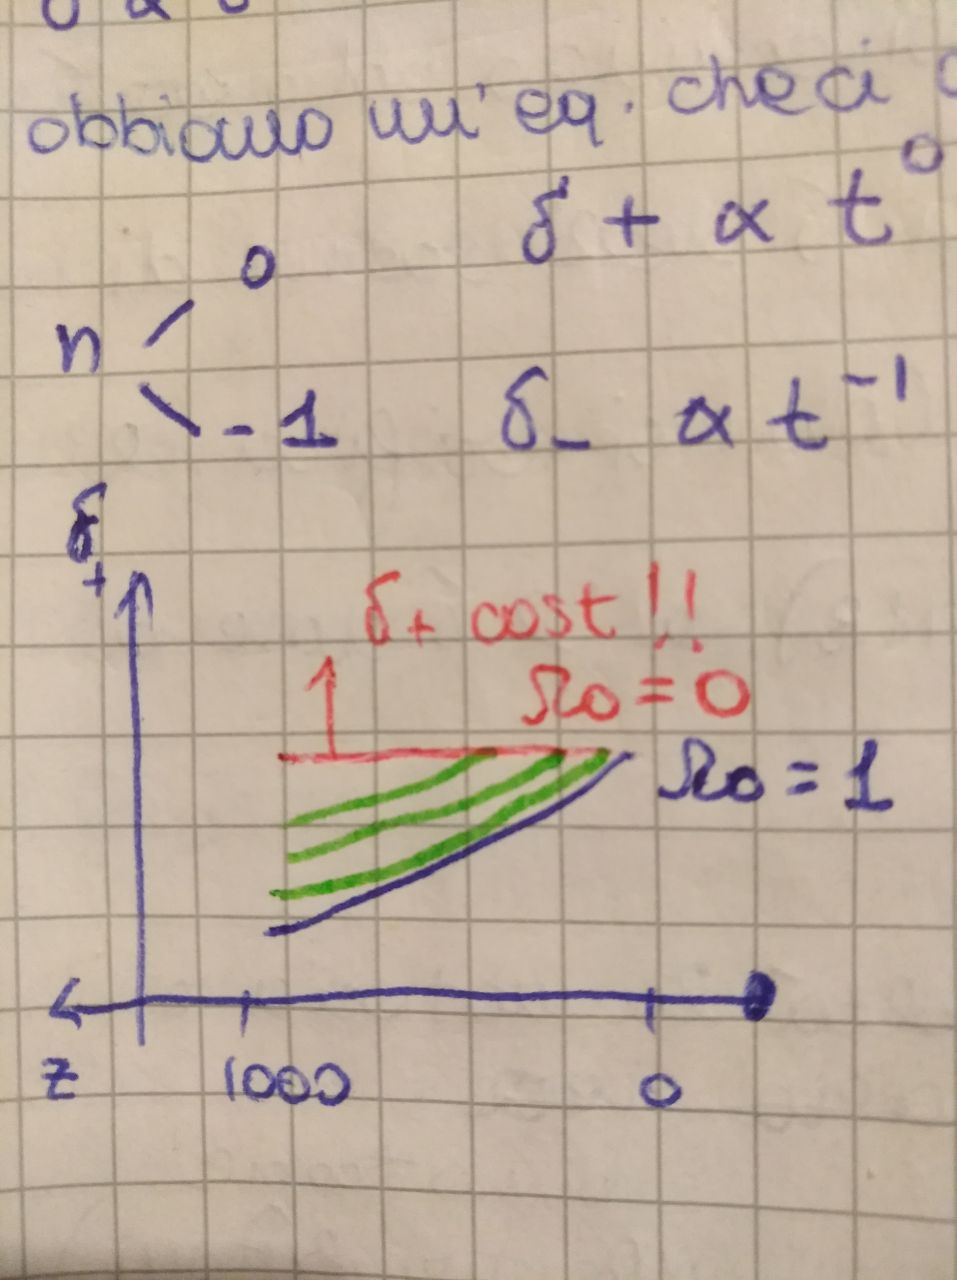
\includegraphics[width=7cm, height=7cm]{images/milne.jpeg}
    \caption{RJ in universo in espansione.}
    \label{fig:milne}
\end{figure}
In definitiva le anisotropie del CMB sono connesse con le perturbazioni di densit\'{a} della materia ordinaria dal disaccoppiamento. Tuttavia la materia oscura costituisce $80\%$ della materia  dell'universo e dunque domina gravitazionalmente sulla materia ordinaria, le sue perturbazioni della densit\'{a} sono $\delta_{DM}\sim 10^{-3}$ non sono connesse alle anisotrie del CMB, in quanto disaccoppiate. La GR e l'instabilit\'{a} di Jeans sono valide e spiegano la formazione di strutture cosmiche a patto che  esista una nuova forma di materia non barionica. La formazione di strutture cosmiche e l'abbondanza di elementi leggeri implicano la presenza di DM indipendentemente.
\subsubsection{Soluzione generale per instabilit\'{a} di RJ}
Patendo dall'equazione \ref{eq:rjexp} e risolvendola nel caso pi\'{u} generale possibile:
\begin{itemize}
\item $0<\Omega<1$
\item $w=0$ (Polvere)
\item $c_s^2k^2<<4\pi G\rho_b$ con $\rho_{b}\propto a^{-3}$
\end{itemize}
\begin{equation}
\delta_+=\frac{5}{2} \Omega_0 \frac{\dot{a}}{a}\int_0^a \frac{da'}{(\dot{a'})^3}=D(a)
\end{equation}
Si def. $D(a)$ \textbf{fattore di crescita} \footnote{Come crescono le perturbazioni in teoria lineare.}. Questo integrale \'{e} analogo a quello che ho trovato nel caso della risoluzione all'eq. di Friedmann:
\begin{equation}
\begin{cases}
t=\frac{\Omega_0}{2H_0(1-\Omega_0)^{\frac{3}{2}}}(\sinh{\theta}-\theta)
\\
a=\frac{\Omega_0}{2(1-\Omega_0)}(\cosh{\theta}-1)
\end{cases}
\end{equation}
Il fattore di scala in un universo in espansione cresce con una potenza del tempo e non in maniera esponenziale, dipende da $\Omega(a)$ e $\Omega_{\Lambda }(a)$;  questo \'{e} normalizzato all'universo di EdS in quanto  $D(a)=1$.
\begin{equation}
D(a)=\frac{\frac{5}{2}\Omega(a)}{\Omega^{\frac{4}{7}}- \Omega_{\Lambda}(a)+(1+\frac{\Omega(a)}{2})(1+\frac{\Omega_{\Lambda}(a)}{2})}
\end{equation}
Un'altra funzione per il fattore di crescita \'{e}:
\begin{equation}
f(a)=\frac{d\ln{D(a)}}{d\ln(a)}\simeq \Omega(a)^{0.6}+\frac{\Omega_{\Lambda 0}(a)}{70}\left\{1+\frac{\Omega(a)}{2}\right\}
\end{equation}
Si nota che il termine $\Omega_{\Lambda}$ non \'{e} da trascurare in quanto ha un ruolo nella formazione di strutture: se $\Lambda>0$ allora  \'{e} un termine \textbf{repulsivo} (negativo), che va aggiungersi al fattore di \textbf{attrito di Hubble}, questo comporta che le strutture cosmiche tendano a \textbf{congelarsi} prima rispetto ad un universo con $\Lambda<0$.
\begin{figure}[htp]
    \centering
    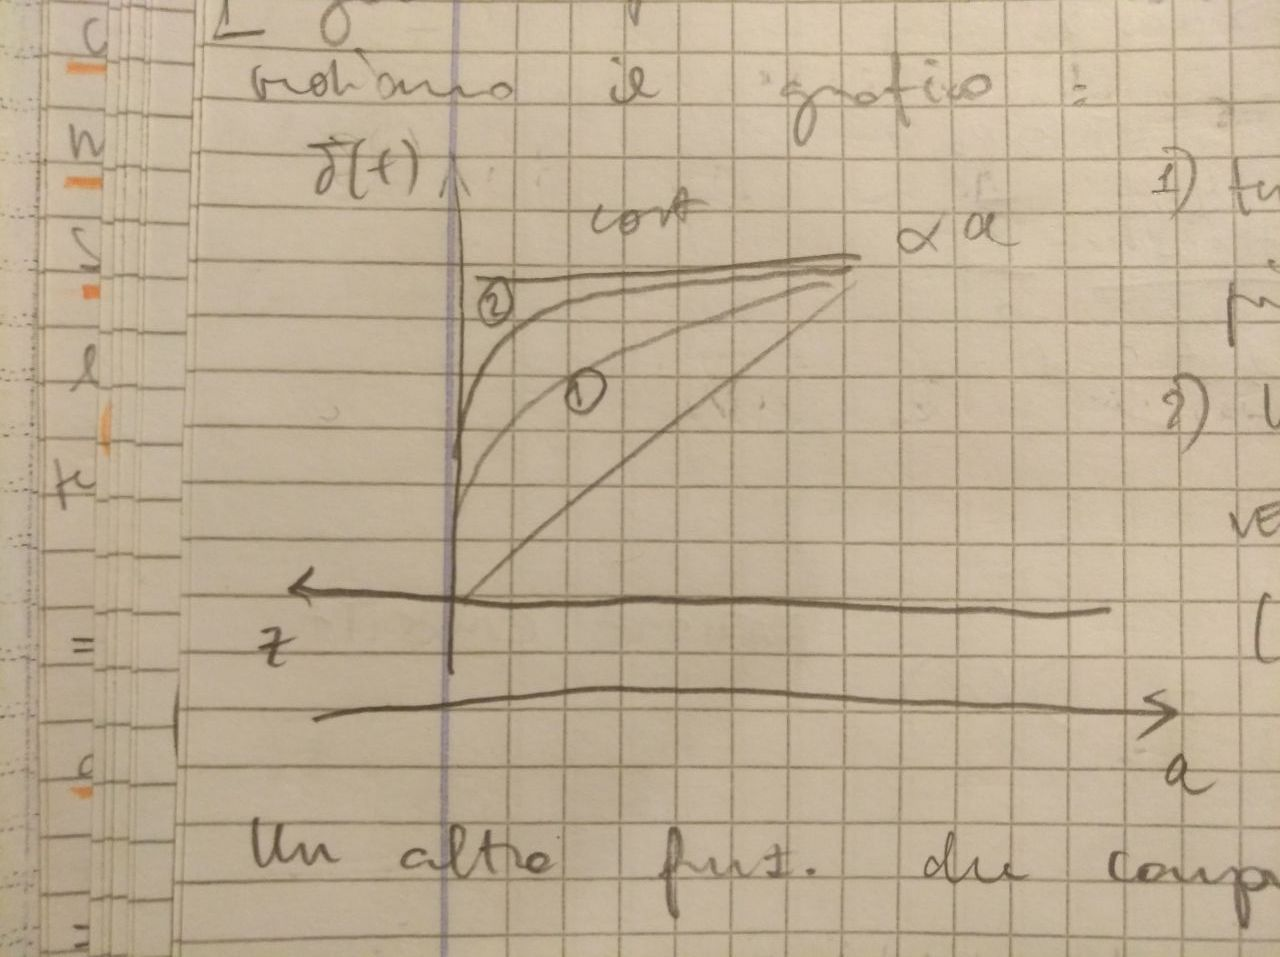
\includegraphics[width=7cm, height=7cm]{images/pertgen.jpeg}
    \caption{Perturbazioni di densit\'{a}.}
    \label{fig:pertgen}
\end{figure}
\begin{enumerate}
\item Le perturbazioni da piccole crescono progressivamente fino a congelarsi
\item In un universo con $\Lambda\neq0$ succede la stessa cosa ma pi\'{u} rapidamente
\end{enumerate}
Osserviamo che  $\Omega_{\Lambda }(a)$ \'{e} trascurabile rispetto a $\Omega(a)$ 
\subsubsection{Fluido relativistico}
Studiamo l'evoluzione delle perturbazioni di densit\'{a} per un fluido relativistico. Si aggiunge una sorgente di energia legata alla $P=\frac{1}{3}\rho c^2$, dunque sostituiamo $\rho \rightarrow \rho +\frac{3P}{c^2}$ . Siccome l'equazione cambia abbiamo che $\lambda_J=c_s (\frac{3\pi}{8G\rho_b})^{\frac{1}{2}}$ che porta ad uno sviluppo delle perturbazioni differente.
Se $z\rightarrow \infty$ allora $\Omega \sim 0$ siamo in EdS\footnote{L'universo primordiale, dominato da radiazione, \'{e} ben approssimabile da EdS.} con $\delta_+\propto t$ e $\delta_- \propto t^{-1}$ :
\begin{itemize}
\item $t<t_{eq}$ (U. di radiaz.): $a\propto t^{\frac{1}{2}}\Rightarrow \delta_+\propto a^2$ 
\item $t>t_{eq}$ (U. di polvere): $a\propto t^{\frac{2}{3}}\Rightarrow \delta_+\propto a$ 
\end{itemize}
\subsubsection{Evoluzione delle velocit\'{a} peculiari}
Le perturbazioni del campo di densit\'{a} sono accoppiate al campo di velocit\'{a}. Considerando l'equazione di Eulero con incognita la velocit\'{a} comovente (in U. polvere) posso dividerla in componenti rispetto al potenziale.
\textbf{Moti Rotazionali}: $\dot{\textbf{u}}_{\perp}+2\frac{\dot{a}}{a}\textbf{u}_{\perp}=0 \Rightarrow u _{\perp}\propto a^{-2}$ quindi $v_{1\perp}= a u _{\perp}\propto a^{-1}$ 
Le componenti rotazionali delle perturbazioni di densit\'{a} vengono spazzate via a causa dello \textbf{smorzamento} che subisce la componente rotazionale del campo di velocit\'{a} con l'espansione dell'universo. Le strutture cosmiche hanno per\'{o} un momento angolare che non \'{e} legato alle condizioni iniziali della velocit\'{a}, bens\'{i} generato dalle interazioni mareali durante l'evoluzione delle strutture stesse. Gli effetti del momento angolare iniziale \'{e} trascurabile in teoria lineare.
\textbf{Moti Potenziali}: $\dot{\textbf{u}}_{\parallel}+2\frac{\dot{a}}{a}\textbf{u}_{\parallel}=-\frac{1}{a^2}\nabla\phi_1$. Sviluppo in onde piane:
\begin{equation}
\begin{cases}
\phi_1 \propto \exp{i(k_cx-\omega t)}
\\
u_1 \parallel \nabla\phi_1 \propto i k_c \exp{i(k_cx-\omega t)}
\end{cases}
\end{equation}
Considerando EdSin U. di polvere, sappiamo che $\delta\propto t^{\frac{2}{3}}$ dunque $v_{1\parallel} =\frac{\dot{\delta}}{k_c} \propto \frac{t^{\frac{1}{3}}}{k_c}=\frac{a^{\frac{1}{2}}}{k_c}$.\\
\underline{Pert. Densit\'{a}}: cresce qualora la perturbaxzione \'{e} sovradensa.\\
\underline{Campo di Velocit\'{a}}: le velocit\'{a} peculiari ($v_{1\parallel}\propto \frac{1}{k_c}$) non possono essere studiate localmente in quanto ho contributi derivanti dalle perturbazioni di densit\'{a} su larga scala. Le velocit\'{a} peculiari dipendono dalla scala spaziale delle perturbazioni che le generano ($\lambda_c=\frac{2\pi}{k_c}$).\\ 
Se vogliamo giustificare la formazione di strutture cosmiche per instabilit\'{a} gravitazionale nel framework della GR troviamo che l'evoluzione di queste in un universo in espansione \'{e} lenta rispetto ad un universo statico.
\subsubsection{Stima della densit\'{a} della velocit\'{a} peculiare}
\underline{Metodo 1:}
\begin{equation}
\begin{cases}
\left|v_{1\parallel}\right|=\frac{a\dot{\delta}}{k_c}
\\
\delta(a, \textbf{x})=D(a) \delta_i(\textbf{x})
\\
f(a)\simeq \Omega^{0.6}
\end{cases}
\end{equation}
Da cui facendo le dovute sostituzioni, e considerando larga scala ($k_c\sim r$ ), ottengo la velocit\'{a} propria che coincide con la velocit\'{a} peculiare comovente $\left|v_{1\parallel}(t_0)\right|=r H_0\Omega_0^{0.6}\delta_0$. Ipotizzando che la massa \'{e} tutta contenuta nelle galassie $\delta$ lo stimo dalle galassie essere $\delta_g\simeq
b\delta$ dove il bias \'{e} $b=b(t,z)$ che indica il rapporto tra il contrasto di densit\'{a} in galssie e quello totale.
\begin{equation}
\left|v_{1\parallel}(t_0)\right|=r H_0\frac{\Omega_0^{0.6}}{b}\delta_{g0}
\end{equation}
\begin{itemize}
\item $\delta_{g0}$ lo misuro dalla distrib. di materia nello spazio
\item $v_{1\parallel}(t_0) \equiv v_{pec}$ allora da Hubble  $v_{1\parallel}(t_0)=cz- H_0 d$ dalla TF e $D_n -\sigma_0$ prendo d
\item b dalle anisotropie del CMB 
\end{itemize}
Ho un errore anche del 100\%.\\
\underline{Metodo 2:}
\begin{equation}
\begin{cases}
\dot{\delta}=-\nabla_r\textbf{v}_1
\\
\dot{\delta}=-\delta f(a)H(a)
\end{cases}
\end{equation}
Ricavo $\delta$ la inserisco nell'equazione di Poisson da cui esplicitando la velocit\'{a} si ha $\textbf{v}_{1\parallel}=-\frac{2}{3}f(a)\frac{\nabla_r \phi_1}{H(a)\Omega(a)}$  e infine $\Omega^{-1}=\frac{3H^2}{8\pi G\rho_b}$.
\subsubsection{Evoluzione delle perturbazioni di densit\'{a} adiabatiche}
Consideriamo la visione semplificata che i cosmologi avevano negli anni 70 in cui le galassie si formano per evoluzione delle perturbazioni di densit\'{a} di materia ordinaria e vanno a sormare i Super Ammassi, le strutture pi\'{u} grandi conosciute al tempo. Studio l'evoluzione delle perturbazioni di densit\'{a} \textit{adiabatiche} (quelle che ho visto fino ad ora) in un universo in espansione costituito da materia ordianaria.\\
\textbf{Scale di spazio}: abbiamo \textit{l'orizzonte cosmologico} $r_H$ (tutto ci\'{o} che \'{e} dentro ha avuto tempo di comunicare con la coordinata in cui mi trovo) ; \textit{scala di perturbazione} $\lambda_J$. La perturbazione evolve se $\lambda<r_H \bigwedge \lambda>\lambda_J$ .\\
\textbf{Scale di massa}: $M_J\propto \rho_B \lambda_J^3$ e $M_H\propto \rho_B r_H^3$. \\
\begin{figure}[htp]
    \centering
    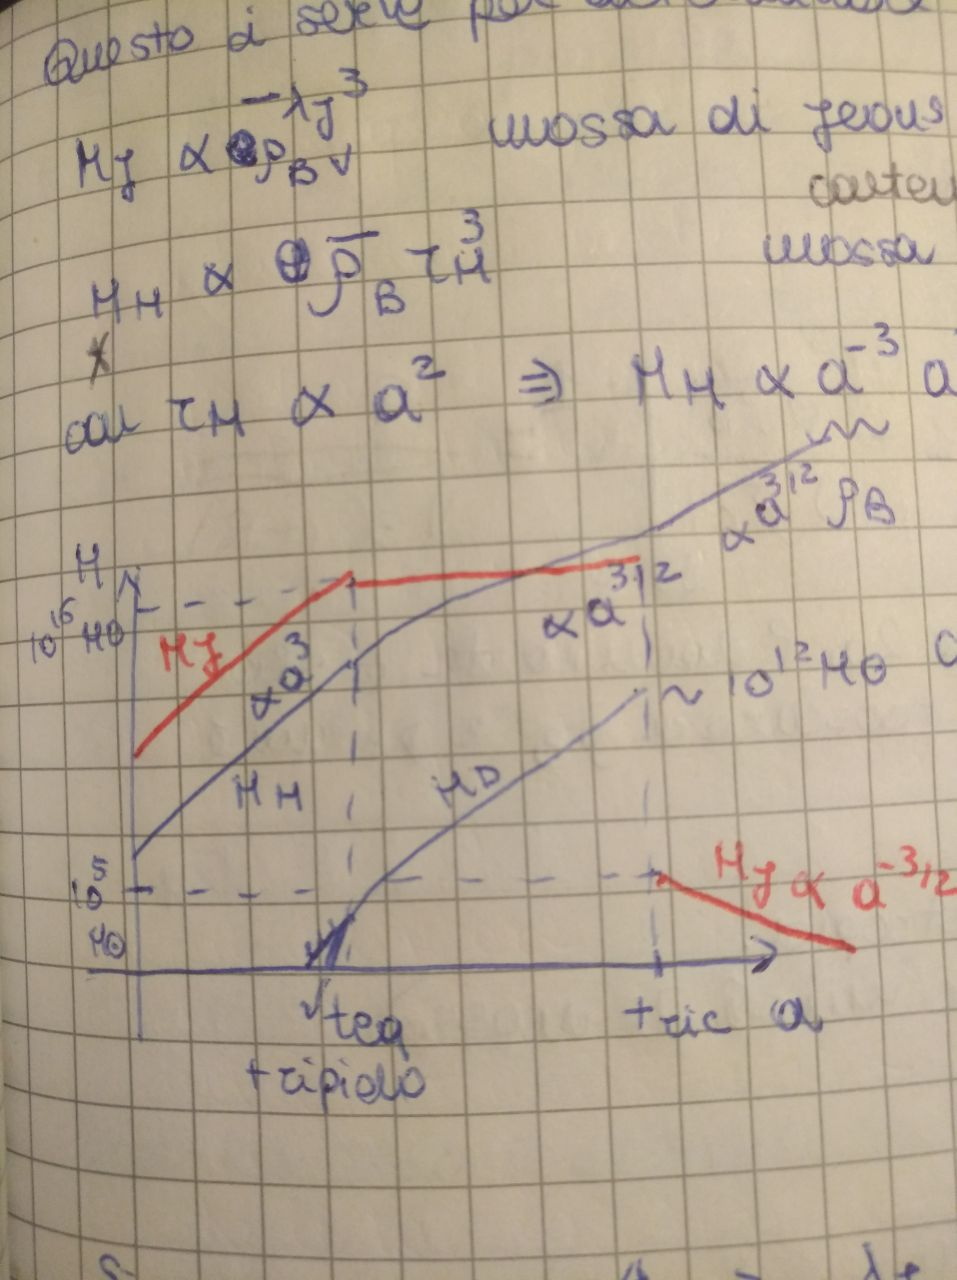
\includegraphics[width=7cm, height=9cm]{images/massev.jpeg}
    \caption{Evoluzione masse (Diaferio).}
    \label{fig:massev1}
\end{figure}
\underline{$t<t_{eq}$} (U. radiazione): \\
\begin{itemize}
\item $r_H\propto a^2 $ e $ \lambda_J\propto a^2$
\item $\rho_{rad}\propto a^{-4}$ e $\rho_B\propto a^{-3}$
\item $M_J\propto a^{3}$ e $M_H\propto a^{3}$
\end{itemize}
Il rapporto $\frac{M_J}{M_H}\simeq 26$ ci dice che $M_J$ sovrasta $M_H$ per\'{o} hanno la stessa dipendenza da $a$.  Le perturbazioni che hanno $\lambda>r_H$, poich\'{e} $M_J>M_H$, crescono con $\delta\propto t$. Queste sono fuori dall'orizzonte cosmologico, quindi dovrei trattarle usando la GR, ma all'ordine zero possiamo pensare che queste siano \textbf{congelate} alle condizioni iniziali. 
\underline{$t_{eq}<t<t_{ric}$} (U. materia): \\
\begin{itemize}
\item $M_J\propto 10^{16} M_\odot\ $ e $ M_H\propto a^{\frac{3}{2}}$
\end{itemize}
Le perturbazioni entrano nell'orizzonte cosmologico nella fase "matter dominant". La $M_J\sim 10^{15} M_\odot\ $ \'{e} costante poich\'{e} \'{e} proporzionale alla densit\'{a} di radiazione e a qualla di materia in una certa potenza tale che si bilancino (funzione di $c_s$ che dipende da $\rho$ ). Le perturbazioni a $M<M_J$ sono in eq. stabile, in oscillano tra collasso grav. e $P_{rad}$, diventano onde sonore che nel tempo si smorzano a causa della perdita di energia adiabatica nell'esp. dell'U.; mentre le pert. con $M>M_J$ continuano a crescere con $\delta\propto a$.\\
\underline{$t>t_{ric}$}: \\
\begin{itemize}
\item $M_J \propto a^{-\frac{3}{2}}$
\end{itemize}
Dopo la ricombinazione $M_J$ decresce col fattore di scala. Quando viene a mancare la $P_{rad}$ (che manteneva $M_J $costante) a causa del disaccoppiamento (che supongo essere istantaneo) $M_J=10^{5} M_\odot\ $, successivamente continua a decrescere come potenza di a. Quindi in questa fase le perturbazioni che prima erano stabili diventa instabili, le perturbazioni che possono collassare diventan $10^5 M_\odot\ $ pi\'{u} grandi.
\begin{figure}[htp]
\centering
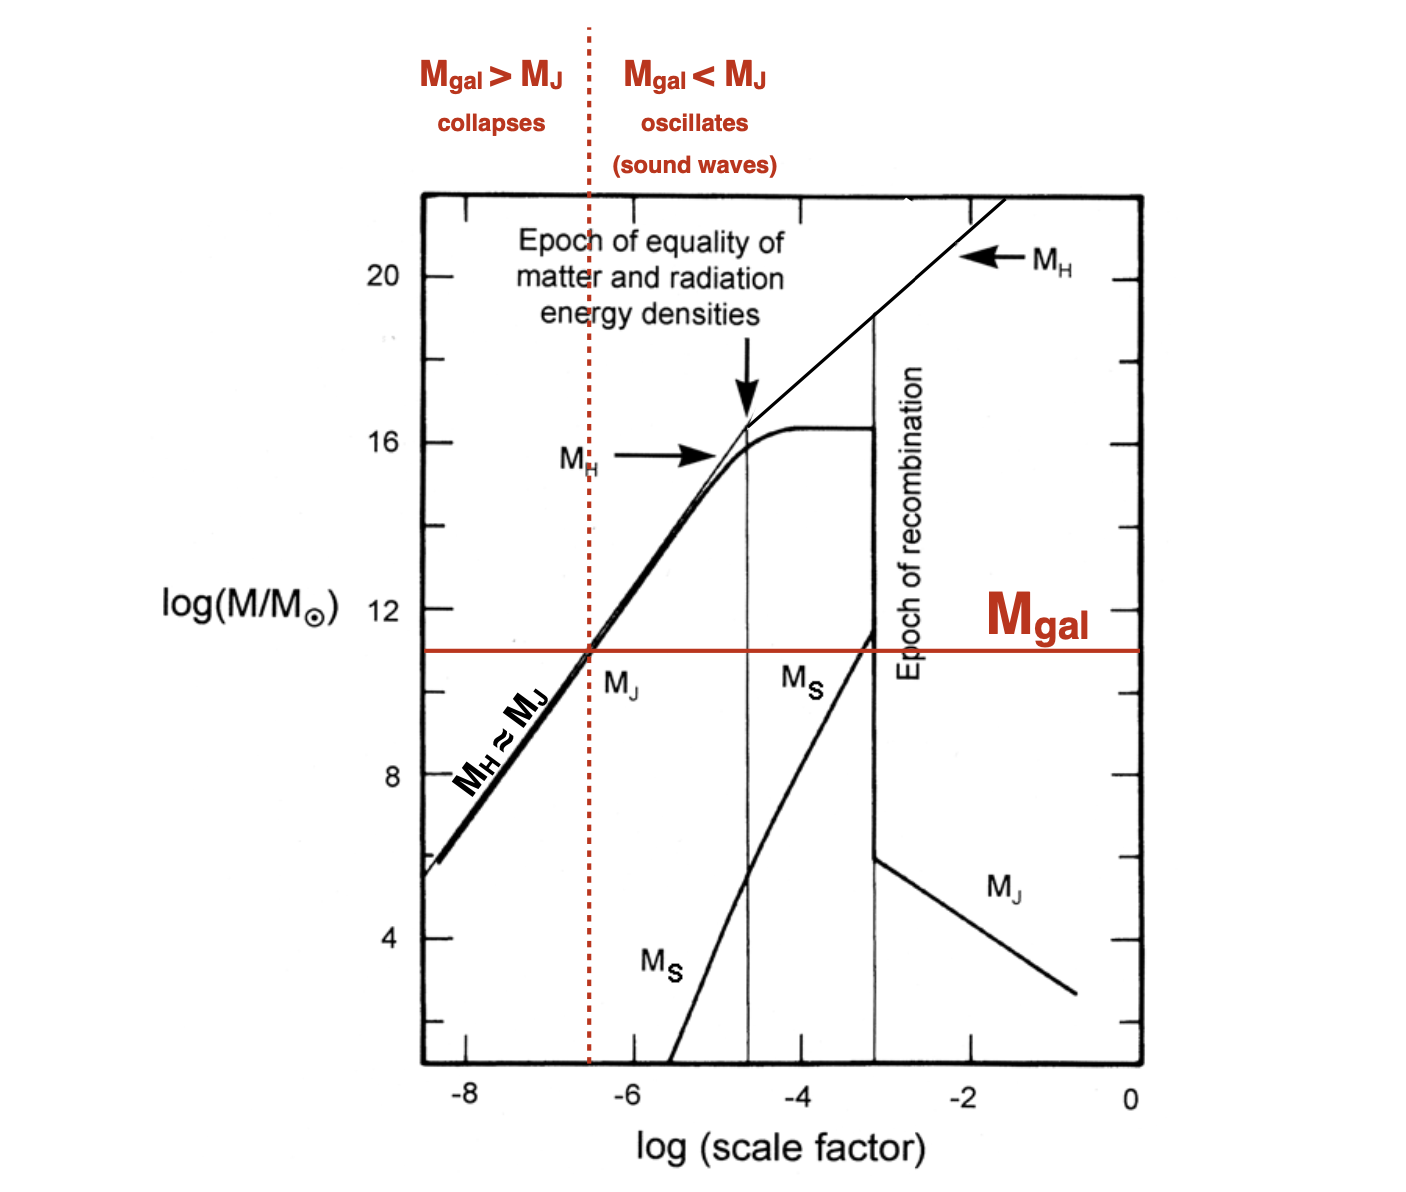
\includegraphics[width=8cm, height=9cm]{images/massev.png}
\caption{Evoluzione della massa di Jeans $M_J$, della massa racchiusa entro l’orizzonte $M_H$ e della massa di Silk $M_S$ in funzione del fattore di scala $a$. La massa di una perturbazione “galattica”, dell’ordine di $10^{11}M_\odot\ $  \'{e} rappresentata da una retta orizzontale in quel diagramma. La riga verticale tratteggiata separa il caso in cui la perturbazione collassa ($M_{gal}>M_J$ ) o oscilla generando onde sonore ($M_{gal <M_J}$ ). Si noti come le scale non corrispondano esattamente ai valori citati nel testo per cui la figura \'{e} da considerarsi come uno schema qualitativo.}
    \label{fig:massev}
\end{figure}
\subsubsection{Processi dissipativi nell'epoca pre-ricombinazione: Silk damping delle perturbazioni adiabatiche}
Per concludere l'evoluzione delle perturbazioni adiabatiche dobbiamo considerare i processi dissipativi che avvengono nell’epoca pre-ricombinazione. Se $\delta$ \'{e} su scale $\lambda<\lambda_J=2 R_H$ allora siamo in presenza di onde sonore adiabatiche dove la forza di richiamo per ogni oscillazione \'{e} data dalla pressione di radiazione; se i fotoni diffondono fuori dalla perturbazione $\delta$ allora le oscillazioni vengono smorzate poich\'{e} viene a mancare la forza di richiamo. Questo fenomeno di smorzamento prende il nome di “\textbf{Silk Damping}”. Considerando la teoria cinetica si ottiene che la lunghezza di “diffusione” dei fotoni al tempo t cio\'{e} il raggio massimo della perturbazione da cui sono in grado di uscire $r_D\propto \sqrt{lct}$ ha una massa di \textbf{Silk} $M_D\propto r_D^3\bar{\rho}_B= a^{\frac{3}{2}} t^{\frac{3}{2}}$ da valutare nell’epoca pre-ricombinazione:
\begin{equation}
\begin{cases}
t<t_{eq} \quad M_D\propto a^{\frac{9}{2}}
\\
t>t_{eq} \quad M_D \propto a^{\frac{15}{4}}
\end{cases}
\end{equation}
La massa di Silk rappresenta la massa massima delle perturbazioni che vengono smorzate a seguito del processo di dffusione dei fotoni;  lo smorzamento interessa tutte perturbazioni “stabili” ovvero che oscillano come onde sonore visto che si ha sempre $M_D<M_J$ . (Dal momento in cui la massa della perturbazione diventa $M_{gal} < M_D$ la perturbazione viene smorzata e la sua ampiezza va rapidamente a 0.)\\
Nel momento della ricombinazione il valore di $M_J\sim 10^{16} M_\odot\ $ crolla istantaneamente \footnote{Se consideriamo ricombinazione istantanea.} a $M_J\sim10^{5} M_\odot\ $ continuando poi a decrescere con $ \propto a^{-\frac{3}{2}}$. Dopo la ricombinazione $M_D\sim 10^{12} M_\odot\ $ , Questo implica che tutte le perturbazioni di tutte le masse, tranne quelle delle galassie piu` massicce, sono state smorzate all'epoca della ricombinazione. Solo le perturbazioni su scale $M>M_{D,rec}$ sopravvivono dopo la ricombinazione. Le strutture su scale pi\'{u} piccole devono essersi necessariamente formate per frammentazione di queste grandi perturbazioni dopo la ricombinazione.
Nel momento della ricombinazione il valore di $M_J\sim 10^{16} M_\odot\ $ crolla istantaneamente \footnote{Se consideriamo ricombinazione istantanea.} a $M_J\sim10^{5} M_\odot\ $ continuando poi a decrescere con $ \propto a^{-\frac{3}{2}}$.
\subsubsection{Evoluzione delle perturbazioni adiabatiche in un universo di DM}
Consideriamo un fluido di materia oscura non collisionale a $t_{infl}<t<t_{eq}$, in quanto le perturbazioni di materia oscura si disaccoppiano prima di quelle di materia ordinaria. In questo caso abbiamo \textbf{smorzamento di Landau}, le velocit\'{a} peculiari relativistiche\footnote{Rispetto ad un sistema di riferimento comovente, si comportano come un fluido di fotoni.} delle particelle sono tali da vincere la velocit\'{a} di fuga dalla buca di potenziale ($v_{pec}>v_{fuga}$), dunque a certe scale (\textbf{free streaming}) la perturbazione viene spazzata via.\\
\begin{equation}
\begin{cases}
r_{fs}= \int_0^{t_{nr}}\frac{v(t)}{a(t)} dt+\int_{t_{nr}}^{t_{eq}}\frac{v(t)}{a(t)} dt
\\
M_{fs}\propto r_{fs}^3 \bar{\rho_{\nu}}
\end{cases}
\end{equation}
Stiamo considerando i neutrini come DM. Spezzo l'integrale in quanto abbiamo un periodo il periodo in cui sono relativistici e quello in cui sono non relativistici. Sotituendo $v\propto t^{-\frac{1}{2}}$ e $a\propto t^{\frac{1}{2}} $ approssimando $t_{eq}\sim t_{nr}$ ottengo $M_{fs}\sim 10^{14} - 10^{15} M_\odot\ $. La materia oscura, sotto queste ipotesi, domina l'evoluzione delle pert. di densit\'{a}. Tutte le perturbazioni a $M<M_{fs}$ vengono smorzate (spazzate via) appena queste entrano nell'orizzonte, la distribuzione di materia \'{e} sostanzialmente omogenea.\\
In questo scenario le strutture si formano per \underline{frammentazione} di perturbazioni pi\'{u} grandi \textbf{Top-Down}. Le osservazioni sono per\'{o} in accordo con uno scenario \textbf{Bottom-Up} in cui le strutture si formano per \underline{aggregazione} di perturbazioni. In sostanza i neutrini non sono la componente dominte della DM, in quanto non influenzano la dinamica delle strutture a larga scala \footnote{Infatti produrrebbero delle strutture diverse da quello che noi conosciamo dalle osservazioni.}. Siccome $m_{\nu}\neq 0 $ questi comunque costituiscono la DM, poniamo un limite alla massa del neutrino $\Omega_{\nu}<\Omega_{lim}$.
\subsubsection{Fluttuazioni barioniche in presenza di DM}
Immaginiamo di avere due fluidi, uno per la materia ordinaria \textbf{barionica} ed uno per la \textbf{materia oscura}. L'evoluzione delle perturbazioni dei due fluidi sar\'{a} descritta da $\ddot{\delta}_i+2\frac{\dot{a}}{a}\dot{\delta}_i=4\pi G \rho_i \delta_i+4\pi G \rho_j\delta_j$, in cui a sinistra troviamo i termini si sorgente del campo gravitazionale. Dal momento per\'{o} che la materia oscura \'{e} dominante rispetto a quella barionica ($\rho_D>>\rho_B$) il nostro sistema di equazioni \textbf{accoppiate} diventa:
\begin{equation}
\begin{cases}
\ddot{\delta}_B+2\frac{\dot{a}}{a}\dot{\delta}_B=4\pi G \rho_D\delta_D
\\
\ddot{\delta}_D+2\frac{\dot{a}}{a}\dot{\delta}_D=4\pi G \rho_D\delta_D
\end{cases}
\end{equation}
Della seconda equaz. abbiamo gia\'{a} la soluzione. Concentriamoci sulla primaipotizziamo EdS ($\Omega_0=1, \quad \rho_D=\rho_C=\frac{3H^2}{8\pi G}$):
\begin{equation}
\begin{cases}
\delta_D\propto a
\\
a\propto t^{\frac{2}{3}}
\end{cases}
\end{equation}
quindi la soluzione \'{e} $\delta_B= B(a-a_1)$. 
\begin{figure}[htp]
\centering
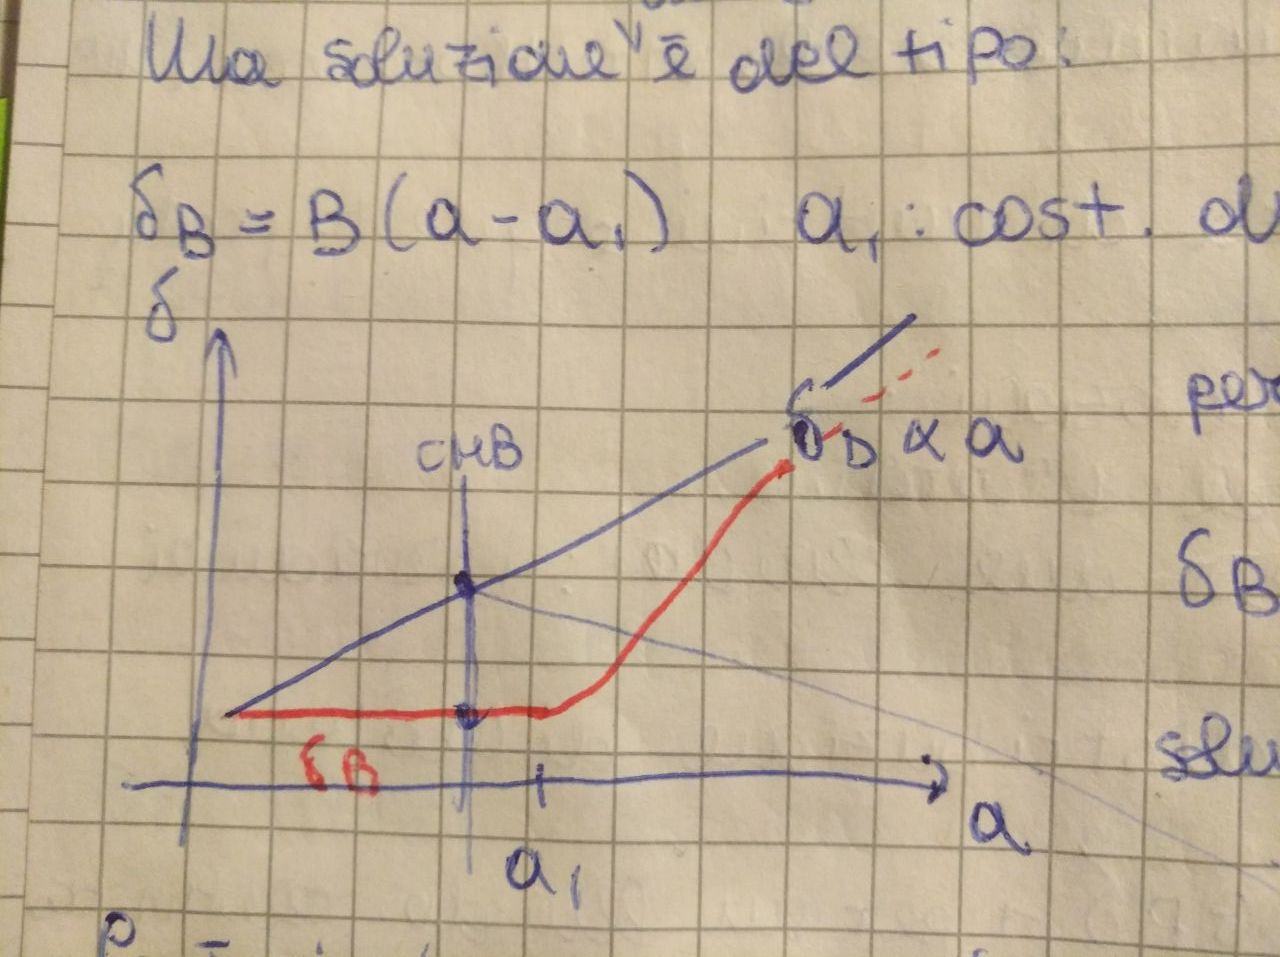
\includegraphics[width=7cm, height=9cm]{images/pertosc.jpeg}
\caption{Andamento delle perturbazioni di materia barionica ed esotica a confronto.}
\label{fig:pertosc}
\end{figure}
\begin{itemize}
\item $a<a_1$ le perturbazioni $\delta_B$ non evolvono.
\item $a>>a_1$ le perturbazioni $\delta_B$ evolvono come $\delta_D$ fino a ricongiungersi
\end{itemize}
Cos\'{i} risolviamo il problema del CMB, le perturbazioni di materia barionica possono essere molto pi\'{u} piccole delle perturbazioni di materia oscura.\\
Considerando perturbazioni di $M\sim 10^{15}-10^{16} M_\odot\ $
\begin{figure}[htp]
\centering
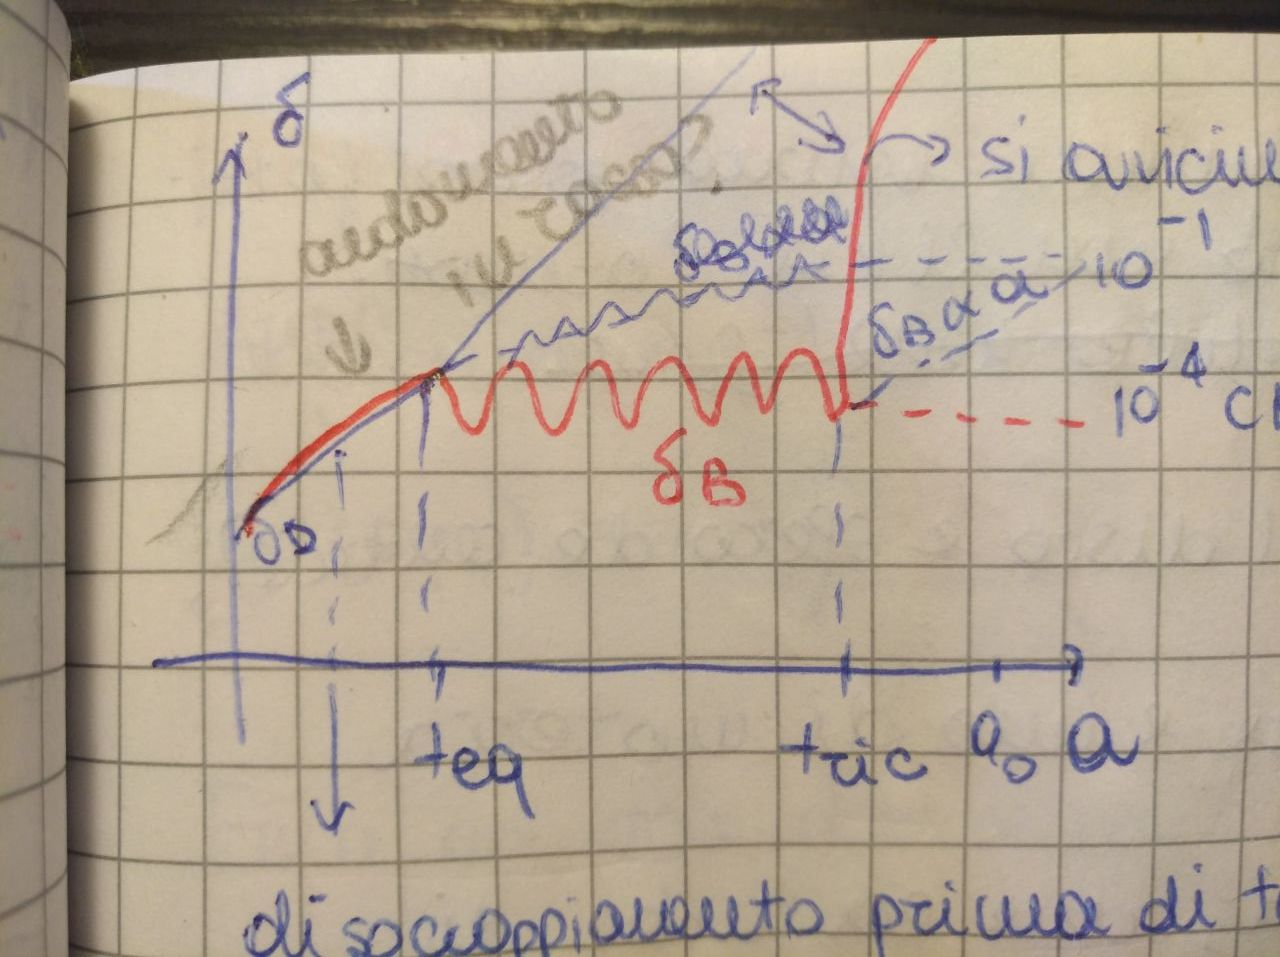
\includegraphics[width=7cm, height=7cm]{images/pertosc1.jpeg}
\caption{Andamento delle perturbazioni di materia barionica ed esotica in funzione di t.}
\label{fig:pertosc1}
\end{figure}
\begin{itemize}
\item \underline{$t<t_{eq}$}: materia oscura e barionica sono \textbf{accoppiate}, dunque le perturbazioni crescono allo stesso modo.
\item \underline{$t_{eq}<t<t_{ric}$}: ho il \textbf{disaccoppiamento}, quindi $\delta_D$ inizia a crescere. La materia baronica \'{e} ancora accoppiata ai fotoni ed oscilla poich\'{e} ancora al di sotto di $M_J$.
\item \underline{$t>t_{ric}$}: avviene il disaccoppiamento tra barioni e fotoni, mancando la forza di richiamo data da $P_{rad}$ la $M_J$ crolla e le perturbazioni di materia barionica collassano. Trovandosi in universo con perturbazioni di DM evolute, le perturbazioni barioniche collassano per autogravit\'{a} ed a causa della DM, fino a tendere asintoticamente al suo andamento.
\end{itemize}
Uno scenario con la DM \'{e} in accordo con i dati osservativi, senza avremmo dei contrasti di densit\'{a} di materia ordinaria molto pi\'{u} piccoli a queste scale ($10^2$ vs $10^{-1}$). \\
Non considerando l'argomento degli \textbf{elementi leggeri} che proverebbero la necessit\'{a} di una materia oscura non barionica \footnote{Come sottolinea il grafico che mostra che le due forme di materia si disaccoppiano.}, ipotizziamo una materia oscura barionica \textbf{MACHOs}\footnote{Massive Astrophysical Halo Object: BH, NS, BD.}. Si teorizzarono essere micro BH ($M\sim 1 M_\odot\ $)formatisi nell'universo primordiale a $ t<t_{eq}$, disaccoppiati da fotoni e dal resto della materia barionica esistente. In quanto oggetti massicci non luminosi dovrebbero essere responsabili dell'effetto di \textbf{lente gravitazionale} \footnote{Deformazione immagine; aumento della luminosit\'{a} (fotoni convergono) in tutte le frequenze.}. Negli anni '90 si avvi\'{o} una campagna osservativa di ricerca di questi oggetti nella nostra galassia, tuttavia non vennero osservati. La DM deve essere non barionica e \textbf{diffusa}.
\subsection{Modi per quantificare la struttura su larga scala: spettro delle perturbazioni}
Usando un approccio inverso rispetto al precedente, consideriamo la perturbazione di densit\'{a} funzione dello spazio e fissa nel tempo. Notiamo che su un volume abbastanza grande $\delta(\textbf{x})$ diventa periodico e quindi posso svilupparlo in \textbf{serie di Fourier}.
\begin{equation}
\delta(\textbf{x})=\sum_{\textbf{k}}\delta_{\textbf{k}}\exp{ikx}
\end{equation}
Integrando sul volume $\int \delta(\textbf{x})d\textbf{k}=0$ poich\'{e} l'universo a larga scala \'{e} omogeneo e isotropo. Dalla teoria sulla TF abbiamo che $\langle \sigma^2 \rangle =\sigma^2=\sum_{\textbf{k}} \mid \delta_{\textbf{k}}\mid^2$ in versione integrale $\sigma^2= \frac{1}{(2\pi)^3}\int \mid \delta_{\textbf{k}}\mid^2 d\textbf{k}$  fornisce l'ordine di grandezza delle perturbazioni; $\mid \delta_{\textbf{k}}\mid^2=P(\textbf{k})$ \'{e} definito \textbf{Spettro di Potenza} mi da l'ampiezza delle componenti corrispondenti ai diversi vettori d'onda, e quindi mi dice cosa domina nella serie. Anche se noi abbiamo visto che c'\'{e} dipendenza anche da $t$ e dunque $\delta(t)=D(t) \delta_i$ e dunque $P(\textbf{k},t)=D(t)P_i(\textbf{k})$, ipotizzando campo di densit\'{a} iniziale gaussiano $P(\delta_i) d\delta_i=\frac{1}{\sqrt{2\pi \sigma^2}}\exp{-\frac{\delta_i^2}{2\sigma^2}}d\delta_i$ . La perturbazione di densit\'{a} iniziale $\delta_i$ \'{e} una variabile aleatoria gaussiana, quindi una fluttuazione attorno al valor medio. La gaussiana \'{e} una densit\'{a} di probabilit\'{a} che ha due momenti non nulli: il valor medio che \'{e} nullo in caso universo omogeneo e isotropo, e la varianza che prendiamo come riferimento.  Questo vale solo se $\delta(\textbf{x})=\frac{\rho(\textbf{x})-\bar{\rho}}{\bar{\rho}}<<1$ ma deve valere per $\bar{\rho}$ abbastanza grande da calcolare la massa dell'universo e abbastanza piccolo per identificare $\rho(\textbf{x})$ quindi devo definire una scala $\delta (\textbf{x}, R)$. 
\begin{equation}
\begin{cases}
\sigma(R)^2= \frac{1}{2\pi^2}\int_0^{\infty} P(k) k^2 w(kR)^2 d\textbf{k}
\\
w(kR)=3\frac{\sin{kR}-\cos{kR}}{(kR)^3}
\end{cases}
\end{equation}
Definisco $w(kR)$ funzione filtro media l'informazione sulla scala a cui mi trovo: seleziona una sfera di raggio R su cui considerare il contrasto.
\subsubsection{Spettro instabile delle perturbazioni}
Considerando un \textbf{filtro gaussiano} e uno \textbf{spettro di potenza} per $P(k)$:
\begin{equation}
\begin{cases}
\sigma(R)^2= \frac{1}{2\pi^2}\int_0^{\infty} P(k) k^2 w(kR)^2  d\textbf{k}
\\
w_G(kR)=\exp{2\frac{k^2R^2}{2}}
\\
P(k)= Ak^n
\end{cases}
\label{eq:var}
\end{equation}
Ottengo $\sigma^2(R)=\frac{A}{4\pi^2}\Gamma\big(\frac{n+3}{2}\big)R^{-(n+3)}$: la varianza decresce con la scala, quando $R>>1$ l'universo \'{e} omogeneo e dunque $\delta\rightarrow 0 \Rightarrow \sigma\rightarrow 0$.\\
\textbf{Applicazione}: considerando un volume in cui vengono distribuite particelle massive randomicamente, la massa totale $M=mN$. Le fluttuazioni di particelle nei sotto-volumi di quello principale avranno distribuzione \textbf{Poissoniana} quindi $\sigma\propto N^{\frac{1}{2}}\propto M^{-\frac{1}{2}}$ siccome $m$ \'{e} la stessa. Il raggio e la massa sono legati dalla relazione $R\propto M^{\frac{1}{3}}$ che sostituendo nella legge della varianza in \ref{eq:var} mi  alla relazione sugli esponenti $n=0$. Questo mi da uno spettro di potenza \textbf{costante}, cio\'{e} \textbf{rumore bianco}: tutti i numeri d'onda contribuiscono allo stesso modo alla costruzione del campo di densit\'{a} iniziale.
\subsubsection{Spettro di potenza di Harrison-Zel'dovich}
Le fluttuazioni quantistiche nel periodo pre-inflattivo causano perturbazioni nel campo densit\'{a} che nel periodo post-inflattivo sar\'{a} perturbato secondo lo spettro di Harrison-Zel'dovich.\\
Immagino di essere $t<t_{eq}$ (radiation dominant) a scale cosmiche, quando le perturbazioni di densit\'{a} varcano l'orizzonte cosmologico:
\begin{equation}
\begin{cases}
M_H\propto a^3
\\
\sigma\propto a^2 M_H^{-\frac{n+3}{6}} 
\end{cases}
\end{equation}
Quindi otteniamo la seguente relazione di proporzionalit\'{a} $\sigma\propto M_H^{\frac{1-n}{6}} $. 
\begin{figure}[htp]
\centering
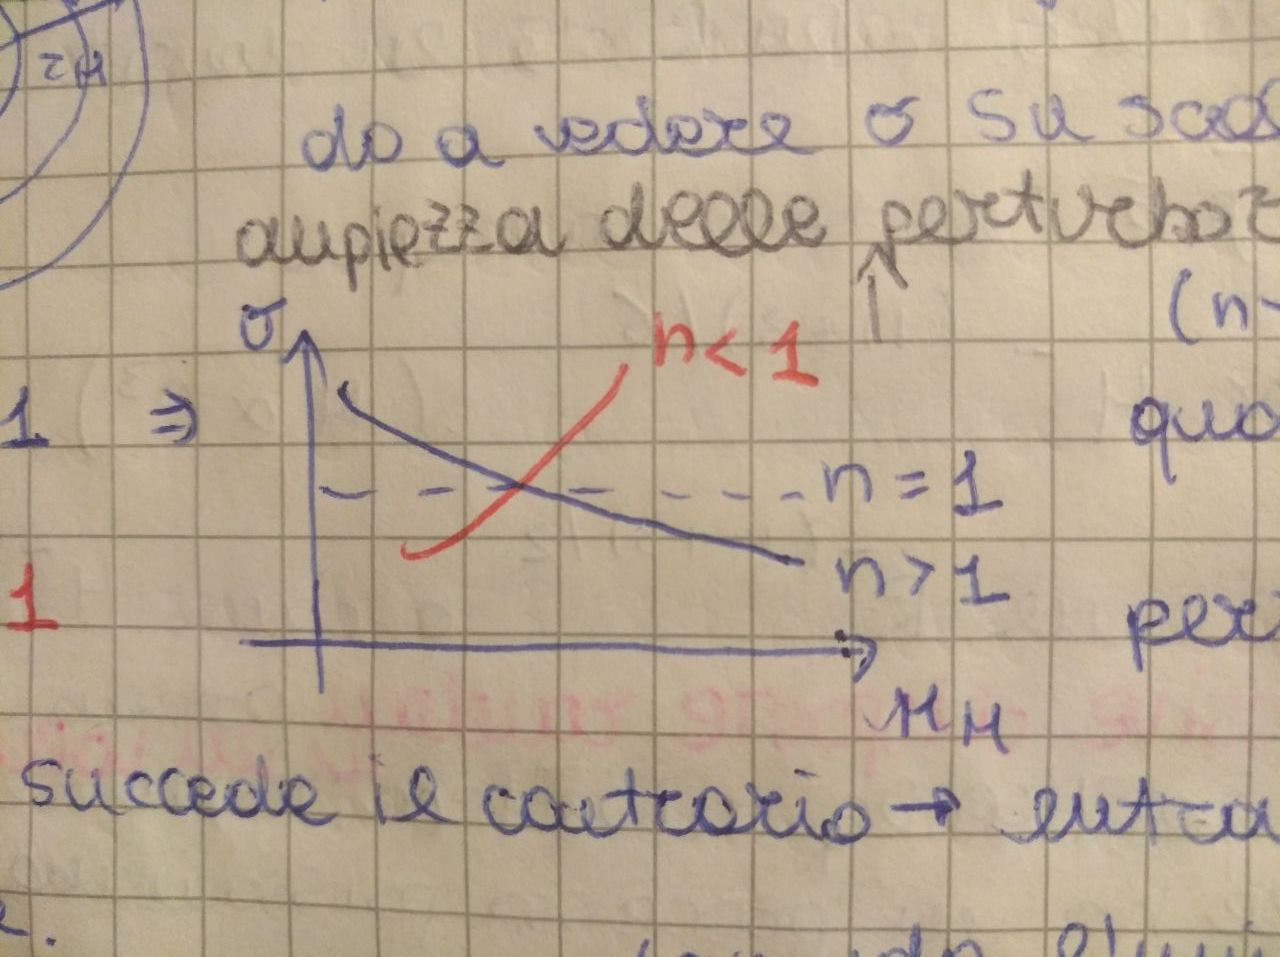
\includegraphics[width=7cm, height=7cm]{images/harrisonzeldovich.jpeg}
\caption{Andamento della varianza in funzione di $M_H$.}
\label{fig:harrisonzeldovich}
\end{figure}
\begin{itemize}
\item $n<1$: per $r>>1$ allora $\sigma \rightarrow \infty$ diverge. \textbf{Problema}: \'{e} in contrasto con un univ. \textbf{omogeneo} ed \textbf{isotropo} su larga scala. Si sarebbero creati i micro BH, ci\'{o} non succede tuttavia grazie alla radiazione di Hawking, che ritarda la nucleosintesi cosmologica.
\item $n>1$: per $M_H\rightarrow 0 $ allora $\sigma \rightarrow \infty$ diverge. \textbf{Problema}: mano a mano che entrano le perturbazioni la varianza dovrebbe decresce.
\item $n=1$: Harrisono e Zel'dovich deducono che espandendosi l'universo fa entrare perturbazioni sempre con la stessa varianza. Ci\'{o} produce uno spettro  lineare $P(k)=Ak$. 
\end{itemize}
Potremmo descrivere i problemi della divergenza di $\sigma$ attraverso il potenziale gravitazionale, dal momento che \'{e} correlato alle pert. di densit\'{a}.
\begin{equation}
\begin{cases}
\delta \phi \sim \frac{\delta M}{R}\propto k \delta M
\\
\sigma\propto \frac{\delta M}{M} \propto M^{-\frac{n+3}{6}}
\end{cases}
\end{equation}
Ho la relazione $\delta \phi \propto k^{\frac{n-1}{2}}$ ($k$ \'{e} la scala):
\begin{itemize}
\item $n<1$: diverge a piccoli $k$.
\item $n>1$: diverge a grandi $k$.
\item $n=1$: costante.
\end{itemize}
Quindi $n=1$, $n=0.97$ per essere precisi, diventa una predizione dei modello inflattivo. L'inflazione risolve i 3 problemi del modello HBB, ma avendo espanso su scale cosmiche le fluttuazioni su scale quantistiche dell'universo primordiale si crea un campo di densit\'{a} perturbato con 2 peculiarit\'{a}:
\begin{enumerate}
\item I contrasti di densit\'{a} $\delta$ sono delle variabili aleatorie gaussiane (ci basta $\sigma$ per descrivere il campo di densit\'{a}).
\item Ha lo spettro di potenza di HZ.
\end{enumerate}
Osservo che le perturbazioni su scala maggiore dell'orizzonte c. ($r>r_H$) corrispondono a perturbazioni del potenziale g. $\phi$ che sono congelate nella metrica stessa.
\subsubsection{Evoluzione delle perturbazioni adiabatiche nei modelli HDM e CDM}
Come evolve lo spettro di potenza HZ per le perturbazioni di densit\'{a} ($P(k)=\mid \delta_k\mid^2\propto k$) all'epoca dell'equivalenza $t_{eq}$, quando inizia ad agire il collasso per instabilit\'{a} gravitazionale?
Per un fluido non collisionale di materia oscura ho la scala di lunghezza FS che regola i processi, e dipende dalla velocit\'{a} peculiare delle particelle: cio\'{e} quando diventano relativistiche. Quando le perturbazioni entrano nell'orizzonte, in un universo in espansione, se $M<M_{FS}$ allora possono crescere per instabilit\'{a} gravitazionale. Lo spettro di $P(k)$ sar\'{a} cambiato soprattutto su piccole scale, causa della lunghezza d'onda di FS al tempo dell'equivalenza: $\lambda_{eq}=\frac{ct_{eq}}{a_{eq}}=13(\Omega_0 h^{-2})^{-1}Mpc$. In base al valore di $M_{FS} \propto r_{FS}^3$ ho una materia oscura diversa:
\begin{itemize}
\item $r_{FS}\sim \lambda_{eq} (=100 Mpc) \Rightarrow$ HDM (neutrini): quindi al di sotto di questa scala (ammassi di galassie $M_{FS}\sim 10^{14}-10^{15} M_\odot\ $) le perturbazioni vengono spazzate via, perch\'{e} le strutture su piccola scala si formano per frammentazione delle perturbazioni su larga scala. Lo spettro si smorza su  piccola scala ($k>>1$).
\item $r_{FS}<< \lambda_{eq} (=1 Mpc) \Rightarrow$ CDM: la potenza delle perturbazioni decrescono a scale ancora pi\'{u} piccole, le particelle diventano non relativistiche molto presto. Il modello non essendo influenzato da $r_{FS}$ permette la crescita di perturbazioni su scale pi\'{u} piccole, permettendo una gerarchia \textbf{bottom-up}.
\item $r_{FS}\sim \lambda_{eq} (=1 Mpc) \Rightarrow$ WDM: cade tra i due estremi.
\end{itemize}
\begin{figure}[htp]
\centering
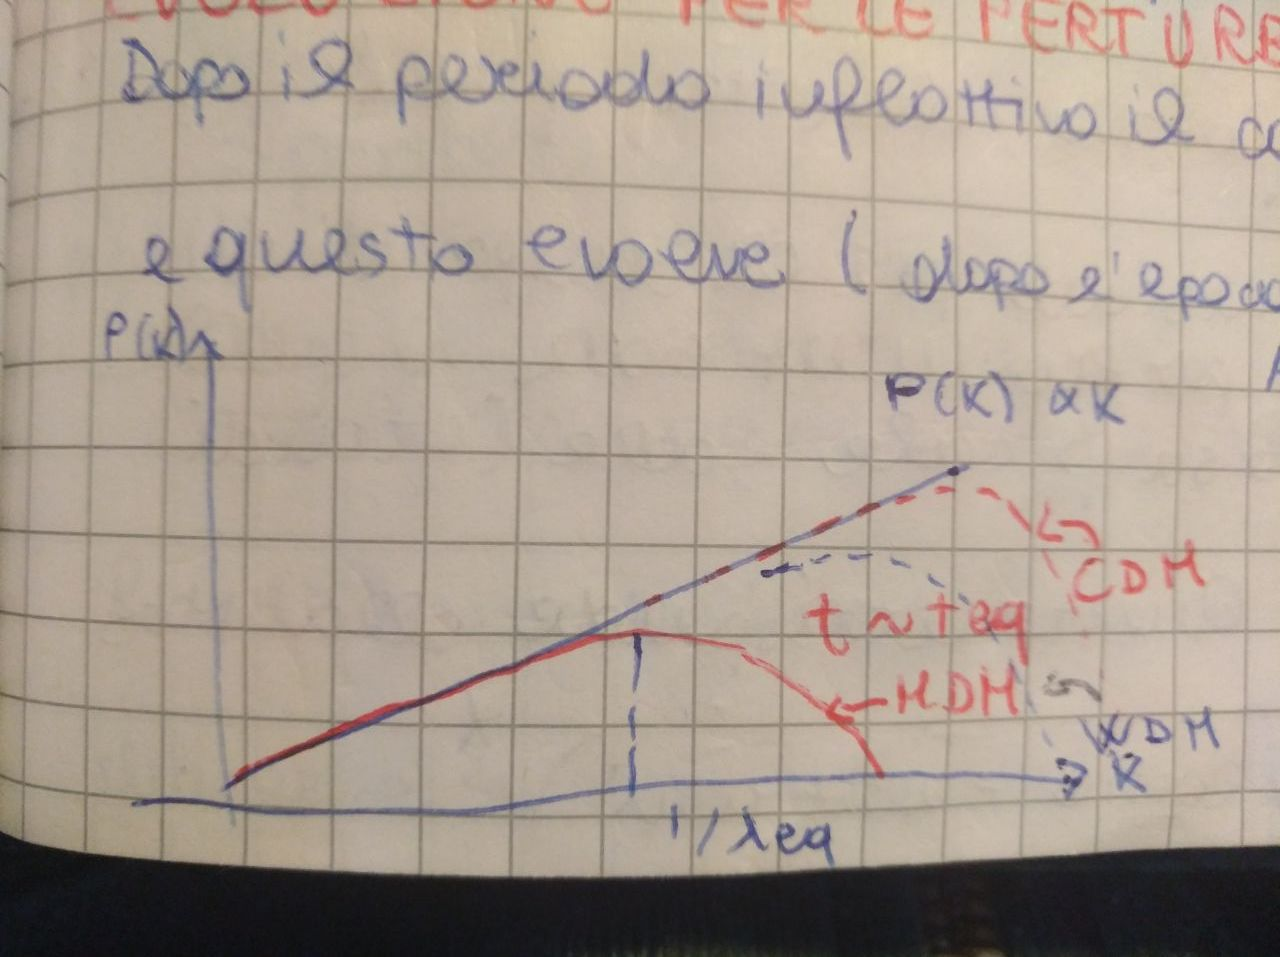
\includegraphics[width=7cm, height=7cm]{images/cdm.jpeg}
\caption{Evoluzione della potenza in funzione della scala per modelli di DM a confronto.}
\label{fig:cdm}
\end{figure}
Ricapitolando l'ampiezza delle perturbazioni decrescono pi\'{u} rapidamente alle grandi scale (per tutti i modelli di DM). Secondo la gerarchia \textbf{bottom-up} le perturbazioni crescono alle piccole scale, in cui \textbf{viralizzano} (dynamical friction in cui lo scambio di energia avviene per interazione gravitazionale) nella fase non lineare evolvono verso configurazioni di equilibrio in cui le masse hanno la stessa distribuzione di velocit\'{a}. Successivamente comincia il processo di \textbf{merging} influenzato dalle perturbazioni su larga scala.\\
Usando L'equazione cinetica di Boltzmann per un fluido di DM in un universo in espansione (nello spazio delle fasi) deriviamo lo spettro di potenza dell'epoca dell'equivalenza essere:
\begin{equation}
\begin{cases}
P_{eq}(k)=T^2(k)P_i(k)
\\
T_{CDM}=\left\{   1+\big[ \frac{ak}{\Gamma}+(\frac{bk}{\Gamma})^{\frac{3}{2}}+(\frac{ck}{\Gamma})^2\big]^{\nu}  \right\}^{-\frac{1}{\nu}}
\end{cases}
\end{equation}
Con $T^2(k)$ \textbf{funzione di trasferimento}, dipendente dal modello di DM che scegliamo quindi da $r_{FS}$, e $\Gamma=\Omega_0 h$ \textbf{parametro di forma}. \\
Dal campo di densit\'{a} oggi abbiamo informazioni sul tipo di DM (se misuro $P\rightarrow T\rightarrow \Omega$). Quindi l'universo su larga scala ci da un sacco di informazioni sulla  materia presente nell'universo. Conosciamo la relazione $P_0(t,k)=D^2(t)P_{eq}(k,t'<t)$, ma abbiamo 3 problemi:
\begin{enumerate}
\item Vale solo su scale lineari cio\'{e} dove $\delta<<1$ ovvero su larga scala ($>10Mpc$).
\item $D(t)$ contiene $\Omega_0$ quindi devo conoscere il modello cosmologico.
\item Ho bisogno di conoscere la distribuzione su larga scala dell'universo, attraverso cataloghi di galassie (time consuming).
\end{enumerate}
\subsubsection{Crescita non lineare delle perturbazioni di densit\'{a}}
Zel'dovich propone un approccio analitico per studiare le perturbazioni di densit\'{a}:
\begin{itemize}
\item $1°$ approx. di Z. ($\delta <<1$): teoria lineare
\item $2°$ approx. di Z. ($\delta>>1$): teoria non lineare, siamo su scale galattiche  a $\delta\sim 10^6$ \footnote{Permette di costruire un ponte tra la $P_{eq}$ e $P_0$ su scale non lineari.}.
\end{itemize}
Consideriamo l'evoluzione lineare delle perturbazioni di densit\'{a}:
\begin{equation}
\begin{cases}
\delta(t)=D(t) \delta_i
\\
\dot{\mathbf{u}}+2\frac{\dot{a}}{a}\mathbf{u}=-\frac{1}{a^2}\nabla_x \phi_1
\end{cases}
\end{equation}
Inserendo la velocit\'{a} peculiare $\mathbf{v}=a\mathbf{u}$ e tenendo conto dell'equazione di \textbf{Poisson} (riespressa considerando la conservazione del tensore E-I) $\nabla_x^2\phi_1=\nabla_x^2\phi_0 \frac{D}{a}$  integrando una volta si opttiene:
\begin{equation}
\mathbf{v}=-\frac{1}{a} \left [ \int \frac{D}{a}dt\right ]\nabla_x \phi_0 + \mathbf{v}_0
\end{equation}
Come condizione iniziale sulla velocit\'{a} consideriamo $v_0=0$. Si fa notare che l'approssimazione sta nel considerare la perturbazione del potenziale costante nel tempo. Introducendo il tempo conforme $d\tau=\frac{dt}{a}$ si risale alle coordinate:
\begin{equation}
\mathbf{x}=\mathbf{x}_0-\left [ \int \frac{d\tau}{a}\int D d\tau\right ]\nabla_x \phi_0 
\end{equation}
Rimaneggiando l'equazione di evoluzione delle perturbazioni notiamo:
\begin{equation}
\int \frac{d\tau}{a}\int D d\tau=\frac{\delta}{4 \pi G \rho a^3 \delta_i}
\end{equation}
In fine abbiamo il set di equazioni definitivo \footnote{Si nota la dipendenza dalle accelerazioni costanti iniziali.}:
\begin{equation}
\begin{cases}
\mathbf{x}=\mathbf{x}_0- \frac{D(\tau)}{4 \pi G \rho a^3}\nabla_x \phi_0 
\\
\mathbf{v}=- \frac{\frac{dD}{d\tau}}{4 \pi G \rho a^3}\nabla_x \phi_0 
\end{cases}
\end{equation}
Quindi data una perturbazione non sferica, immaginando che il campo di accelerazione sia costante nel tempo ($\nabla_x \phi_0 \sim cost$) \footnote{In realt\'{a} non \'{e} cos\'{i} perch\'{e} cambiando le posizioni della materia cambia anche il potenziale.} 
\begin{itemize}
\item le particelle si muoveranno lungo rette $v\propto \nabla\phi$ verso il contrasto di densit\'{a} pi\'{u} alto (direzione e velocit\'{a} costante). 
\item Esistendo direzioni fissate ne avremo una che apporta materia pi\'{u} velocemente rispetto alle altre, quindi abbiamo una direzione di collasso preferenziale che porta alla formazione di un piano.
\item Segue il fenomeno dello \textbf{shell crossing}, o pi\'{u} semplicemente attraversamento, ovvero quando le particelle attraversano il piano, la mappatura tra $x_0$ e $x$ non \'{e} pi\'{u} univoca.
\end{itemize}
Quindi la $1°$ approx. di Z. non \'{e} pi\'{u} valida, siamo nel regime non lineare. Possiamo estendere tale approccio anche al caso non lineare a contrasti di densit\'{a} molto elevati con risultati abbastanza accurati. Per\'{o} ora focalizziamoci sull'approccio computazionale usato gi\'{a} a partire dagli anni '80.
\subsubsection{Soluzioni numeriche}
Le simulazioni numeriche costituiscono l'unico riscontro sperimentale di cui la cosmologia pu\'{o} avvalersi. Supponiamo ora  di avere una scatola piena di un fluido continuo, che rappresenta certamente l'universo. Esistono due differenti approcci con cui studiare il sistema:
\begin{enumerate}
\item \textbf{Euleriano (pti. densit\'{a})}: vale alle larghe scale ($100 Mpc$) e consiste nel rappresentare il campo di densit\'{a} attraverso dei punti griglia. \underline{Con:} bassa risoluzione poich\'{e} non vado al di sotto della maglia pi\'{u} fine. \underline{Pro:} basso tempo di calcolo. 
\item \textbf{Lagrangiano (pti. massa)}: vale su piccole scale e consiste nel rappresentare la materia come punti massa. \underline{Con:} alti tempi di calcolo poich\'{e} devo risolvere N equazioni differenziali ($t\sim N^2$). \underline{Pro:} alta risoluzione nel caso di alta densit\'{a} di particelle. Queste si chiamano soluzioni a N-corpi.
\item \textbf{Ibridi}: vengono mescolati i due precedenti approcci per ottenere il migliore risultato.
\item \textbf{Tree code}: ho delle macro-particelle che aggiorno meno frequentemente.
\end{enumerate}
Chiaramente ognuno dei metodi citati dipende dalle variabili di sistema: N particelle, volume, risoluzione spaziale...
\subsubsection{Problemi numerici}
Le condizioni iniziali su posizioni e velocit\'{a} costituiscono il vero problema delle simulazioni cosmologiche. Le posizioni iniziali devono descrivere il campo di densit\'{a} iniziale $\delta$ che espanso in serie di Fourier mi da i coefficienti $\mid \delta_k\mid^2=P(k)=T^2(k)P_i(k)$ esprime l'entit\'{a} della fluttuazione media. Quindi scelgo le condizioni iniziali in modo che mi riproducano lo spettro CDM $P(k)$.\\
Ricapitolando, la teoria lineare funziona da $z\sim 10^3-10^4$ fino a $z\sim 20$ in cui abbiamo i primi fenomeni di attraversamento. Allora facciamo partire da qui la simulazione scegliendo le condizioni iniziali secondo il metodo descritto poc'anzi, e facendo evolvere il sistema fino a $z\sim 0$, quindi avr\'{o} delle strutture che comparo con le osservazioni.\\
Prendiamo ad esempio le simulazioni \textbf{ibride}. Dobbiamo modellizzare 3 tipi di fluidi differenti:
\begin{itemize}
\item materia barionica stellare
\item materia barionica gassosa
\item materia non barionica (DM)
\end{itemize}
di cui ognuna ha delle propriet\'{a} fisiche differenti. Quella barionica \'{e} collisionale dunque:
\begin{itemize}
\item ha un termine di pressione
\item si raffredda in modo \textbf{termico} e \textbf{radiativo}
\item istabilit\'{a} gravitazionale: collassa formando degli oggetti stellari non collisionali
\end{itemize}
La materia oscura \'{e} non collisionale e interagisce solo \textbf{gravitazionalmente}, dunque non \'{e} soggetta a nessun tipo di "cooling", quindi non dissipa energia. Un'altra complicazione di cui si deve tenere conto \'{e} per giunta il processo di raffreddamento, che si sviluppa su scale atomiche. Quindi abbiamo un problema di \textbf{scala}, infatti passiamo da scale cosmiche a scale nanoscopiche.\\
Le simulazioni a gravit\'{a} Newtoniana e CDM sono concordi con le osservazioni, abbiamo dunque delle strutture su larga scala comparabili. I neutrini dunque non potevano costituire la materi oscura dominante.
\newpage
\section{Cosmologia osservativa}
\subsection{Funzione di correlazione a due punti}
Introduciamo questo strumento per confrontare la distribuzione di materia su larga scala con quella prevista dai modelli di DM. Definiamo $dP=\boxed{\bar{n}^2}\boxed{(1+\Sigma(r))}dV_1 dV_2$ come la probabilit\'{a} di trovare una particella che definisce il volumetto $dV_2$ ad una distanza $r$ rispetto alla particella che definisce il volumetto $dV_2$. Il termine $dP\propto \bar{n}^2$ costituisce una Poissoniana, mentre il termine dipendente dalla scala $dP\propto(1+\Sigma(r))$ indica la di quanto ci si scosta dalla distribuzione, qui compare la \textbf{Funzione di Correlazione} $\Sigma(r)$.\\
Cerco una correlazione tra $\delta$ e $\Sigma$ partendo dall'approssimazione a \textbf{fluido continuo} di una distribuzione di punti un cui la densit\'{a} \'{e} definita $\rho(\bar{x})=\bar{\rho}+ [1+\delta(\bar{x})]$. Arriviamo ad esplicitare la funzione di correlazione come funzione di coovarianza delle $\delta$ come
\begin{equation}
\Sigma(\bar{r})=\langle \delta(\bar{x}) \delta(\bar{x}+\bar{r})\rangle_{\bar{x}}
\end{equation}
Sostituendo lo sviluppo di Fourier otteniamo che codesta funzione \'{e} la \textbf{TF dello spetto di Potenza}.
\begin{equation}
\begin{cases}
\Sigma(\bar{r})=\frac{1}{(2\pi)^3}\int P(\mathbf{k})\exp{-i\mathbf{k}\mathbf{r}}d^3k
\\
P(\mathbf{k})=\frac{1}{(2\pi)^3}\int \Sigma(r)\exp{i\mathbf{k}\mathbf{r}}d^3r
\end{cases}
\end{equation}
\textit{Come confronto la distribuzione di galassie su larga scala con i modelli?}\\
\textbf{Premesse}:
\begin{itemize}
\item Ho la distribuzione di galassie oggi a $z=0$, su scale non lineari.
\item Il modello CDM ci da la distribuzione all'equivalenza.
\end{itemize}
Una via \'{e} quella delle simulazioni a N-corpi. Dunque parto dallo spettro inflattivo all'equivalenza che ottengo approssimazione lineare
\begin{equation}
\begin{cases}
P_i(k)=Ak
\\
P_{eq}(k)=T_{mod}^2(k)P_i(k)
\end{cases}
\end{equation}
Lo spettro di potenza nel regime non lineare \'{e} legato a quello nel regime lineare attraverso una funzione analitica, ricavata dalle simulazioni e dipendente dal modello usato. Questa approssimazione porta ad una sottostima dell'entit\'{a} della perturbazione, noi consideriamo l'approccio numerico.\\
Per poi arrivare a determinare $P(k,t)$ (sapendo che $P=\mid \delta_k\mid^2$ e $\langle \delta^2 \rangle \propto D^2$), tramite il modello matematico proposto poc'anzi:
\begin{enumerate}
\item Trovo i punti attraverso la simulazione.
\item Misuro la funzione di correlazione.
\item TF ottenendo lo spettro di potenza a tutti i tempi.
\end{enumerate}
Dallo spettro di potenza che simulo riesco a risalire alla funzione di correlazione facendo la TF.
\begin{equation}
P_{gal}(k) \longrightarrow \Sigma_{gal}(r)
\end{equation}
Il modello CDM \'{e} in accordo con le osservazioni, le barre di errore lasciano spazio ad una possibile percentuale non nulla di WDM e HDM. Confrontando il modello su larga scala con le misurazioni possiamo stimare $\Omega_0$, che \'{e} contenuta infatti nella relazione dello spettro di potenza $T_{CDM}\propto (\Gamma=\Omega_0 h)$. Otteniamo un $\Gamma\sim 0.21$ tale che $\Omega_0 \sim 0.3$.
\subsubsection{Insigth sull'evoluzione delle perturbazioni}
Le strutture crescono linearmente con il tempo, indipendentemente dalla scala. Ma su scale sufficientemente piccole lo spettro di potenza stimato con approssimazione lineare \'{e} una sottostima di quello reale. Il processo di formazione delle strutture \'{e} altamente non lineare e questi effetti ne aumento il rate di crescita. Dall'approssimazione di Zel'dovich si evince che le particele si muovono su linee rette fino all'attraversamento, qui essendo pi\'{u} vicine risentono dell'attrazione gravitazione che le rallenta nel loro moto e le fa collassare. La non linearit\'{a} aumenta la rapidit\'{a} con cui una perturbazione cresce.
\subsubsection{Misura della funzione di correlazione}
Negli anni '80 l'universo era mappato unicamente a bassi $z$, si conosceva infatti la \textbf{sfera celeste}. Invece di misurare $\Sigma(r)$, funzione di correlazione che corrisponde ad una conoscenza della distribuzione della materia nello spazio, si riusciva a misurare $W(\theta)$ che corrisponde ad una separazione angolare degli oggetti. La relazione tra le due funzioni si ricava imponendo l'Isotropia nella distribuzione di galassie su larga scala: $dP=\bar{n}_{\Omega}^2 [1+W(\theta)] d\Omega_1 d\Omega_1$. Dopo alcuni passaggi si arriva alla definizione di $W(\theta)\propto \theta^{1-\gamma}$ che porta a $\Sigma(r)=(\frac{r}{r_0})^{-\gamma}$ con $\gamma=1.8$ e $r_0=5 \frac{Mpc}{h}$:
\begin{itemize}
\item $\Sigma \rightarrow 0$ per $r\rightarrow \infty$: le galassie hanno distribuzione Poissoniana su larga scala ($100Mpc$).
\item $\Sigma \rightarrow 1$ per $r\rightarrow r_0$: ho una probabilit\'{a} doppia di trovare due galassie a questa distanza rispetto ad una distribuzione Poissoniana ($10Mpc$) \footnote{Questo ultima istanza \'{e} a favore della tesi sulla formazione delle strutture per instabilit\'{a} gravitazionale.}.
\end{itemize}
\underline{Metodo 1°}: una possibile stima di $\Sigma$ su scala galattica ($10Mpc$) consiste nel sovrapporre ad una distribuzione di galassie 2D reale una casuale, e studiare il rapporto tra il numero di coppie coppie di galassie a distanza $r$ reali e il rispettivo numero nella distribuzione casuale.
\begin{equation}
\begin{cases}
1+\frac{DD(\theta)}{DR(\theta)}=W(\theta)
\\
1+\frac{DD(r)}{DR(r)}=\Sigma(r)
\end{cases}
\end{equation}
\underline{Metodo 2°}: quando il numero di galassie su larga ($100Mpc$) scala diventa sufficientemente ampio, possiamo misurare $\Sigma$ nello spazio dei red shift, considerandola una velocit\'{a}, facendo uso della della legge di Hubble $cz=H_0d+v_{pec}$. Considerando due velocit\'{a} (misurate dallo spostamento verso il rosso dello spettro) di cui considero $v_2$ diretto lungo la los, si ha:
\begin{equation}
\begin{cases}
\mathbf{s}=\mathbf{v}_1-\mathbf{v}_2
\\
\mathbf{l}=\frac{\mathbf{v}_1+\mathbf{v}_2}{2}
\\
\mathbf{\pi}=\frac{\mathbf{s}\cdot\mathbf{l}}{_l}
\end{cases}
\end{equation}
Da cui si pu\'{o} facilmente calcolare $\mathbf{r}_p=\sqrt{s^2-\pi^2}$ distanza peculiare delle due galassie \textbf{ortogonale} alla los.
\begin{equation}
\int \Sigma(r_p, \pi) d\pi= W(r_p)=W(\theta)
\end{equation}
La funzione a due variabili $\Sigma(r_p, \pi)$ ha un \textbf{eccesso di correlazione}:
\begin{itemize}
\item $\pi>>1 \bigwedge r_p=0$
\item $r_p>>1 \bigwedge \pi=0$
\end{itemize}
Tale risultato quantifica un effetto che nello \textbf{spazio dei red shift} vediamo chiaramente. Se consideriamo una \textbf{red shift survay} di un \textbf{ammasso} si nota che assume una forma oblunga nella direzione della los, alcune galassie sono spostate a distanze maggiori. L'ammasso \'{e} circondato da galassie che "cadono" nella sua buca di potenziale, queste assumono $v_{pec}$ molto pi\'{u} basse di quelle dell'ammasso (che calcoliamo attraverso il Teorema del Viriale), poich\'{e} hanno $v_{pec}\parallel$ alla los (nel nostro riferimento solidale con l'ammasso) per cui a noi risulter\'{a} molto piccola o anche nulla. Quindi la parte centrale \'{e} costituita da galassie appartenenti all'ammasso, mentre la parte esterna sono galassie in \textbf{inflow}. A distanze proiettate piccole posso avere galassie con $\pi>>1$ (differenza di velocit\'{a} grande). Questo effetto di $\Sigma$ su piccola scala \'{e} dovuto alla presenza di sovradensit\'{a} che allunga i contorni abbiamo un \textbf{eccesso di correlazione}. Questa distorsione dello spazio dei red shift \'{e} un effetto non lineare che possiamo sfruttare per ricavare la densit\'{a} dell'universo senza conoscere necessariamente la $v_{pec}$ in quanto ho $\pi$:
\begin{equation}
v_{pec}\propto \underbrace{\frac{\Omega^{0.6}}{b}}_{\beta}\delta_{gal}
\end{equation}
Basta avere una \textbf{galaxy red shift survay} e descriverne la sua distorsione per avere informazioni sulla densit\'{a} dell'universo, che risulta essere $\Omega\sim 0.3$ per $b\sim 1$.
\subsubsection{Collasso di una perturbazione a simmetria sferica}
Considero una perturbazione sferica (3 autovalori uguali) con una discontinuit\'{a} a gradino \textbf{top hat}. Ne considero l'evoluzione temporale della perturbazione come se fosse un universo EdS dal momento che $\Omega(t_i)\sim1$ e $\Omega_{\Lambda0}(t_i)\sim 0$ in tempi remoti ($t_i>>1$), ed essendo omogenea viene descritta dall'equazione di Friedmann.
\begin{equation}
\begin{cases}
\delta(t_i)=\delta_{+}(t_i) (\frac{t}{t_i})^{\frac{2}{3}}+\underbrace{\delta_{-}(t_i)(\frac{t}{t_i})^{-1}}_{\rightarrow 0}
\\
\big(\frac{\dot{a}}{a}\big)^2=H_i^2\big[\frac{a_i}{a}\Omega_p(t_i)+1-\Omega_p(t_i)\big]
\end{cases}
\end{equation}
\begin{figure}[htp]
\centering
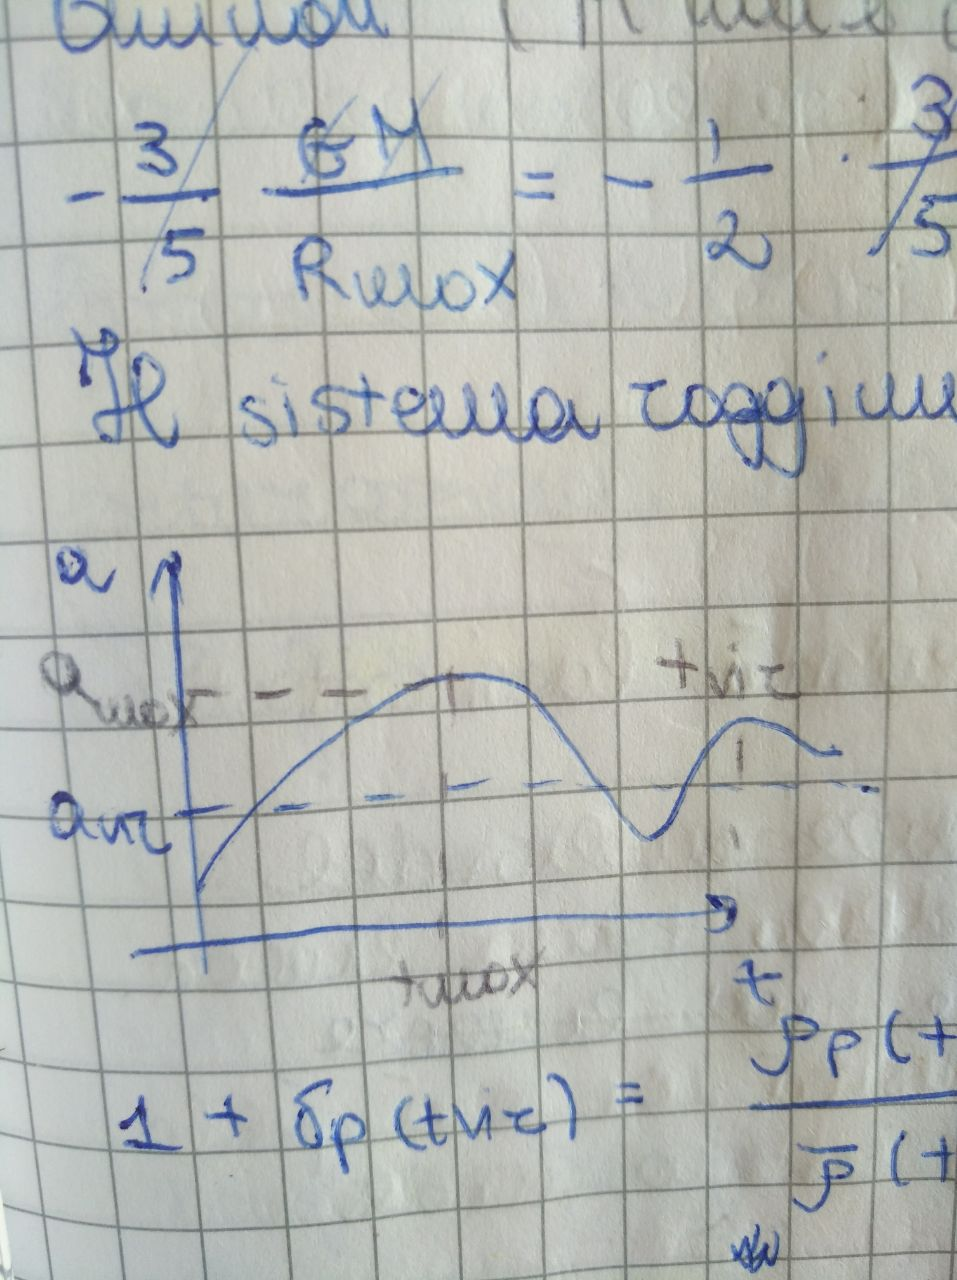
\includegraphics[width=7cm, height=7cm]{images/tophat.jpeg}
\caption{Evoluzione della perturbazione sferica con discontinuit\'{a} top hat.}
\label{fig:tophat}
\end{figure}
\begin{enumerate}
\item La perturbazione si \textbf{espande}, come un univ. di F, raggiungendo il suo massimo (sotto condizione: $\dot{a}_{max}=0, t=t_{max}$):
\begin{itemize}
\item $\rho_p(t_{max})=\frac{3\pi}{32 G t^2_{max}}$
\item $\delta_p(t_{max})\sim 4.6$ (la pert. ha una sovradensit\'{a} 5 volte maggiore alla densit\'{a} media dell'universo, la sua espanzione \'{e} rallentata dall'attraz. grav.).
\end{itemize}
\item La perturbazione \textbf{collassa} infatti abbiamo $\delta_i>\frac{1-\Omega_0}{\Omega_0(1+z_i)}$, ma non arriva mai a toccare $a_p=0$ (questo vale sia per perturbazioni barioniche e non):
\begin{itemize}
\item \textbf{materia barionica}: per il teorema del viriale nel momento in cui la materia collassa l'energia del potenziale gravitazionale viene trasformata in energia termica per irraggiamento, in dipendenza delle caratteristiche del potenziale, la pressione di radiazione si opporr\'{a} al collasso.
\item \textbf{materia oscura}: l'energia gravitazionale in questo caso viene trasformata in energia cinetica, non essendo collisionale questa energia si conserva secondo $ E+W=cost $: abbiamo trasformazioni $K \rightleftarrows W$. Il sistema non riesce a contenere le particelle (come fenomeno di FS), si aggrega in gusci di materia a velocit\'{a} non omogenee, abbiamo fenomeno di shell crossing. 
\end{itemize}
\item Il sistema \textbf{virializza}, si stabilizza, a $t_{vir}=2t_{max}$ tutti i gusci hanno velocit\'{a} nulla ($K=0 \Rightarrow E_{vir}= -\frac{1}{2}\mid W_{vir}\mid $). Si pu\'{o} dimostrare che l'energia potenziale gravitazionale di una sfera omogenena \'{e} $W=-\frac{3}{5}\frac{GM^2}{R}$. La sovradensit\'{a} $\delta_p $ cresce col tempo poich\'{e} $\bar{\rho}$ decresce con l'espansione dell'universo, fino a toccare a $t_{vir}$ il valore di 178: cio\'{e} \'{e } 200 volte pi\'{u} densa dell'universo. Si \'{e} in forte non linearit\'{a}.
\end{enumerate}
\'{E} interessante notare come l'approssimazione lineare avrebbe fallito, infatti avrebbe predetto un $\delta_{lin}\sim 1.68$ che \'{e} un sottostima di 2 ordini di grandezza. Questo ci pu\'{o} tornare utile in quanto potremmo estrapolare i valori di $\delta_{lin}$ della perturbazione di densit\'{a}, le propriet\'{a} statistiche restano valide nonostante non sia corretto il campo di densit\'{a}.\\
In generale il campo di densit\'{a} che evolve in un regime non lineare, alcune sovradensit\'{a} sono pi\'{u} virializzate di altri e le strutture su larga scala le connettono. 
\subsection{Teoria di Press-Schechter e funzione di massa}
Vediamo ora quante oggetti di massa M per unit\'{a} di volume sovradensi sono virializzati ad una certa epoca. Consideriamo $\delta$ una variabile aleatoria gaussiana che definisce la densit\'{a} di probabilit\'{a} delle perturbazioni di densit\'{a}:
\begin{equation}
\begin{cases}
P(\delta)d\delta=\frac{1}{\sqrt{2\pi}\sigma(M)}\exp{-\frac{\delta^2}{2\sigma^2(M)}}d\delta
\\
F(M)=\int_{\delta_c}^{\infty}P(\delta)d\delta
\end{cases}
\end{equation}
Dove la funzione $F(M)$ definisce la probabilit\'{a} che una perturbazione con $\delta>\delta_c$ di massa $M=\frac{4\pi}{3}\bar{\rho} R^3$ sia collassata all'epoca considerata. Il filtro gaussiano riduce l'esponenziale a 1 qualora la massa tenta a zero dunque la varianza esploda. Per mantenere la la normalizzazione (risolvendo l'integrale gaussiano) imponiamo un fattore moltiplicativo alla funzione che descrive il numero di oggetti di massa compresa tra $M$ ed $M+dM$ seguente:
\begin{equation}
N(M) dM=\boxed{2}\frac{\bar{\rho}}{M}\biggl|\frac{\partial F}{\partial M}\biggr| dM
\end{equation}
Facendo le dovute sostituzioni si arriva allo sviluppo dipendente anche da t:
\begin{equation}
N(M,t) dM=\frac{2}{\pi}\frac{\bar{\rho \delta_c}}{M \sigma^2(M,t)}\biggl|\frac{\partial \sigma}{\partial M}\biggr|\exp{-\frac{\delta_c^2}{2\sigma^2(M)}} dM
\end{equation}
La \textbf{funzione di massa} contiene una grande quantit\'{a} di informazioni:
\begin{itemize}
\item sullo spettro di potenza (informazione contenuta in $\sigma$)
\item sull'evoluzione lineare delle perturbazioni, ci\'{o} mi da informazioni su $D(\Omega_0)$
\end{itemize}
Si deduce che la funzione di densit\'{a} permette di vincolare il modello cosmologico (dal punto di vista del modello di universo di F.) sia il modello sulle perturbazioni di densit\'{a} poich\'{e} ne vincola lo spettro di potenza. Mediando con un filtro gaussiano la varianza si ha $\sigma (M,t)=AD(t)M^{-\frac{n+3}{6}}$  da cui:
\begin{equation}
n(M)dM=\frac{1}{\sqrt{2\pi}}\frac{\bar{\rho}}{M^2}\biggl(1+\frac{n}{3}\biggr)\biggl(\frac{M}{M^{\star}}\biggr)^{\frac{n+3}{3}} \exp{-\frac{1}{2}\biggl(\frac{M}{M^{\star}}\biggr)^{\frac{n+3}{3}}} dM
\end{equation}Confronto quantitativamente il modello della funzione di Press-Schechter in funzione del tempo considerando diversi modelli di universo di Friedmann (in figura riporto i valori limite.) con i dati osservativi.
\begin{figure}[htp]
\begin{minipage}[b]{8.5cm}
\centering
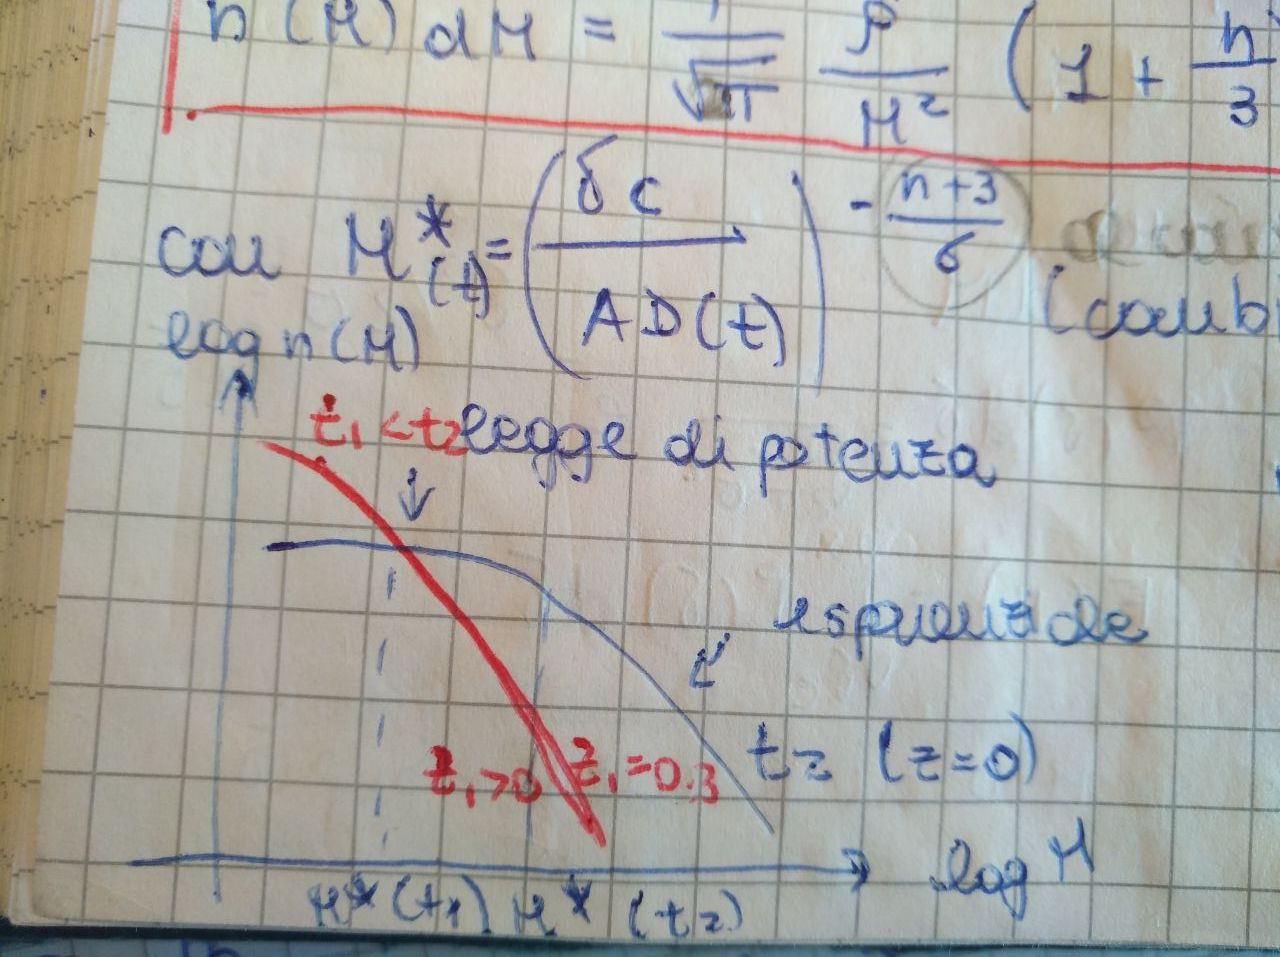
\includegraphics[width=8cm]{images/schechter.jpeg}
\caption{Funzione di massa di Schechter.}
\end{minipage}
\ \hspace{2mm} \hspace{3mm} \
\begin{minipage}[b]{8.5cm}
\centering
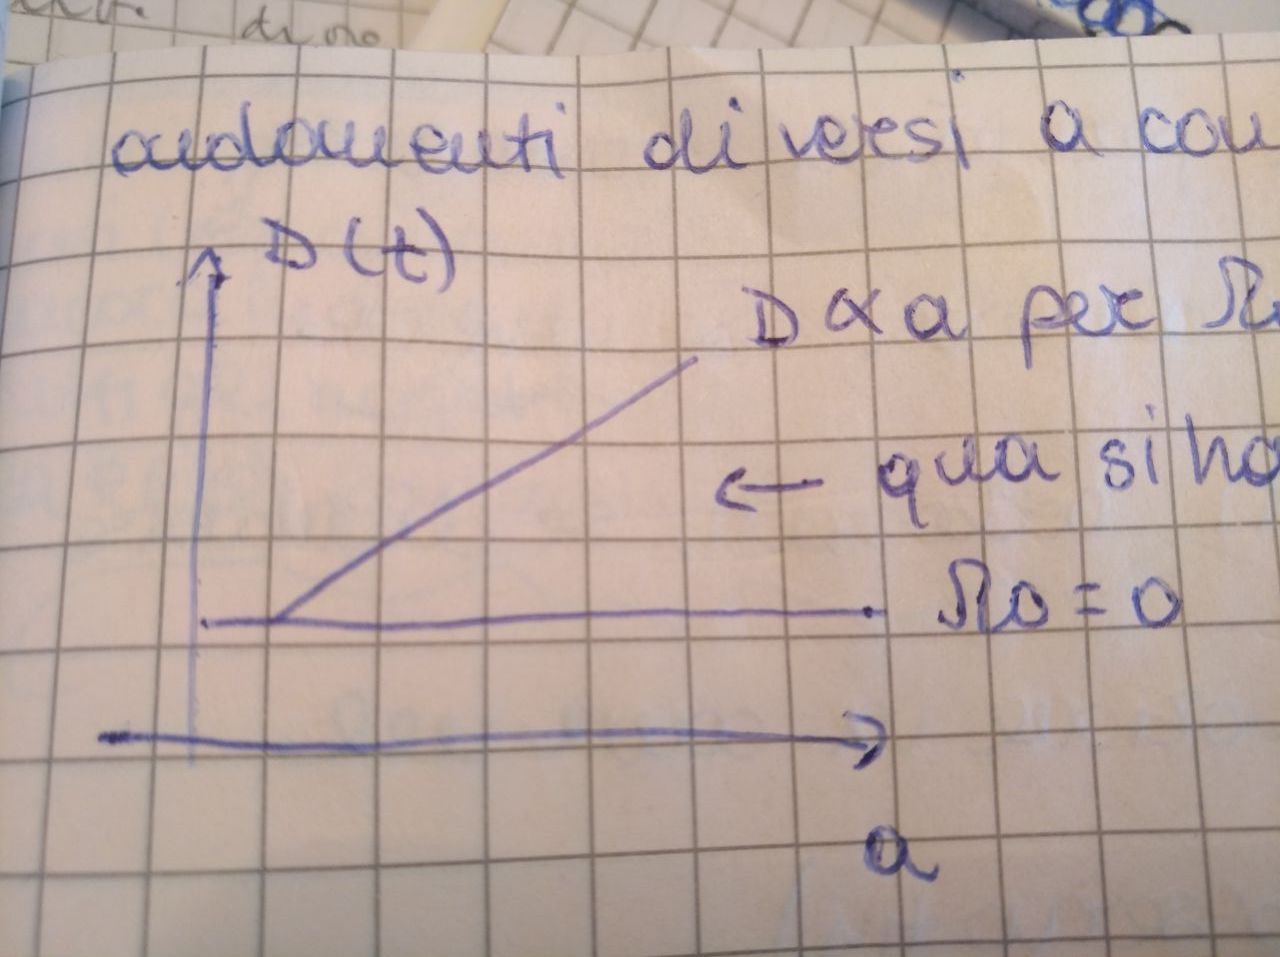
\includegraphics[width=8cm]{images/evD.jpeg}
\caption{Evoluzione del fattore di scala.}
\end{minipage}
\label{fig:massfunc}
\end{figure}
Il modello Bottom-Up produce un $M^{\star}$ crescente nel tempo secondo la definizione $M^{\star}(t)=\frac{\delta_c}{AD(t)}^{-\frac{n+3}{6}}$; dipende da  $D(t)$ che a sua volta dipende dal parametro $\Omega_0$. Si pu\'{o} misurare la densit\'{a} dell'universo con la funzione di massa delle strutture cosmiche poich\'{e} posso stimare la funzione di massa oggi e ad un epoca precedente; la misura cambia di poco dunque l'universo ha bassa densit\'{a} $\Omega_0=0.3$ \footnote{Infatti nel caso di universo vuoto $\Omega_0=0\Rightarrow D(t)=cost \Rightarrow M^{\star} =cost$.}. Attenzione perch\'{e} $M^{\star}$ dipende anche dalla \textbf{normalizzazione dello spettro di potenza}, e quindi posso avere $A$ grandi e $D(t)$ piccoli, si dice che si ha \textbf{degenerazione} tra i due fattori. La normalizzazione $A$ viene anche indicata nel seguente modo $\sigma^2_R(M)=\int_0^{\infty}P(k) k^2W^2(k,R)dk$ in cui una volta fissata la scala di massa $M$ o quella di lunghezza $R$ (che sono analoghe), $P(k)=Af(k)$ definisce la normalizzazione. Convenzionalmente si sceglie la lunghezza caratteristica $R=8\frac{Mpc}{h}$ per gli ammassi di galassie che fissa la normalizzazione a $A \equiv \sigma_{8}\simeq
1.7$. Tramite la funzione di massa possiamo misurare $\sigma_8$ che \'{e} degenere rispetto al fattore di crescita e quindi $\Omega_0$.
\begin{figure}[htp]
\centering
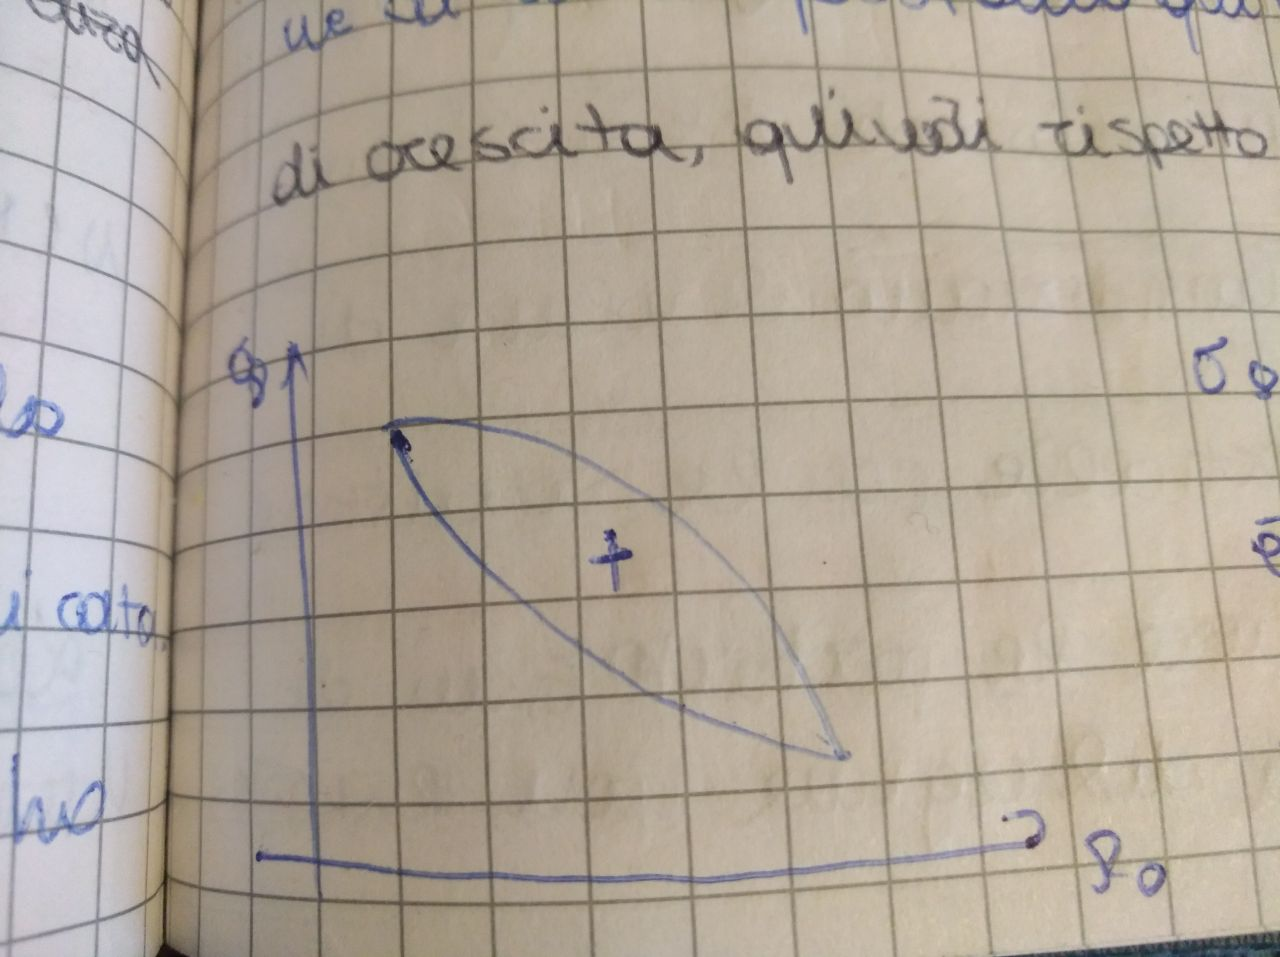
\includegraphics[width=7cm, height=7cm]{images/degSD.jpeg}
\caption{Degenerazione tra parametri $\sigma_8$ e $D$.}
\label{fig:degSD}
\end{figure}
Questi coefficinti sono anticorrelati:
\begin{itemize}
\item Grandi fluttuazioni $\sigma_8 \uparrow$ e bassa quantit\'{a} di materia$\Omega_0 \downarrow$
\item Molta materia $\Omega_0 \uparrow$ e basse fluttuazioni $\sigma_8 \downarrow$
\end{itemize}
Quando misuriamo la funzione di massa ne misuro la coppia. Quindi possiamo prendere indicativamente il valore medio per fissare questi parametri.\\
Devo ancora fissare la sovradensit\'{a} critica che fissiamo al valore dell'epoca della virializzazione $\delta_c=\delta_{vir}=1.68$, sto usando parametri estrapolati dalla teoria lineare in regime non lineare. Ora abbiamo tutti i parametri necessari per calcolare la funzione di massa. La confrontiamo con l'andamento calcolato da una simulazione ad N corpi con le condizioni iniziali definite nei paragrafi prima. Abbiamo un buon accordo tra i valori simulati e quelli misurati, ma possiamo ottenere dei miglioramenti. A livello \textit{teorico } $\delta_c$ non \'{e} esattamente quello previsto, \'{e} sottostimati di alcuni ordini di grandezza; anche lo sdoppiamento delle variabili anticorrelate pu\'{o} essere pi\'{u} accurato, possiamo ottenere un miglioramento inferiore al $10\%$. Dal punto di vista \textit{osservativo} dobbiamo determinare la funzione di massa quindi dobbiamo conoscere la massa degli ammassi di galassie, quindi per prima cosa dobbiamo avere dei cataloghi di ammassi ottenuti dallo studio della distribuzione delle galassie (correggo il Malmquist Bias se misuro da terra nella banda X) e secondariamente stimarne la massa attraverso metodi di \textbf{lente gravitazionale}. Con i vari metodi si trova pi\'{u} o meno lo stesso valore di $\sigma_8$ e $\Omega_0$. La funzione di massa \'{e} simile a quella di Luminosit\'{a} in quanto i parametri sono correlati $L\propto M^{\gamma}$.\\
Lo spettro di potenza deve essere collegato alle anisotropie del CMB, in quanto anisotropie del bagno di fotoni al disaccoppiamento radiazione materia.
\subsubsection{Anisotropie del CMB}
Le anisotropie del CMB non sono legate alla materia oscura poich\'{e} non ci sarebbe stato tempo di creare le strutture che abbiamo oggi. Invece abbiamo un legame con le perturbazioni di densit\'{a} della materia ordinaria. Le anisotropie si studiano attraverso il campo di temperatura $T(\theta, \phi)$, poich\'{e} possiamo associare ad ogni regione del cielo un corpo nero la cui emissione \'{e} una curva Planckiana. Analogamente alle perturbazioni di densit\'{a}, anche qui andiamo a definire la perturbazione del campo $T$ rispetto a $T_0$ come $\frac{\Delta T}{T_0}(\theta ,\phi)=\frac{T(\theta,\phi)-T_0}{T_0}$. Proseguendo sviluppiamo in armoniche sferiche.
\begin{equation}
\frac{\Delta T}{T_0}(\theta ,\phi)=\Sigma_{l=0}^{+\infty}\Sigma_{m=-l}^{+l}a_{l,m}Y_l^m(\theta,\phi)
\end{equation}
Poich\'{e} queste dipendono da Polinomi di Legendre allora soddisfano una relazione di ortogonalit\'{a}:
\begin{equation}
\int  Y_l^m(\theta,\phi)Y_{l'}^{\star m'}(\theta,\phi)d\Omega=\delta_{ll'}\delta_{mm'}
\end{equation}
Per misurare le perturbazioni di temperatura ($\frac{\Delta T}{T}$) sulla sfera celeste conviene andare nello spazio (satellite COBE) quindi ri ricavano i coefficienti dello sviluppo e lo spettro di potenza delle anisotropie:
\begin{equation}
\begin{cases}
a_{lm}=\int d\Omega \frac{\Delta T}{T}Y_l^{\star m}(\theta,\phi)
\\
C_l =\frac{1}{2l+1} \Sigma_{m=-l}^{+l} a_{lm} a_{lm}^{\star}=\langle \mid a_{lm}\mid^2\rangle_m
\end{cases}
\end{equation}
Essendo le anisotropie della gaussiane la descrizione completa su di esse \'{e} contenuto in $C_l$, che \'{e} l'analogo di $P(k)$. Gli "l" sono come i "k":
\begin{itemize}
\item grandi "l" $\Rightarrow$ piccola scala
\item piccoli "l" $\Rightarrow$ grande scala
\end{itemize}
Introduciamo la funzione di \textbf{autocorrelazione} a due punti della temperatura in coordinate angolari:
\begin{equation}
C(\theta)=\langle\frac{\Delta T}{T}(n_1) \frac{\Delta T}{T}(n_2) \rangle_{\Omega}  
\end{equation}
Ho la media sulla sfera celeste di due fluttuazioni in direzioni diverse tali che $n_1\cdot n_2=\cos{\theta}$. Sfruttando l'ortogonalit\'{a} delle armoniche sferiche si trova che la funzione di autocorrelazione \'{e} collegata allo spettro di potenza, esattamente come nelle perturb. di d.:
\begin{equation}
C(\theta)=\frac{1}{4\pi} \Sigma_l(2l+1)C_l\underbrace{ P_l(\cos{\theta})}_{p. Legendre}
\end{equation}
All'epoca del disaccoppiamento i $\gamma$ vengono diffusi dagli elettroni liberi, allora maggiore \'{e} la quantit\'{a} di elettroni maggiore sar\'{a} la quantit\'{a} di $\gamma$ diffusi. Qui si vede il collegamento tra le fluttuazioni di densit\'{a} e temperatura:
\begin{equation}
\frac{\Delta T}{T} \propto \frac{\delta\rho_b}{\rho_b} \propto \frac{\delta \phi}{\phi}
\end{equation}
Una grande concentrazione di materia significa una profonda buca di potenziale nella quale i fotoni diffonderanno molto. Per effetto di \textbf{redshift gravitazionale} i fotoni che escono dalla buca perdono energia e ci appaiono pi\'{u} rossi mentre quelli che cadono ci appariranno pi\'{u} blu acquisendo energia. La relazione di proporzionalit\'{a} $\frac{\Delta T}{T} \propto \frac{\delta\phi}{\phi}$ indica appunto la correlazione tra $C_l \leftrightarrow P(k)$ della materia barionica. \textit{Che relazione c'\'{e} tra fluttuazioni della CMB e materia oscura?} Ce lo dice l'orizzonte cosmologico che \'{e} dell'ordine di un paio di gradi, tutto quello a scala maggiore \'{e} al di fuori di esso. Quindi tutte le perturbazioni di densit\'{a} in materia barionica su scale pi\'{u} grandi di qualche grado non sono ancora entrate nell'orizzonte cosmologico e dunque riflettono le perturbazioni dell'epoca inflattiva. Proprio su queste scale allora le perturbazioni di materia barionica devono coincidere con quelle di materia oscura poich\'{e} essendo fuori dall'orizzonte cosmologico a quell'epoca, non hanno avuto il tempo di evolvere e comunicare. Si dimostra che la relazione che lega $C_l$ e $P(k)$ sia
\begin{equation}
C_l=\frac{1}{2\pi} \biggl( \frac{H_0}{c}\biggr)^4 \int_0^{\infty }P(k) J_l^2\biggl( \frac{2ck}{H_0}\biggl)\frac{dk}{k^2}
\end{equation}
Misurare $C_l$ su larga scala, ovvero con $l<100$ seleziono scale pi\'{u} grandi di qualche grado($\theta\sim \frac{\pi}{l}$), significa misurare $P(k)$ su scale pi\'{u} piccole dell'orizzonte cosmologico all'epoca del disaccoppiamento di radiazione e materia ovvero $P_{infl}(k)$ \footnote{La temperatura $T$ ha fatto cambiare lo spettro di H-Z a quello ad es. di CDM secondo la relazione $P_{eq}=T^2(k)P(k)$, questo avviene in quanto abbiamo una scala di FS.}. Siamo in zone in cui il FS non \'{e} avvenuto. Inserendo $P(k)=Ak^n$ spettro di potenza in $C_l$ si ottiene
\begin{equation}
C_l \propto 2^nA\pi \frac{\Gamma(3-n)\Gamma(l+\frac{n-1}{2})}{\Gamma^2(\frac{4-n}{2})\Gamma(l+\frac{5-n}{2})}
\end{equation}Dalla quale possiamo ricavare a grandi scale ($l\sim 100$) $A$ ed $n$ abbiamo allora un altro \textit{metodo}. Per $n\sim 1$ spettro di Harrison Zel'dovich $C_l\propto 2A\frac{1}{l(l+1)}$, che per $l \uparrow$ \'{e} pressoch\'{e} piatto, stiamo quindi misurando lo spettro inflattivo \footnote{In realt\'{a} $n\sim 0.97$.}. Sapere dove comincia $C_l$ quindi mi da $A$ e quindi $\sigma_8$, che oggi viene  misurato dall'esperimento Planck (misura lo spettro di potenza).  Si trova essere in accordo con quello misurato dalla funzione di massa degli ammassi di galassie. Questo non \'{e} sempre stato vero infatti il $\sigma_8$ misurato dagli ammassi era pi\'{u} piccolo di quello misurato dal CMB con COBE. Si ha quindi una possibile \textbf{misura diretta} del modello inflattivo, nel caso questo non dovesse corrispondere alla realt\'{a} abbiamo due possibili strade:
\begin{itemize}
\item trovare un modo per creare delle perturbazioni di densi\'{a} gaussiane con questo spettro di potenza
\item reinterpretare l'andamento delle anisotropie del CMB su queste scale.
\end{itemize}
Nel modello che abbiamo trovato l'andamento di $C_l$ coincide coincide con quello che ci aspettavamo, anzi permette di misurare i parametri. Se cambiasse il modello bisogna giustificare l'andamento di $C_l $ a grandi scale.
\subsubsection{Effetto Sachs-Wolfe}
Su larga scala, le anisotropie del CMB sono correlate alle fluttuazioni di densità dell'effetto Sachs-Wolfe (1967). Gli effetti gravitazionali delle perturbazioni della densità sul potenziale generano fluttuazioni di temperatura $\frac{\Delta T}{T}\propto\frac{\Delta \phi}{\phi}$ . Dalla RG l'energia necessaria per emergere da una buca di potenziale in uno spazio-tempo in espansione \'{e} dovuta a due fattori:
\begin{itemize}
\item campo gravitazionale 
\item espansione dell'universo
\end{itemize}

\begin{equation}
\frac{\Delta T}{T}\propto\frac{\delta \phi}{c^2}-\frac{2}{3}\frac{\delta t}{t}
\end{equation}
Il primo termine \'{e} dovuto al redshift gravitazionale (in uno spazio statico non in espansione), mentre il secondo \'{e} il termine ri ritardo relativistico dovuto al fatto che gli orologi in prossimit\'{a} della buca scorrono pi\'{u} lentamente (vediamo la regione pi\'{u} giovane, quindi pi\'{u} calda) \footnote{Siccome in EdS $T\propto a^{-1}\propto a^{-\frac{2}{3}}$, quindi abbiamo $\frac{\Delta T}{T}\propto\frac{2}{3}\frac{\delta \phi}{c^2}$.}. Considerando la perturbazione del potenziale nel caso classico in coordinate coomoventi e EdS vediamo che non dipende da $z$
\begin{equation}
\delta \phi\sim\frac{\delta\bar{\rho} R^3}{R}\sim\bar{\rho_0}(1+z)^3 \cdot \delta_0 (1+z)^{-1}\cdot R_0^2(1+z)^{-2} \sim\bar{\rho_0} \delta_0 R_0^2
\end{equation}
Siccome $\sigma_0=\langle \delta^2_0\rangle^{\frac{1}{2}}\sim \delta_0$ usando un filtro gaussiano $\sigma_0 \propto M_0^{-\frac{n+3}{6}}$ 
\begin{equation}
\delta_0\propto R_0^{\frac{1-n}{2}}
\end{equation}
Che si traduce in coordinate angolari $\theta\propto R_0$ \footnote{In quanto $\theta=\frac{R}{D_{A}}=\frac{R_0 a}{D_{A} a}$ nella quale $D\sim \frac{2c}{H_0 \Omega_0}=cost$ per $z\rightarrow \infty$.}
\begin{equation}
\delta \phi \propto \frac{\Delta T}{T}\propto \theta^{\frac{1-n}{2}}
\end{equation}
La fluttuazione in temperatura \'{e} indipendente dalla scala in EdS, e riproduce (per $n=1$) lo spettro di Harrison Zel'dovic, indipendente dalla scala (su larga scala). Oltre all'effetto Sachs-Wolfe che genera le anisotropie primarie del CMB, esiste anche un altro fenomeno che prende il nome di effetto \textbf{Rees-Sciama}. Questo genera delle anisotropie secondarie nel CMB in quanto i fotoni partiti dalla superficie di ultimo scatterning incontreranno nel loro cammino ottico perturbazione dello spazio tempo dovute alla presenza di materia. \'{E} fondamentale considerare l'evoluzione di queste perturbazioni di densit\'{a} perch\'{e} quando esce il fotone avr\'{a} una certa buca che sar\'{a} diversa alla sua uscita. Nel regime lineare la quantit\'{a} di energia che acquista un fotone in inflow \'{e} la stessa che perde in out. Nel regime non lineare questo non \'{e} pi\'{u} vero. Si potrebbe affermare che l'effetto di Rees-Sciama \'{e} l'analogo di Sachs-Wolfe ma nel caso non lineare. Si deve tenere conto di entrambe dal punto di vista statistico per avere informazioni sul modello inflattivo.
\subsection{Onde gravitazionali primordiali}
Nell'universo inflattivo si ha anche generazione di onde gravitazionali, con un loro spettro specifico. Ci\'{o} crea delle perturbazioni aggiuntive su piccola scala, poich\'{e} sono sorgenti di campo. Le perturbazioni di cui si \'{e} parlato fino ad ora sono perturbazioni di tipo \textbf{scalare} dovute alle fluttuazioni di densit\'{a} di materia. Quelle dovute alle onde gravitazionali sono variazioni della metrica $\frac{\delta g_{\mu \nu}}{g_{\mu \nu}}$, sono perturbazioni \textbf{tensoriali} che si aggiungono alle anisotropie scalari nel CMB. Si misurano nella fluttuazione della polarizzazione dei fotoni del CMB.
\subsection{Scale fisiche e angolari delle fluttuazioni}
Quando entriamo nell'orizzonte cosmologico $r_H$ \'{e} necessario stabilire quali processi fisici hanno determinato eventuali anisotropie del CMB \footnote{Le perturbazioni acustiche si generano per conpetizione tra due effetti, la pressione dei fotoni che tende a cancellare le anisotropie ed il Silk Damping tende a farele collassare formando delle strutture sovradense. Queste oscillazioni risultano nei picchi dello spettro della CMB.} quindi devo studiare le scale rilevanti che sono 2:
\begin{itemize}
\item (Scala $r_H$)
\item Scala di Jeans $\lambda_J$ caratterizza il collasso delle perturbazioni di densit\'{a}
\item Scala delle perturbazioni acustiche 
\end{itemize}
La scala dell'\textbf{orizzonte cosmologico} 
\begin{equation}
r_H=3ct\simeq \frac{2c}{H_0 \Omega_0^{\frac{1}{2}}}(1+z)^{-\frac{3}{2}} \approx 200 (\Omega_0 h^2)^{-\frac{1}{2}} Mpc
\end{equation}
siamo a $z\rightarrow 1000$ appena dopo l'epoca della ricombinazione (nello spettro di potenza abbiamo considerato $l=100$). Anche qui entrano in gioco i parametri cosmologici. Su scale pi\'{u} piccole abbiamo la diffusione di Thomson tra i fotoni e gli elettroni liberi che si stanno ricombinando con i protoni per formare idrogeno neutro.\\
La scala di \textbf{Jeans}
\begin{equation}
\lambda_J=\biggl(\frac{M_J}{\bar{\rho}_B}\biggr)^{\frac{1}{3}}\sim 50 \biggl(\Omega_b h^2\biggr)^{-\frac{1}{2}} Mpc
 \end{equation}
Se prendiamo come massa di Jeans $M_J\sim 10^{16} M_\odot$. In questo caso $\lambda_J$ dipender\'{a} dalla denist\'{a} barionica. La perturbazione si propaga con una velocit\'{a} $c_S$ di fluido relativistico, definiamo la scala dell'\textbf{orizzonte acustico} data dallo spazio percorso durante la vita dell'universo
\begin{equation}
\lambda_{SH}\simeq c_S t_{eta'} \leq \frac{c}{\sqrt{3}}t_{eta'}\sim 30 \biggl(\Omega_b h^2\biggr)^{-\frac{1}{2}} Mpc
\end{equation}
l'et\'{a} dell'universo la calcoliamo con i modelli di Friedmann e dipende da $\Omega_0$. Tipicamente $\lambda_{SH}<\lambda_J$ ma dipende da $\frac{\Omega_b}{\Omega_0}$. Su scale pi\'{u} piccole di $\lambda_J$ la perturbazione oscilla con frequenza $\omega^2= c_S^2k^2-4\pi G\bar{\rho}_B\approx c_S^2k^2$ in cui si trascura la componente di materia ordinaria che viene dall'equazione di Poisson. Questo ce lo dice l'instabilit\'{a} di Jeans in cui le perturbazioni con $\lambda<\lambda_J$ collassano per instabilit\'{a} gravitazionale, quindi aumenta la pressione favorendo una nuova espansione per poi ricollassare in seguito ad una diminuzione della pressione oscillando come onde acustiche.\\
Su scale al di sotto dell'orizzonte cosmologico  $r<r_H$ e al di sotto della scala di Jeans $\lambda<\lambda_J$ ci aspettiamo che le perturbazioni oscillino e che nel momento del disaccoppiamento radiazione materia, ipotizzando sia istantaneo, restino congelate in quella fase di oscillazione: se la perturbazione in quell'istante collassava allora rimarr\'{a} in quella fase, vale in viceversa. Si avranno una serie di perturbazioni su scale diverse.  Quindi per scale comprese tra $\lambda_{SH}<r<r_H$ le anisotropie che ci aspettiamo sono consistenti poich\'{e} la distribuzione di materia non \'{e} omogena al di sotto dell'orizzonte cosmologico. Ci saranno delle perturbazioni che si propagano in anisotropie della temperatura e saranno tipicamente correlate alle anisotropie sopra l'orizzonte cosmologico $\frac{\delta \rho}{\rho}\sim \frac{\Delta T}{T}$.
\begin{figure}[htp]
\centering
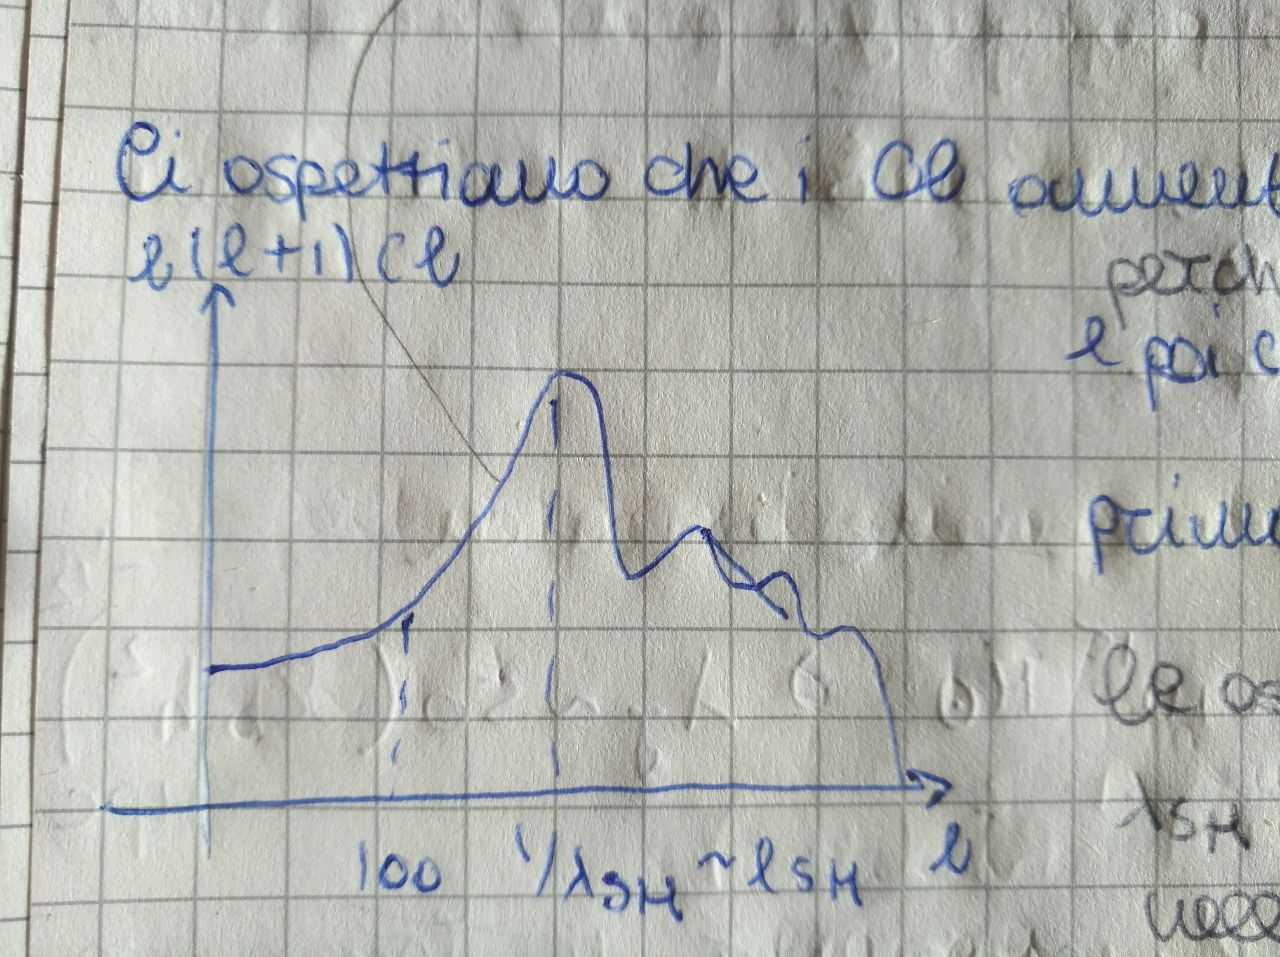
\includegraphics[width=7cm, height=7cm]{images/cmbfluc.jpeg}
\caption{Fluttuazioni della CMB.}
\label{fig:cmbfluc}
\end{figure}
Ci aspettiamo che all'aumentare di $l$, quindi al diminuire della scala, si raggiunga un picco e poi avremo ulteriori oscillazioni perch\'{e} le perturbazioni sotto l'orizzonte acustico oscillano. Il primo picco si ha in corrispondenza di $l_{SH}\sim \frac{1}{\lambda_{SH}}$ , in cui $\lambda_{SH}$ corrisponde ad una singola oscillazione tra l'entrata nell'orizzonte e la ricombinazione. In termini angolari la scala delle oscillazioni acustiche \'{e} $\theta=\frac{\lambda_{SH}^{prop}}{D_{A}}=\frac{\lambda_{SH}^{com}}{D}\approx 0.3 \Omega_0^{\frac{1}{2}}deg$, in cui la $D$ la ricavo dalla formula di Mattig, implicitamente sto considerando grandi $z$ e costante $\Lambda=0$. Siccome $\theta \sim \frac{\pi}{l}$, $l_{SH}$ corrisponde a questo $\theta$ quindi dipender\'{a} da $\Omega_0$: se il parametro cosmologico $\Omega_0 \uparrow$ \'{e} pi\'{u} grande allora il picco si sposta a scale pi\'{u} piccole $l\uparrow$, vale il viceversa. Facendo il conto accurato con $\Lambda \neq 0$  vediamo che  $\Omega_{k0}=\Omega_{\Lambda_0}-1$ quindi la\textit{posizione del picco dello spettro delle anisotropie del CMB \'{e} sensibile alla geometria dell'universo perch\'{e} dipende dalla distanza angolare}. Quindi possiamo usare la distanza angolare per misurare i parametri cosmologici , se si ha un oggetto di cui conosciamo le dimensioni proprie. Il nostro oggetto di riferimento sar\'{a} $\lambda_{SH}$ di cui conosciamo la distanza coomovente e propria alla ricombinazione. \textit{In sostanza il primo picco \'{e} una stima molto sensibile della ciurvatura spaziale dell'universo, che combinata con le osservazioni di Planck sul CMB si ottiene che la geometria spaziale dell'universo \'{e} euclidea quindi $\Omega_0+\Omega_{\Lambda0}=1$.}. Un altra relazione $\frac{\Omega_0}{2}-\Omega_{\Lambda0}=-\frac{1}{2}$, ci arriva dallo studio delle Supernovae, la cui sovrapposizione media a zero le anisotropie in temperatura in quanto alcune si contraggono e altre si espandono. I valori delle costanti che determiniamo sono concordi con le misure di massa e gli altri metodi visti in precedenza. Il disaccoppiamento ($z_{dis}=1070$) per\'{o} no \'{e} istantaneo, il lasso di tempo corrisponde ad una differenza di redshift $\Delta t_{dis}\rightarrow \Delta z \simeq 120$. Siccome $dz$ e $dr$ sono legati dalla relazione (per grandi $z$)
\begin{equation}
dr= \frac{cdz}{H_0 \Omega_0^{\frac{1}{2}}z^{\frac{3}{2}}}
\end{equation}
Stiamo implicitamente definendo un'altra scala, abbiamo che $\Delta z$ corrisponde a
\begin{equation}
\Delta r\simeq 10(\Omega_0 h^2)^{-\frac{1}{2}} Mpc
\end{equation}
la differenza spaziale che corrisponde alla periodo di disaccoppiamento radiazione materia, in sostanza coincide colla superficie di ultima diffusione, in realt\'{a} \'{e} un guscio spesso $\Delta r$ appunto, che osserviamo dalle anisotropie del CMB formate a $t\sim \Delta t_{dis}$:
\begin{itemize}
\item le perturbazioni con $r>\Delta r$, cio\'{e} pi\'{u} grandi della dello spessore di ultimo scattering, rimangono congelate nelle loro fase di contrazione o espansione.
\item mentre quelle con $r<\Delta r$ le perturbazioni non si traducono in anisotropie della $T$.
\end{itemize}
Quindi lo spettro di potenza, corrispondente alle anisotropie, si \textbf{smorza} notevolmente fino ad andare a zero. Questo fenomeno si combina con lo smorzamento di Silk descritto dalla scala tipica che per valori di $M_D=10^{12} M_\odot$ vale
\begin{equation}
\lambda_D\sim \biggl( \frac{M_D}{\bar{\rho_B}}\biggr)^{\frac{1}{3}} \sim 5 (\Omega_b h^2)^{\frac{1}{2}} Mpc.
\end{equation}
\textit{Questa scala, corrispondente al secondo picco, dipende da $\Omega_b$. Al di sotto di questa lo spettro delle anisotropie si annulla per la combinazione dell'effetto qui descritto in combinazione con lo smorzamento Silk (siamo a $l\sim 2500-3000$).}\\
Per ottenere una stima corretta dello spettro delle anisotropie del CMB\footnote{Sono flutuazioni in T che coincidono con le fluttuazioni di densit\'{a} in materia barionica.} si devono studiare le soluzioni dell'equazione di Boltzmann per un fluido collisionale in un universo in espansione, in cui si tiene conto del modello CDM
\begin{equation}
\ddot{\delta_B}+2 \frac{\dot{a}}{a}\dot{\delta}_B  =4 \pi G \rho_D \delta_D-\delta_B k^2 c_S^2.
\end{equation}
Le perturbazioni di densit\'{a} della DM, disaccoppiate dal resto,  hanno iniziato a collassare in epoca dell'equivalenza ora crescono e influenzano gravitazionalmente quelle di materia ordinaria, in quanto questa cade nelle buche di potenziale generate dalla DM. Trascurando il termine di espansione $\dot{a}=0$, ho un oscillatore armonico forzato, in qui la forzante \'{e} data dal potenziale della DM. 
\begin{equation}
\ddot{\delta_B}+ \delta_B k^2 c_S^2=4 \pi G \rho_D \delta_D
\end{equation}
Consideriamo perturbazioni del campo di radiazione ($\rho_r \sim T^4$)  \textbf{adiabatiche}, l'entropia viene conservata $\delta S=\delta \biggl(\frac{T^3}{\rho_m}\biggr) \Rightarrow 3\frac{\delta T}{T}=\frac{\delta \rho_m}{\rho_m}$. Mettendoci in un istante di tempo precedente al disaccoppiamento $\frac{\delta \rho_m}{\rho_m}=\frac{\delta \rho_B}{\rho_B} \Rightarrow \frac{\delta T}{T}=\frac{1}{3}\delta_B=\Theta$. con Definiamo $\psi=\delta \phi $ espansione in serie di onde piane del potenziale derivato dall'eq. $\nabla^2 \phi=4 \pi G \bar{\rho}_D \delta_D$, arriviamo ad una relazione alle derivate totali:
\begin{equation}
\begin{cases}
\ddot{\Theta}+k^2 c_S^2 \Theta=-\frac{1}{3}k^2 \psi
\\
c_S=\frac{c}{\sqrt{3(1+R)}}, \quad R=\frac{3\rho_B}{4\rho_r}
\end{cases}
\end{equation}
Considerando un fluido \textbf{non relativistico} (il caso relativistico si ha con $R=-1$). La soluzione \'{e} la seguente:
\begin{equation}
\Theta(t)=\biggl[ \Theta_0+\frac{1+R}{c^2}\psi \biggr]\cos{\omega t}+\frac{\Theta_0}{\omega}\sin{\omega t}-\frac{1+R}{c^2} \psi
\end{equation}
Abbiamo definito la frequenza come $\omega=kc_S$. Si osservi che questa soluzione \'{e} oscillatoria, siamo infatti a $\lambda <\lambda_J$, tuttavia \'{e} parziale perch\'{e} non tiene conto del redshift gravitazionale
\begin{equation}
\frac{\Delta T}{T}=\Theta_{ric}+\frac{\psi}{c^2}.
\end{equation}
Andiamo a studiare il comportamento dei picchi ($t=t_{ric} $), in cui sono contenute le informazioni di carattere cosmologico, imponendo le condizioni
\begin{equation}
\begin{cases}
\omega t_{ric}=k\lambda_{SH}=n\pi, \quad n\in \mathbb{N}
\\
\Theta_0=0
\\
\psi=\delta \phi=cost
\end{cases}
\end{equation}
osserviamo che $\Theta_0=0$ indica che la perturbazione \'{e} adiabatica, segue
\begin{equation}
\frac{\Delta T}{T}= \frac{\psi}{3c^2}[1+3R] \cos{\omega t}-\frac{R}{c}\psi
\end{equation}
ed infine considerando i massimi
\begin{equation}
\begin{cases}
\frac{\Delta T}{T}= \frac{\psi}{3c^2}[1+6R] \frac{\psi}{3c^2}, \quad k\lambda_{SH}=\pi
\\
\frac{\Delta T}{T}=\frac{1}{3} \frac{\psi}{c^2}\quad k\lambda_{SH}=2\pi
\end{cases}
\end{equation}
la prima definisce la massima compressione (si ritrova l'effetto Sachs-Wolfe) e la seconda la massima espansione, in quanto si definisce $\psi<0$ per le buche di potenziale. Quindi $\frac{\Delta T}{T}$ \'{e} negativo nel caso della massima espansione e positivo nella massima compressione. Tutto torna in quanto i fotoni perdono pi\'{u} energia all'aumentare della profondit\'{a} della buca.\\
Le fluttuazioni dello spettro della CMB dipendono dal parametro di Hubble "$h$".
\begin{figure}[htp]
\centering
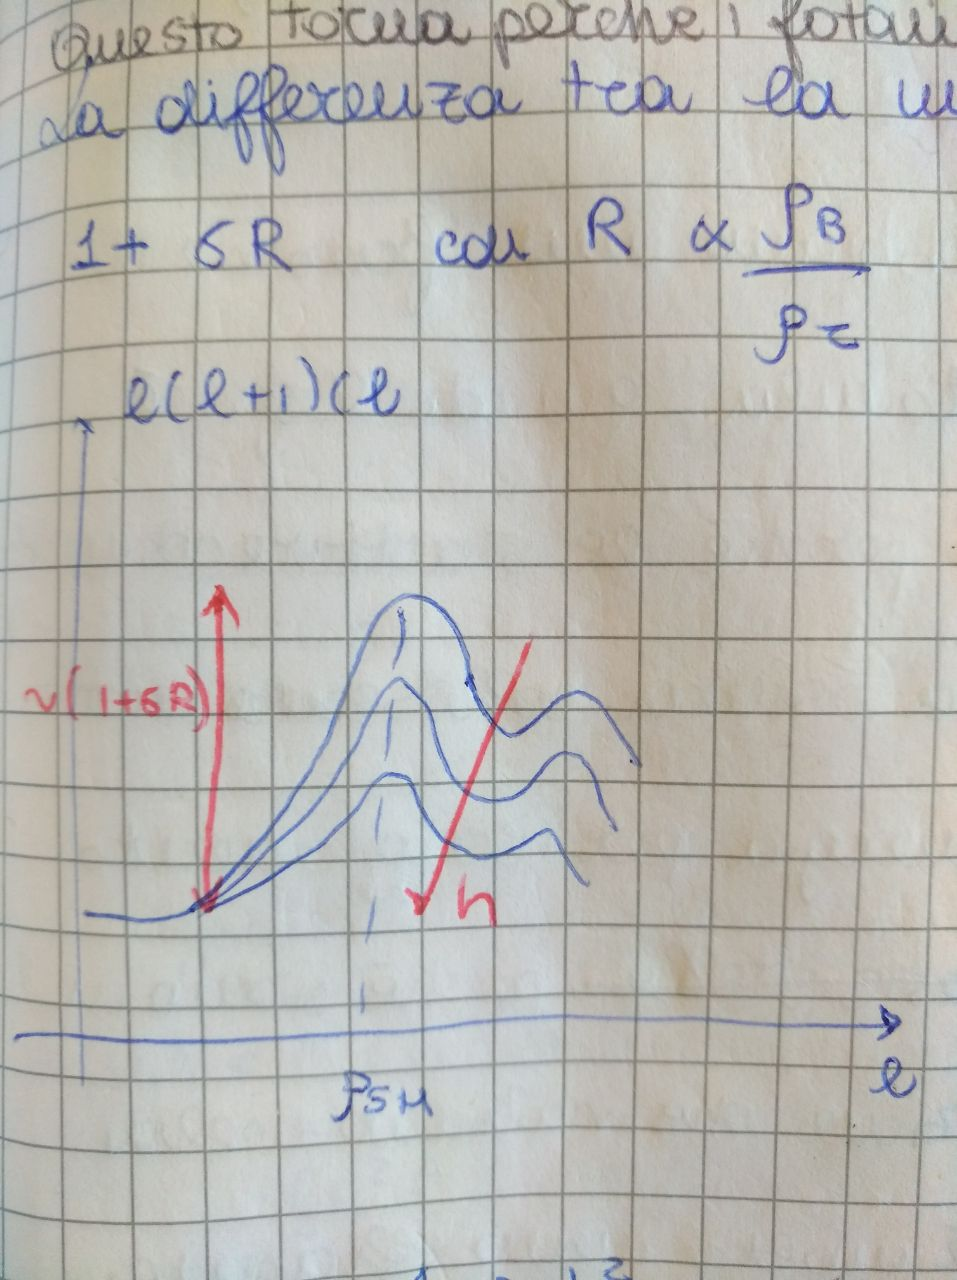
\includegraphics[width=7cm, height=7cm]{images/flucH.jpeg}
\caption{Fluttuazioni della CMB in funzione di h.}
\label{fig:flucH}
\end{figure}
\'{E} evidente che all'aumentare del parametro si allarga la finestra temporale tra $z_{eq}$ e $z_{ric}$, in quanto $z_{eq}\simeq 2.6 \cdot 10^{4} \Omega_0 h^2$ aumenta portando indietro l'epoca della ricombinazione. Ne consegue un abbassamento dello spettro. Si esprime la differenza tra la massima espansione e compressione attraverso il parametro $1+\sigma R$, con $R\propto \frac{\rho_B}{\rho_r}$. Quindi all'epoca della ricombinazione pi\'{u} aumento "$h$" e pi\'{u} $\rho_B$ si abbassa.
\begin{figure}[htp]
\centering
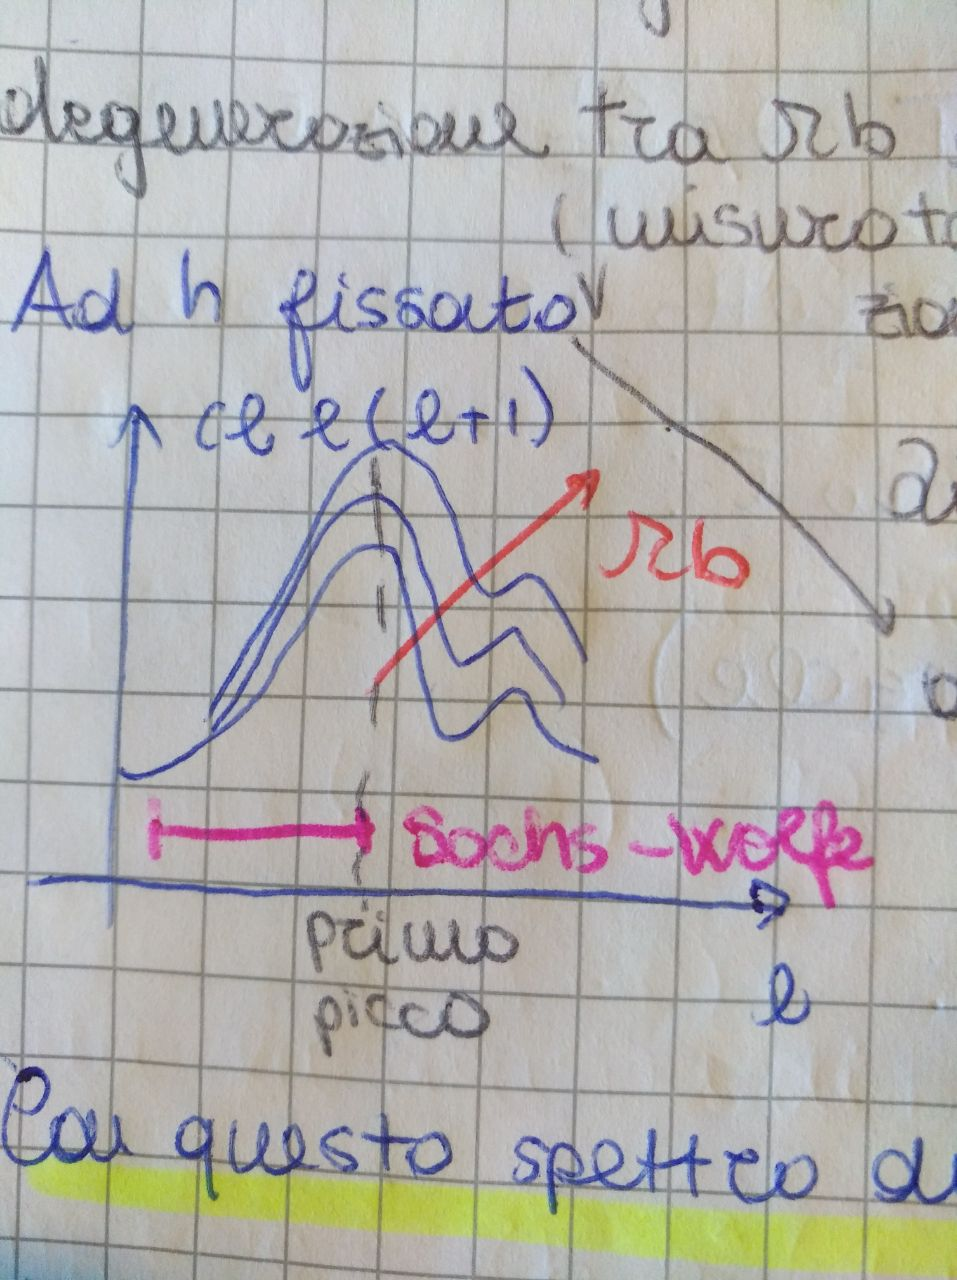
\includegraphics[width=7cm, height=7cm]{images/flucB.jpeg}
\caption{Fluttuazioni della CMB in funzione di $\Omega_B$.}
\label{fig:flucB}
\end{figure}
Cosa contraria invece per il parametro $\Omega_B$. Infatti i due parametri sono in anticorrelazione, si parla di degenerazione tra i parametri cosmologici ($h$, $\Omega_B$ e $\Omega_0$), infatti varie combinazioni ci danno lo stesso spettro.\\
\textit{In sintesi lo spettro di anisotropie del CMB \'{e} correlato allo spettro di potensa delle perturbazioni di densit\'{a}, quindi ricco di informazioni sull'universo primordiale. Andiamo per punti:}
\begin{itemize}
\item \textit{il primo picco determina la curvatura spaziale dell'universo, confermando $\Omega_0\sim 0.3$}
\item \textit{il secondo determina la densit\'{a} barionica $\Omega_B\sim 0.7$}
\item \textit{il terzo contiene informazioni sulla densit\'{a} di materia oscura}
\item \textit{i punti di massima espansione corrispondono ai minimi dello spettro}
\item \textit{le anisotropie primarie si sommano alle secondarie figlie dell'epoca di ricombinazione, quindi dell'effetto SZ, RS}
\item \textit{il fatto che l'universo abbia perturbazioni di densit\'{a} iniziali di tipo ingflattivo gaussiane \'{e } in ottimo accordo con lo spettro del CMB, e anche dall'evoluzione dell'instabilit\'{a} gravitazionale.}
\end{itemize}
\subsection{Mezzo intergalattico post-ricombinazione}
\textbf{Prima della ricombiazione} ($t<t_{ric}$) l'universo era opaco a causa dello scattering Thomson, come avevamo visto. Evolvendo diventa sempre pi\'{u} otticamente sottile (trasparente) mano a mano avviene la ricombinazione, quindi i protoni e gli elettroni si legano formando HI. Questo periodo viene definito come \textbf{Dark Age} poich\'{e} tutta la radiazione era costituita dalla CMB che era impegnata nello scattering, quindi non esistevano fotoni ed energie diverse.\\
Alla \textbf{ricombiazione} ($t=t_{ric}$) tutto il gas era praticamente neutro, la frazione di ionizzazione lo dimostra $\frac{HII}{HI}=10^{-5}$, non \'{e} un rapporto statico poich\'{e} la materia in inflow nella buca costituita DM si raffredda radiativamente ionizzando materia. L'universo non \'{e} trasparente alle radiazioni con lunghezze d'onda inferiori alla lunghezza d'onda di ionizzazione dell'idrogeno ($\SI{912}{\angstrom}$), né alle forti transizioni dell'idrogeno neutro, di cui $Ly\alpha$ è di gran lunga il più forte. Il fenomeno di "cooling" della materia in questione non \'{e} \textbf{efficiente} in quanto avendo unicamente idrogeno ho pochi canali di raffreddamento, dunque il processo di frammentazione delle nubi protostellari porta alla formazione di stelle molto massicce POPIII. Essendo composte per la maggior parte di H, il loro spettro piccato nell'alto UV ionizza il mezzo intergalattico, infatti il $75\%$ dei fotoni che emette $\lambda_{Ly \alpha}=\SI{1216}{\angstrom}$ corrispondono alla transizione Lyman $\alpha$ dell'atomo di idrogeno ($n=1 \rightarrow n=2$). Siamo nel periodo della \textbf{reionizzazione} 
\subsubsection{Sistema di assorbimento della serie di Lyman}
Quando la luce UV proveniente da una sorgente di background, in genere un \textbf{Quasar} o una \textbf{giovane galassia} con alta formazione stellare, viaggia attraverso lo spazio intergalattico, viene continuamente redshiftata prima di essere misurata dai nostri rilevatori. Nel suo cammino incontra sistemi di HI raggrumati e fluttuanti nella struttura filamentosa 2D su larga scala che costituisce lo space web. Questo \'{e} quella che viene definita \textbf{foresta Ly$\alpha$}, ovvero nubi di idrogeno neutro con densit\'{a} numerica che possiamo calcolarci in una metrica di FW dalle seguenti relazioni:
\begin{equation}
I=I_0 \exp{-\tau}
\end{equation}
\begin{equation}
\begin{cases}
\tau(\nu_o)=\int \alpha(\nu_e) \underbrace{cdt}_{dl}=\int_0^z \alpha(\nu_e) \frac{c dz'}{H_0 E^{\frac{1}{2}}(z') (1+z')}
\\
\alpha(\nu_e)=\sigma(\nu_e) n_{HI}(z)
\\
\sigma(\nu_e)=\frac{e^2f}{4\epsilon_0 m_e c}g(\nu_e-\nu_{Ly\alpha})
\end{cases}
\end{equation}
che mettendo tutto insieme ci porta a scrivere la profondit\'{a} ottica correlata al fotone osservato:
\begin{equation}
\tau(\nu_o)=\frac{e^2f}{4\epsilon_0 m_e c} \frac{1}{H_0} \frac{n_{HI}(z)}{(1+z)(\Omega_0 z+1)^{\frac{1}{2}}\nu_{Ly\alpha}}
\end{equation}
Conoscendo $I$ ed $I_0$ si trova il limite superiore della profondit\'{a} ottica $\tau \leq 0.1$ ovvero $n_{HI}(z=3)\leq 10^{-11}\frac{atomi}{cm^3}$, se la confrontiamo con la densit\'{a} di barioni $n_{b}(z=3)= 10^{-4}\frac{atomi}{cm^3}$ otteniamo $\frac{\Omega_{HI}}{\Omega_B}\sim 10^{-5}-10^{-6}$ sempre a $z=3$. La struttura d'idrogeno assorbe proporzionalmente alla sua densit\'{a} i fotoni che la attraversano, quindi il fatto che non assorba il flusso di UV che arriva dal quasar significa che la densit\'{a} di HI neutro \'{e} molto bassa in termini di densit\'{a} barionica.\\
\begin{figure}[htp]
\centering
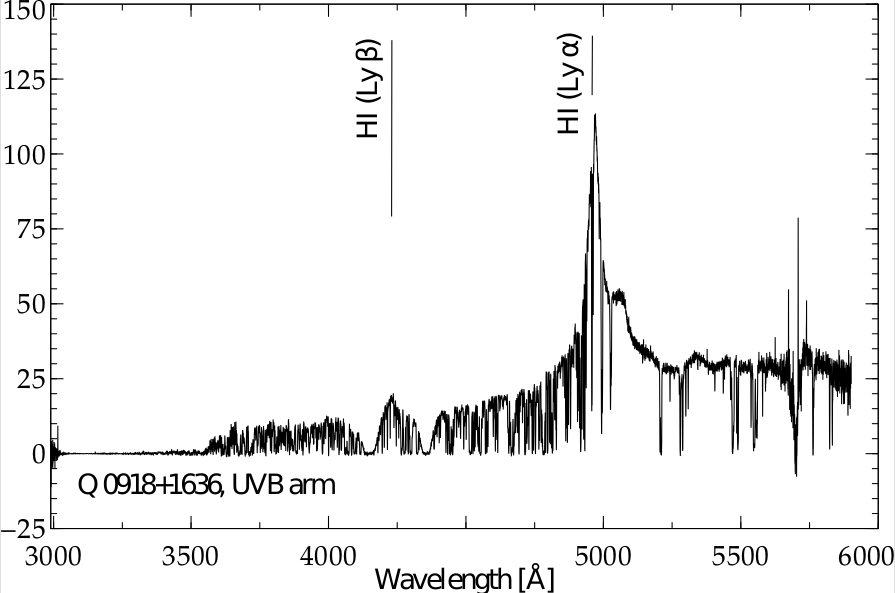
\includegraphics[width=7cm, height=7cm]{images/lyalpha.png}
\caption{Lo spettro del quasar viene frastagliato in seguito al passaggio dei suo fotoni attraverso il gas composto da idrogeno neutro. La profondit\'{a} della riga \'{e} correlata alla densit\'{a} barionica ad un certo redshift.}
\label{fig:lyalpha}
\end{figure}
Applicazioni cosmologiche:
\begin{itemize}
\item \textit{La mappatura della lunghezza d'onda e della distanza consente di mappare la densità di sistemi di diversa massa a diversi redshift lungo una certa linea di vista. La distribuzione di queste nuvole di HI segue quella di DM in quanto cadono dentro alle buche di potenziale della materia non barionica, quindi tracciano la distribuzione di massa dell'Universo, non solo la distribuzione della materia luminosa .}
\item \textit{Selezionando il limite superiore di densit\'{a} dell'idrogeno neutro abbiamo un metodo per cercare galassie in formazione.}
\end{itemize}
Siamo partiti all'epoca di ricombinazione $z\sim 1000$ in cui la frazione di ionizzazione era $\frac{HII}{HI}=10^{-5}$, nel frattempo avviene la \textbf{reionizzazione} fiono ad arrivare a $z\sim 3$ in cui arriviamo ad un limite in cui tutto l'idrogeno \'{e} ionizzato $\frac{HII}{HI}=10^{5}$. Nel lasso di tempo compreso tra $1000<z<3$ tutto l'idrogeno neutro \'{e} stato reionizzato da quasar e galassie giovani. \textit{Ci si domanda quanto il grosso della reionizzazione \'{e} avvenuto?}
\subsubsection{Depressione di Gunn-Peterson }
Per rispondere alla domanda posta in precedenza, bisogna andare ad osservare dei quasar che invece di avere nello spettro la foresta $Ly\alpha$ hanno una depressione dell'intensit\'{a} come mostrata nel grafico seguente.
\begin{figure}[htp]
\centering
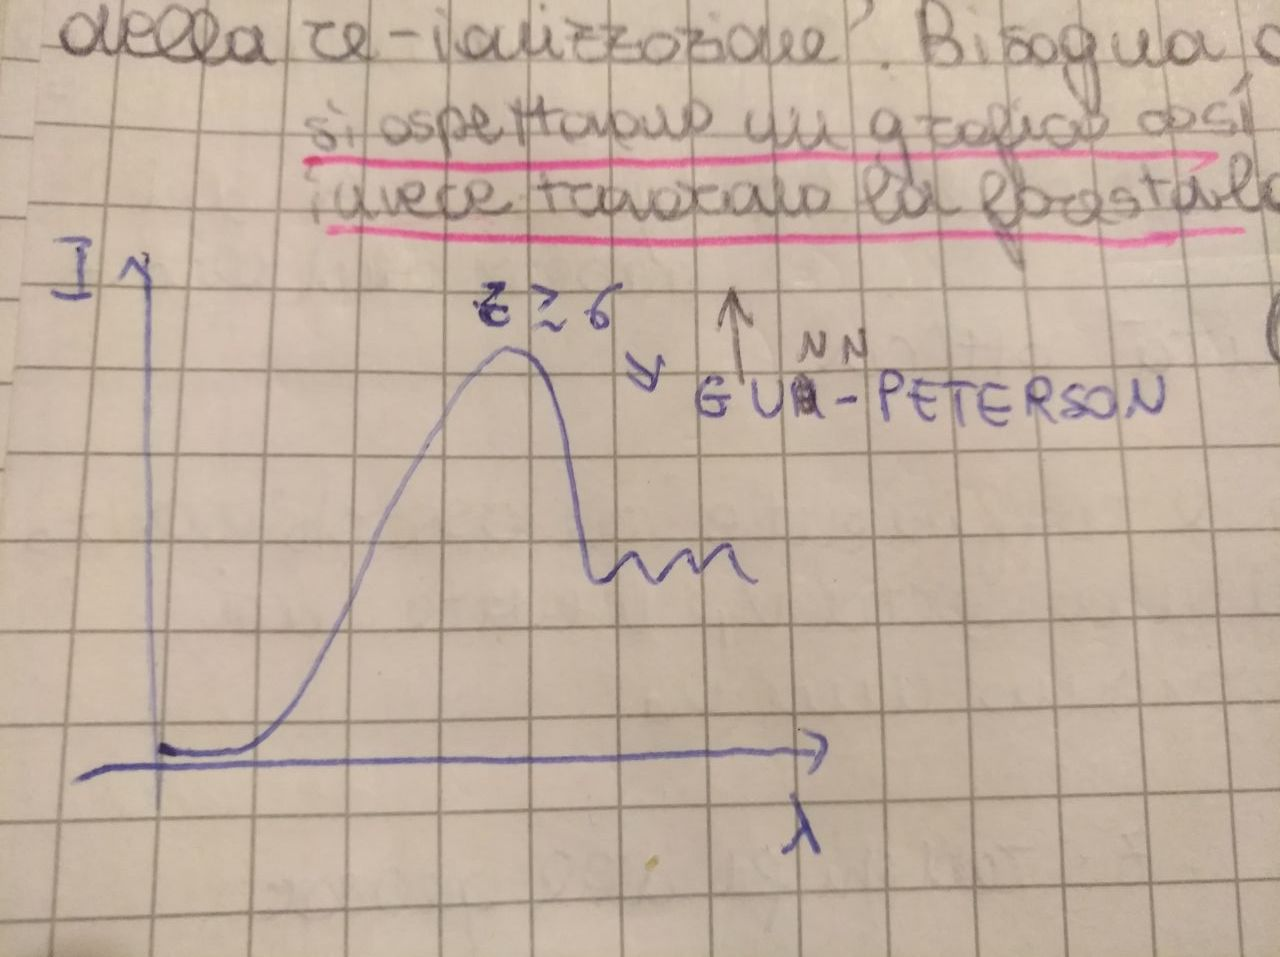
\includegraphics[width=6cm, height=6cm]{images/GunnPeterson.jpeg}
\caption{Lo spettro di Gunn Peterson non presenta le frastagliature che caratterizzavano la foresta Lyman $\alpha$.}
\label{fig:GunnPeterson}
\end{figure}
Nella figura\ref{fig:reioniz} la reionizzazione sembra completa già intorno a $z\sim8$, ma c'è ancora abbastanza idrogeno neutro che galleggia intorno per renderlo opaco a $Ly\alpha$ in quanto una piccola frazione $\frac{\Omega_{HI}}{\Omega_B}\sim 10^{-3}$ \'{e} sufficiente, quindi la $Ly\alpha$ definisce solo la vera fine del processo approssimativamente a $z\sim6$.\\
\begin{figure}[htp]
\centering
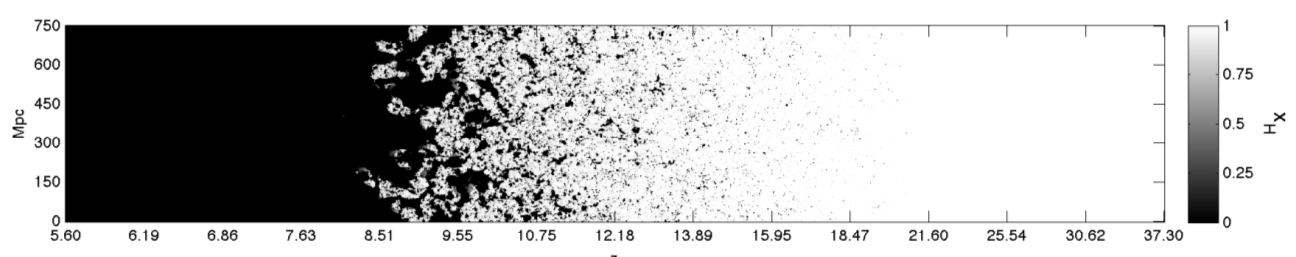
\includegraphics[width=17cm, height=4cm]{images/reioniz.png}
\caption{Mappa della reionizzazione in funzione del redshift.}
\label{fig:reioniz}
\end{figure}
\subsubsection{Ray Tacking Experiment}
Attorno agli anni '90 vennero fatte delle simulazioni ad N corpi  che simulavano l'universo (modello $\Lambda$CDM) nelle quali veniva simulata l'emissione di un quasar ad un estremo del dominio. Questo per avere le informazioni sull'universo a larga scala che derivo dall'assorbimento dello spettro da HI.
\subsubsection{Scale dinamiche e termiche}
Il gas ionizzato forma delle strutture cosmiche. Quindi regolare il processo \'{e} necessario prendere in considerazione le due scale che definiscono i processi che prendono parte: la scala dinamica che riguarda il collasso gravitazionale e la scala termica che riguarda la perdita di energia per irraggiamento.
\begin{equation}
\tau_{dyn}\sim (G\rho)^{-\frac{1}{2}}\propto n^{-\frac{1}{2}}
\end{equation}
Per introdurre l'altra forza che si oppone al collasso, ovvero quella di pressione, \'{e} necessario introdurre l'energia persa per collisionalmente per un gas ideale
\begin{equation}
\frac{dE}{dt}=-n^2 \Lambda(T)
\end{equation}
in cui $\Lambda$ \'{e} la funzione di raffreddamento dipendente dalla composizione chimica del plasma (per quella storia dei canali di raffreddamento) e alla velocit\'{a} con cui si muovono gli elettroni e gli ioni. Ad alte energie gli elettroni perdono energia per bremsstrahlung, radiazione da frenamento, mentre a basse energie perdono energia per ricombinazione.
\begin{figure}[htp]
\centering
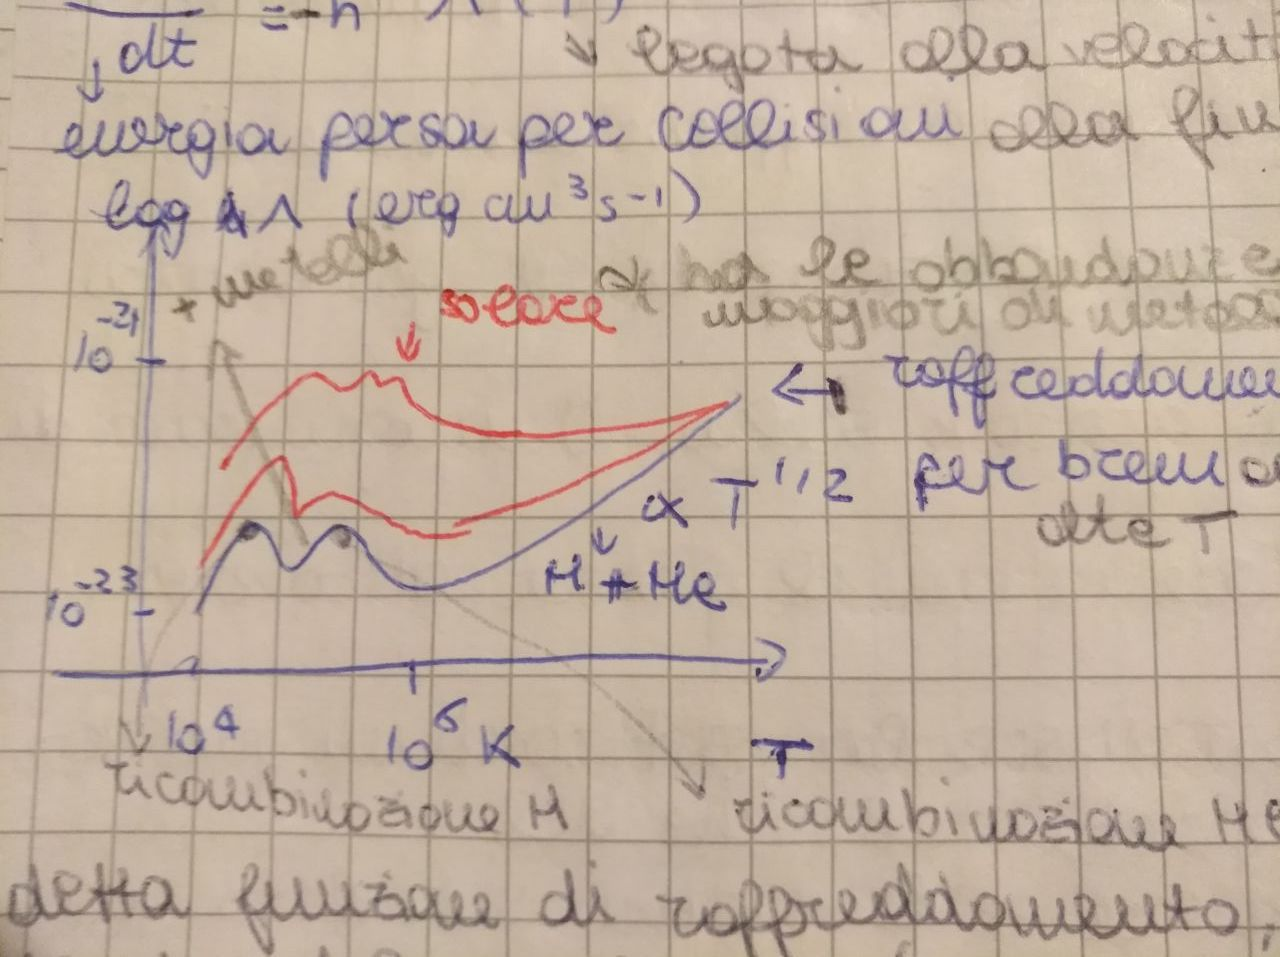
\includegraphics[width=7cm, height=7cm]{images/hratevst.jpeg}
\caption{\textbf{Curve di raffreddamento}: frazione di ionizzazione in funzione della temperatura.}
\label{fig:hratevst}
\end{figure}
\begin{equation}
\tau_{raff}=\frac{E_{in}}{\frac{dE}{dt}}=\frac{3k_B T}{n\Lambda(T)}
\end{equation}
Ora studiamo il collasso gravitazionale, il grafico \ref{fig:nvst} \'{e} sostanzialmente l'inverso delle curve di raffreddamento. 
\begin{figure}[htp]
\centering
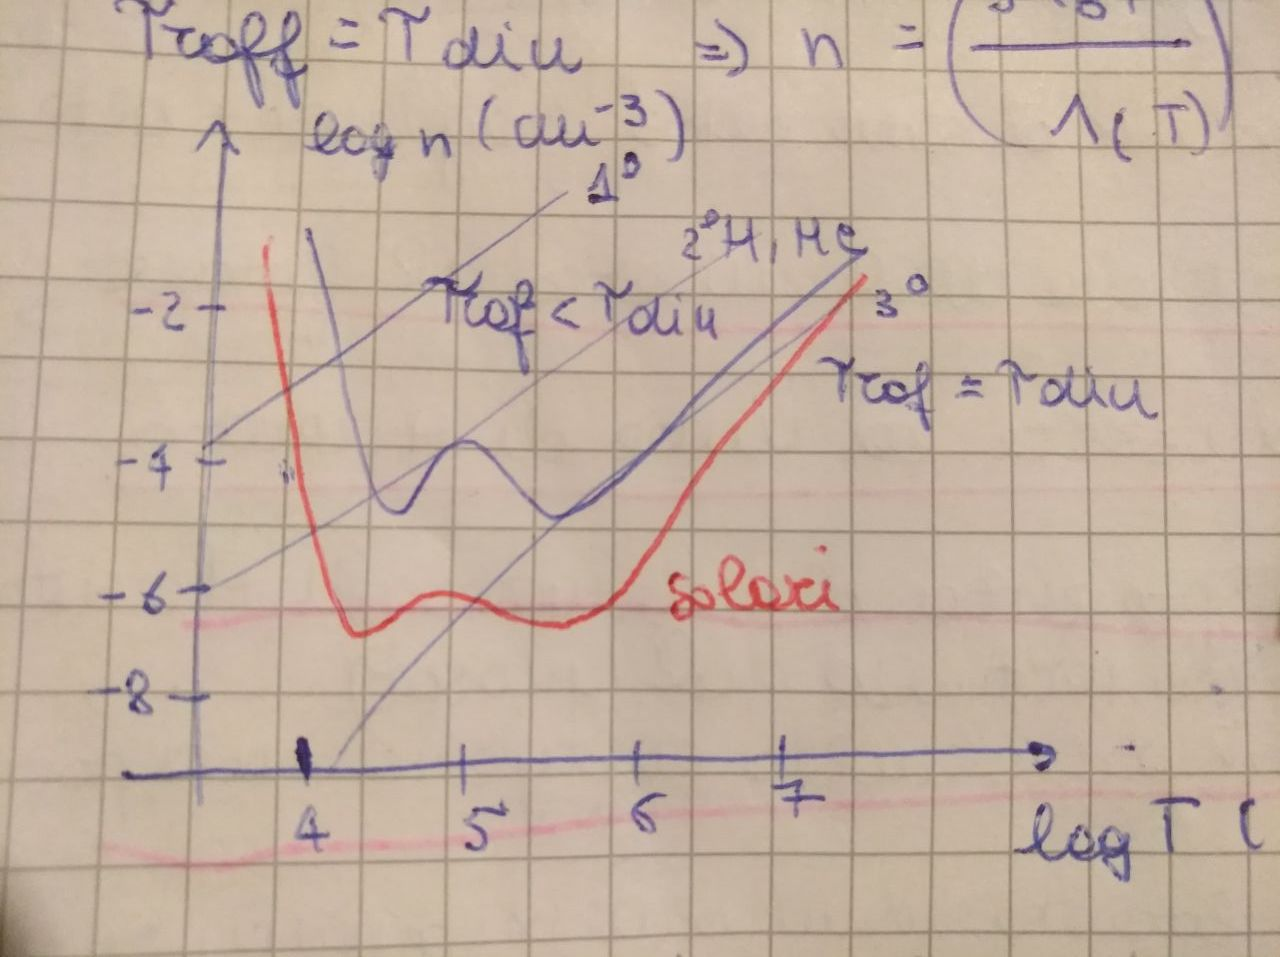
\includegraphics[width=7cm, height=7cm]{images/nvst.jpeg}
\caption{\textbf{Curve di collasso}: densit\'{a} in funzione della temperatura}
\label{fig:nvst}
\end{figure}
Per $\tau_{raff}<\tau_{dyn}$ quindi il gas si raffredda pi\'{u} rapidamente di quanto collassi: non c'\'{e} pi\'{u} la pressione a contrastare il collasso quindi la struttura collassa. Se a fissata temperatura considero la curva a densit\'{a} pi\'{u} basse la struttura sar\'{a} in equilibrio. Considerando in oggetto di massa costante si dimostra che $T\propto n^{\frac{1}{3}}$, quindi gli oggetti a massa costante nel grafico corrispondono a rette con la pendenza di $\frac{1}{3}$. Considerando tutti i coefficienti le varie curve corrispondono a masse:
\begin{equation}
\begin{cases}
M\sim 10^{10} M_\odot
\\
M\sim 10^{12} M_\odot
\\
M\sim 10^{14} M_\odot
\end{cases}
\end{equation}
Sulla terza retta stanno gli ammassi di galassie, il loro $\tau_{dyn} \sim \tau_{raff}$: la pressione del gas al loro interno impedisce il collasso gravitazionale. Infatti in queste strutture si ha per $(80-90)\%$ il gas a temperature $T\sim KeV$, il tasso di formazione stellare \'{e} molto basso in quanto il gas \'{e} rimasto caldo. Mentre sulla prima retta a $10 M_\odot$ , scala di massa galattica, la maggior parte del gas si \'{e} raffreddato formando stelle. Queste considerazioni ci danno un idea piuttosto qualitativa su che massa aspettarci nelle strutture barioniche, ma la questione \'{e} pi\'{u} complessa. Nel momento in cui il gas collassa per formare stelle pu\'{o} riscaldare a sua volta il messo intergalattico, esattamente come aveva ionizzato il gas. Si deve tenere conto del fatto che esistono problemi aperti nei \textbf{modelli di formazione stellare} a piccole scale, che possono essere originati da scala piccola o cosmologica. In questo tipo di formazione di strutture si riproduce in maniera qualitativamente corretta anche il fatto che regioni molto dense sono ricche di galassie ellittiche, viceversa quelle poco dense sono ricche di galassie a disco. Il quadro \'{e} corretto ma mancano una serie di dettagli, soprattutto nella formazione di galassie che coinvolga dalle scale atomiche a quelle cosmologiche. \\
L'epoca della ionizzazione sar\'{a} invece oggetto di survay radio, perch\'{e} vogliamo andare a vedere distribuzioni di  HI che emette nella riga a $\lambda > 21 cm$, da cui estrapoleremo informazioni sulla struttura a larga scala.
\end{document}